\chapter{Parametric model of a LEKID}\label{kid_model}

In the following, we develop a parametric model of a kinetic inductance detector (KID) which can be used to interpret or fit actual measurements produced by KID cameras or experiments. The model simulates both intrinsic circuit parameters and measured experimental values as a functions of base temperature \gls{Tbase} and absorbed optical power \gls{Pabs}. To be able to make accurate predictions, the model must incorporate the underlying device physics of KIDs. These physics are described within the framework of superconductivity.

The KID model contains several device properties which require initial values. These parameters, and the initial values which were used to produce the figures presented in the following sections, are listed in Table~\ref{table:kid sim}. The definition of each parameter can be found in the glossary section at the beginning of this document, or in the text below.

This chapter is organized as follows:

\begin{itemize}[nosep]
  \item Section~\ref{sec:supercond} provides a brief overview of relevant concepts from superconductivity.
  \item Section~\ref{sec:kinetic_inductance} introduces the kinetic inductance (KI).
  \item Section~\ref{sec:kid_params} describes the temperature and power dependence of key instrinsic and empirically determined values.
  \item Section~\ref{sec:responsivity} defines the KID responsivity to changes in \gls{Tc} (\gls{Rtemp}) and \gls{Pabs} (\gls{Ropt}).
  \item Section~\ref{sec:sensitivity} defines the instrumental sensitivity, and describes the instrumental noise budget for a KID instrument, detailing how each of the dominant noise sources contributes to the total noise-equivalent power (NEP).
\end{itemize}

\begin{table}[!htbp]
\centering
\begin{tabular}{@{}llll@{}}
\dtoprule{}
Parameter                         & 250~$\upmu$m         & 350~$\upmu$m         & 500~$\upmu$m         \\ \midrule
$w_{\mathrm{L}}$ ($\upmu$m)                  & 8                  & 10                 & 4                  \\
$l_{\mathrm{L}}$ ($\upmu$m)                  & 600                & 900                & 670                \\
$t_{\mathrm{L}}$ ($\upmu$m)                  & 18                 & 18                 & 20                 \\
\gls{N0} (ev$^{-1}$$\upmu$m$^{-3}$)     & 9.8 $\times$ 10$^{10}$ & 9.5 $\times$ 10$^{10}$ & 3 $\times$ 10$^{10}$ \\
\gls{Tc} (K)                         & 1.46               & 1.55               & 1.30               \\
$\tau_{\mathrm{rec},0}$ (s)                    & 3 $\times$ 10$^{-6}$ & 3 $\times$ 10$^{-6}$ & 3 $\times$ 10$^{-6}$ \\
$T_{\mathrm{LNA}}$ (K)            & 6                  & 6                  & 6                  \\
$Q_{\mathrm{loss}}$                        & 10$^{7}$           & 10$^{7}$           & 10$^{7}$           \\
\gls{Qc}                           & 4 $\times$ 10$^{4}$  & 4 $\times$ 10$^{4}$  & 4 $\times$ 10$^{4}$  \\
\gls{sig_n} ($\Omega$ cm)$^{-1}$ & 7000               & 7000               & 7000               \\
\gls{Tbase} (mK)          & 290                & 290                & 290                \\
\gls{Popt} (dBm)          & -90                & -90                & -90                \\
\gls{opt_eff}                     & 1                  & 1                  & 1                \\
\gls{det_eff}                     & 1                  & 1                  & 1                \\
\dbottomrule{}
\\
\end{tabular}
\centering
\caption[~Initial values of device parameters used in the KID model.]{Initial values of device parameters used in the KID model.}
\label{table:kid sim}
\end{table}

\section{Cooper Pairs and Quasiparticles}\label{sec:supercond}

A superconductor is a conductor whose DC resistance $R$ disappears when it is cooled below a material-specific temperature known as the critical temperature \gls{Tc}. The disappearance of $R$ is accompanied by the expulsion of magnetic field (B-field) lines from inside the material, which increases the magnetic flux at the surface. The latter phenomenon is known as the Meissner effect.

That $R$ goes to zero when a superconductor is cooled below \gls{Tc} implies (by Ohm's Law) that an infinite DC current can be generated by the application of a finite voltage. However, superconductors have non-zero impedance, because the reactance (capacitive and inductive) does not disappear along with $R$. The inductance of the superconductor prevents the instantaneous formation of an infinite current. Beyond a maximum current known as the critical current \gls{Ic}, the superconductor reverts to its normal state. Similarly, the superconductivity can be destroyed by applying a an external B-field whose strength exceeds the material's critical field $B_{c}$.

The underlying physics of superconductivity was first described by Bardeen-Cooper-Schrieffer (BCS) theory \citep{bardeen1957theory}. In BCS, when a superconductor is cooled below \gls{Tc} a supercurrent is created that consists of paired normal charge carriers (holes and electrons) called Cooper pairs (CPs). The remaining charge carriers which have not formed pairs are referred to as quasiparticles (QP). QP have the same spin and charge as normal electrons, but have an effective mass \gls{mstar} which differs from the rest mass of an electron \gls{m_e}.

CPs are modeled as quasi-bosons with mass of $2\gls{m_e}$ and charge of $2e$. The pairs arise from electron-phonon interactions in the crystal lattice of the conductor. Cooling the material decreases the thermal vibrations in the cation lattice. A single QP moving through the lattice attracts several cations, creating a local overdensity of positive charge, or a phonon, which propagates along with the QP. A second QP, having opposite spin to the first, becomes attracted to the phonon, forming the second member of the CP. The pairs have coherence lengths which are typically several orders of magnitude greater than the lattice spacing.

From an energy standpoint, the formation of supercurrent is the consequence of the creation of an energy band gap which forms above and below the material's Fermi energy:

\begin{equation}\label{eq:bandgap}
  E_{g}(T = 0) = \gls{Delta} = \frac{3.52}{2}k\gls{Tc}
\end{equation}

where $k$ is Boltzmann's constant, and \gls{Delta} is the value of the band gap at absolute-zero. The Fermi energy, $E_{F}$, is the difference in the energy between the highest and lowest states which are occupied by the fermions (electrons and holes) at $T = 0$~K \citep{kittel1998thermal}:

\begin{equation}\label{eq:Fermi_energy}
  E_{F} = \frac{\hbar^{2}}{2 \gls{mstar}}\left( \frac{3 \pi^{2} \gls{N0}}{\Sigma} \right)
\end{equation}

where $\Sigma$ is the volume of the conductor, and \gls{N0} is the single-spin density of states at the Fermi energy. During cooling, the rate of the decline in $R$ with $T$ is material dependent. For example, the decline is much faster in aluminum (Al) devices than in titanium nitride (TiN) devices \citep{mauskopf2018transition}. The band gap energy \gls{Delta} is equivalent to the CP binding energy, and is typically of $\mathcal{O}(10^{-3})$~eV. This band gap is around three orders of magnitude smaller than that of semiconductors, including CCDs, which illustrates the potential sensitivity advantages of using superconductors as detectors.

Any energy greater than $2\gls{Delta}$ which is absorbed by a superconductor will unbind, or break apart a CP into its constituent QP\@. This breaking apart of CPs can be measured to estimate the total power which is absorbed by a device. In the case of a KID, the splitting of CPs is measured by proxy, using the corresponding change in KI (see Section~\ref{sec:kinetic_inductance}). In Section~\ref{QP} we will derive an equation which contains the band gap energy's dependence on \gls{Tc} and \gls{Pabs}.

\subsection{Quasiparticle Generation and Recombination}\label{QP}

In a KID, QP are generated and recombine (CPs dissociate and reform) due to the absorption of thermally generated phonons in the material. These phonons may be produced by temperature fluctuations in \gls{Tbase}, or from power dissipated by the microwave carrier tone which is used to readout the device. QP are also generated by the absorption of photons with frequency $\nu \geq 2\gls{Delta}/h$. In the superconducting materials used to fabricate sub-mm/mm-wave KID devices, typical QP lifetimes (recombination times) \gls{tau_qp}, are $\mathcal{O}$(10)~$\upmu$s. An empirical expression for the QP lifetime which has been found to apply to several materials is \citep{zmuidzinas2012superconducting}:

\begin{equation}\label{eq:tau_qp}
  \gls{tau_qp} = \frac{\tau_{max}}{1 + \gls{nqp}(T)/n^{\star}}
\end{equation}

where $\gls{nqp}(T)$ is the number density of thermally generated QP, and $n^{\star}$ $\sim$ 100~$\upmu$s is the cross-over number density. The QP which are generated by thermal phonon absorption and by pair-breaking photons can be modeled as two distinct populations.

The total number density of QP is \citep{mauskopf2018transition}:

\begin{equation}\label{eq:nqp_tot}
  \begin{aligned}
  n_{qp,\mathrm{tot}} &= \gls{nqp}(T) + \gls{nqp}(P) \\
          &= 4\gls{N0} \int_{0}^{\infty} \frac{dE}{1 + e^{E/k\gls{Tc}}} \\
          &= 4N_{0}k\gls{Tc}\text{ln(2)}
  \end{aligned}
\end{equation}

To separate out the effects of varying \gls{Tbase} and \gls{Pabs}, the thermal and optical QP number densities must be written explicitly. In the low temperature limit ($T \ll \gls{Tc}$) the number density of thermal QP is

% QP number density
\begin{equation}\label{eq:Nqp_T}
  \begin{aligned}
  \gls{nqp}(T) &\simeq 2\gls{N0}\sqrt{2\pi k T \gls{Delta}}e^{-\gls{Delta}/kT} \\
               &= \frac{\gls{Nqp}(T)}{\Sigma}
  \end{aligned}
\end{equation}

\begin{comment}
\begin{equation}\label{eq:density of states}
   \gls{N0} = \frac{\Sigma}{3\pi^{2}} \left( \frac{2 E_{F} \gls{mstar}} { \hbar^{2} } \right)^{3/2}
\end{equation}
\end{comment}

where $\Sigma$ is the volume of the inductor, and $\gls{Nqp}(T)$ is the total number of thermally generated QP\@.  Figure~\ref{fig:Nqp_T} shows $\gls{Nqp}(T)$ for a range of base temperatures.

The number of QP produced per absorbed photon of frequency $\nu$ can be found by taking the ratio of the photon energy to the band gap energy:

% number of QP per photon
\begin{equation}\label{eq:qp_per_photon}
  \gls{Nqp}(\nu)_{\mathrm{,per}} = \frac{\gls{det_eff} h\nu}{\gls{Delta}}
\end{equation}

where \gls{det_eff} is the detector quantum efficiency (typically $\sim$80\%). The number of broken CPs per absorbed photon would be half of Equation~\ref{eq:qp_per_photon}. The corresponding number of optically generated QP is:

% number of optically generated QP
\begin{equation}\label{eq:Nqp_P}
  \begin{aligned}
  \gls{Nqp}(P) &= \frac{ \gls{det_eff}\gls{opt_eff} \gls{Nqp}(\nu)_{\mathrm{,per}} \gls{Pabs}\gls{tau_qp}}{h\nu} \\
              &= \frac{\gls{Nqp}(\nu)_{\mathrm{,per}}\gls{Popt}\gls{tau_qp}}{h\nu}
  \end{aligned}
\end{equation}

\begin{figure}[!htbp]
\centering
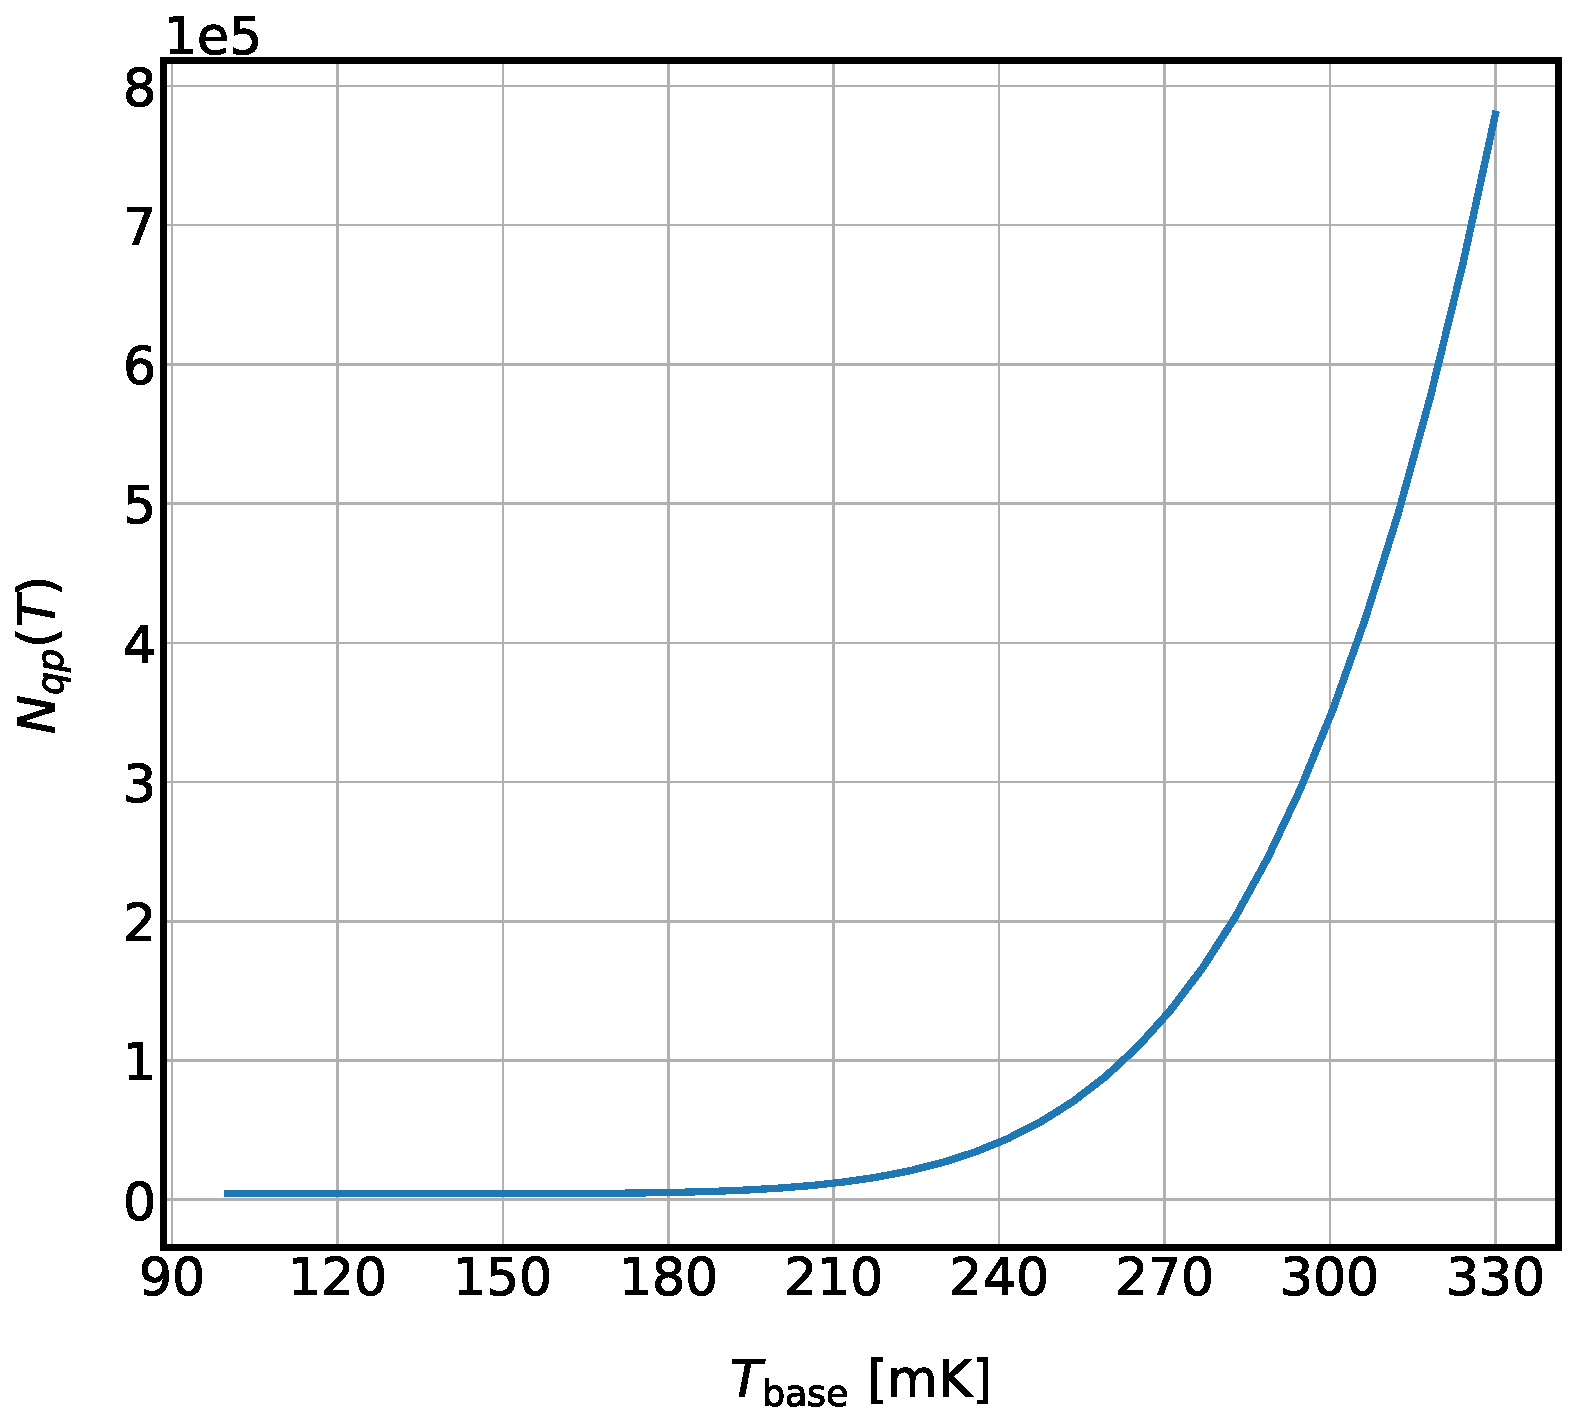
\includegraphics[width=\textwidth]{figures/kid_model/Nqp_T}
\caption[~\macrocapwrap{\gls{Nqp}} as a function of base temperature.]{The total number of thermally generated QP as a function of base temperature.}
\label{fig:Nqp_T}
\end{figure}

\begin{figure}[!htbp]
\centering
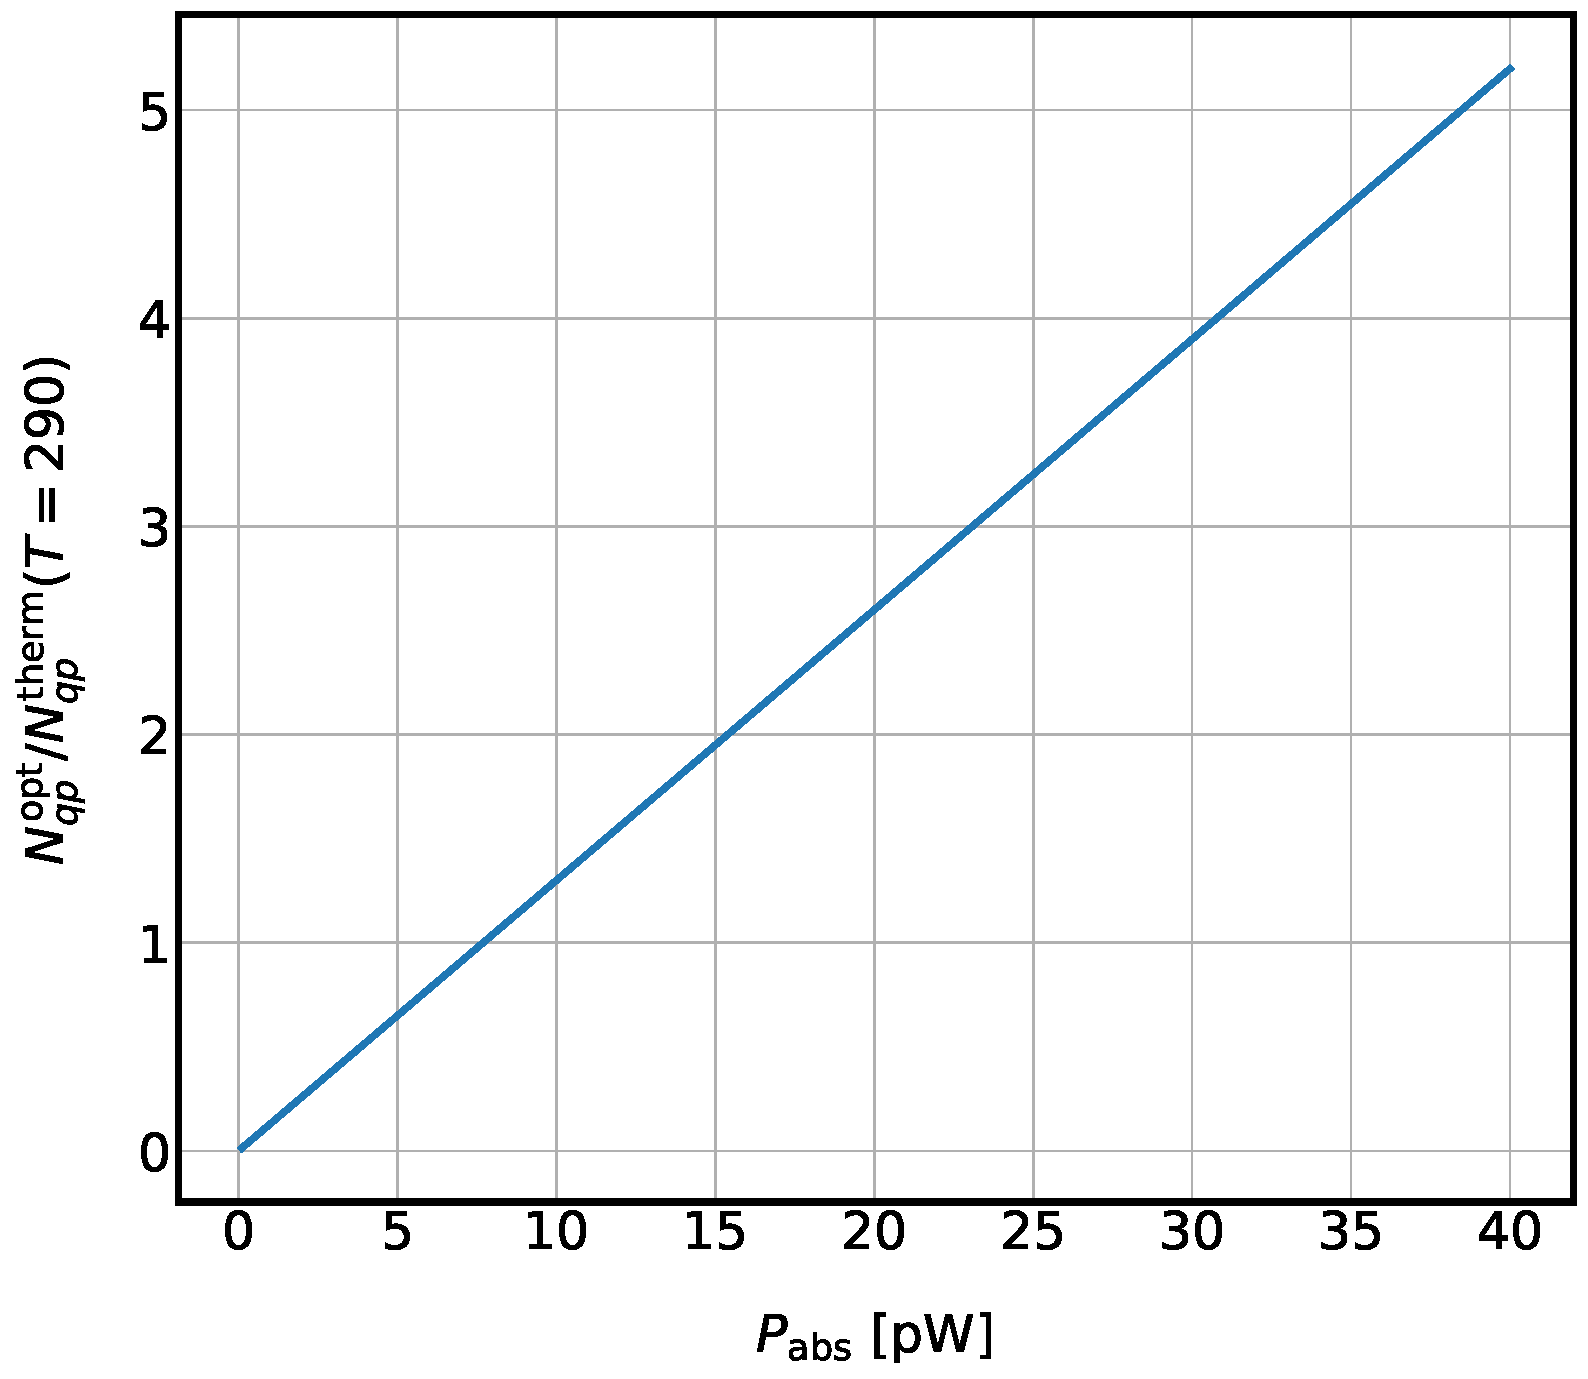
\includegraphics[width=\textwidth]{figures/kid_model/Nqp_ratio}
\caption[~The ratio of the number of optically generated to thermally generated QP as a function of absorbed optical power.]{The ratio of the number of optically generated QP to thermally generated QP, $N_{qp,\mathrm{opt}}/N_{qp,\mathrm{therm}}$, as a function of \gls{Pabs}. \gls{Tbase} is fixed at 290~mK.}
\label{fig:Nrat}
\end{figure}

The ratio $\gls{Nqp}(P)/\gls{Nqp}(T = 290)$ is shown in Figure~\ref{fig:Nrat} for a range of \gls{Pabs}, with $\gls{Tbase} = 290$~mK. Using Equations~\ref{eq:Nqp_T} and~\ref{eq:Nqp_P} to express the total number of QP $N_{qp,\mathrm{,tot}}$, the band gap energy can now be expressed as a function of both \gls{Tc} and \gls{Pabs}:

% Delta as function of Nqp_tot
\begin{equation}
 \Delta(T,P) = \frac{\gls{Delta}}{2}\left( 1 + \sqrt{1 - \frac{2\gls{Nqp}_{\mathrm{,tot}}} {\Sigma\gls{N0}\gls{Delta}}} \right)
\end{equation}

\subsection{The Two-Fluid Model}\label{two_fluid_model}

Several of the KID parameters discussed in the following sections depend on the conductivity $\sigma$ of the superconductor. Here we describe the two-fluid model of conductivity (\citet{glover1957conductivity,mattis1958theory}), which relates the Drude conductivity \gls{sig_d} in a normal conductor to the CPs and QP of a superconductor.

In a conductor, the equation of motion for a charge carrier is:

\begin{equation}
  \gls{mstar}\dot{v} = -eE - \frac{\gls{mstar}v}{\gls{tau_s}}
\end{equation}

where $\omega$ is the frequency of a time-varying electromotive force (EMF) being applied to the circuit, \gls{mstar} is the effective mass of the charge carrier, and $\boldsymbol{v}$ is their drift velocity ($\propto e^{j\omega\gls{tau_s}}$). The second term on the right-hand side of the equation is a damping term which accounts for charges scattering off of the lattice, with \gls{tau_s} being the characteristic time between collisions. Ohm's Law provides the relation between conductivity and current density: $J = \gls{sig_d} E$, with $J = n_{e}ev$.

Inserting these relations into the equation of motion, and solving for \gls{sig_d} yields the Drude conductivity:

\begin{equation}\label{eq:drude}
  \begin{aligned}
  \gls{sig_d}(\omega) &= \frac{n_{e}e^{2}\gls{tau_s}}{m_{e}}\frac{1}{1 + j\omega\tau} \\
                 &= \frac{\sigma_{n}}{1 + j\omega\gls{tau_s}} \\
                 &= \frac{\gls{sig_n}}{1 + \omega^{2}\gls{tau_s}^{2}} - j\frac{\gls{sig_n}\gls{tau_s}}{1 + \omega^{2}\gls{tau_s}^{2}} \\
                 &= \gls{sig1} - j\gls{sig2}
  \end{aligned}
\end{equation}

where \gls{sig_n} is the normal conductivity, $\gls{sig_n} = n_{e}e^{2}\gls{tau_s}/\gls{mstar}$. In a normal metal, \gls{tau_s} is small enough so that $\gls{sig_d} \approx \gls{sig_n}$ is negligible at frequencies $\omega$ below the optical range. For $kT \ll \gls{Delta}$ and $\hbar \omega \ll \gls{Delta}$, the real and imaginary conductivities can be written as \citep{gao2008physics}:

% sig1 thermal
\begin{equation}
  \gls{sig1}(\gls{nqp}, T)_{\mathrm{therm}} = \frac{4\gls{sig_n}\gls{Delta}}{\hbar \omega}e^{-\frac{\gls{Delta} - \upmu^{*}}{kT}}\sinh(\xi)\gls{K0}(\xi)
\end{equation}

% sig2 thermal
\begin{equation}
  \gls{sig2}(\gls{nqp}, T)_{\mathrm{therm}} = \frac{\gls{sig_n}\gls{Delta}}{\hbar \omega}\Bigg[ 1 - \sqrt{ \frac{ 2\pi kT }{ \gls{Delta} } } e^{-\frac{\gls{Delta}}{kT}}
   - 2e^{ \frac{\gls{Delta}}{kT}} e^{-\xi} \gls{I0} \Bigg]
\end{equation}

% sig 1 optical
\begin{equation}
  \gls{sig1}(\gls{nqp}, T)_{\mathrm{opt}} = \frac{2\gls{Delta}}{\hbar \omega} \frac{ \gls{nqp}} { 2\gls{N0}\sqrt{\pi kT\gls{Delta}}}\sinh(\xi)\gls{K0}(\xi)
\end{equation}

% sig2 optical
\begin{equation}
  \gls{sig2}(\gls{nqp}, T)_{\mathrm{opt}} = \frac{ \pi\gls{Delta} }{ \hbar\omega } \Bigg[ 1 - \frac{ \gls{nqp} }{ 2\gls{N0}\gls{Delta} } \left( 1 +
  \sqrt{ \frac{ 2 \gls{Delta} }{ \pi kT } } e^{-\xi} \gls{I0} \right) \Bigg]
\end{equation}

Figure~\ref{fig:sig_ratio_T} shows the ratio of \gls{sig1} to \gls{sig2} as a function of \gls{Tbase} ($\gls{Pabs} = 0$). The ratio asymptotically decays to zero for $T \gtrsim 250$~mK. The ratio of \gls{sig1} to \gls{sig2} as a function of \gls{Pabs} ($\gls{Tbase} = 290$~mK) is shown in Figure~\ref{fig:sig_ratio_P}. The ratio falls below one for $\gls{Pabs} \gtrsim 12$~pW.

\begin{figure}[!htbp]
\centering
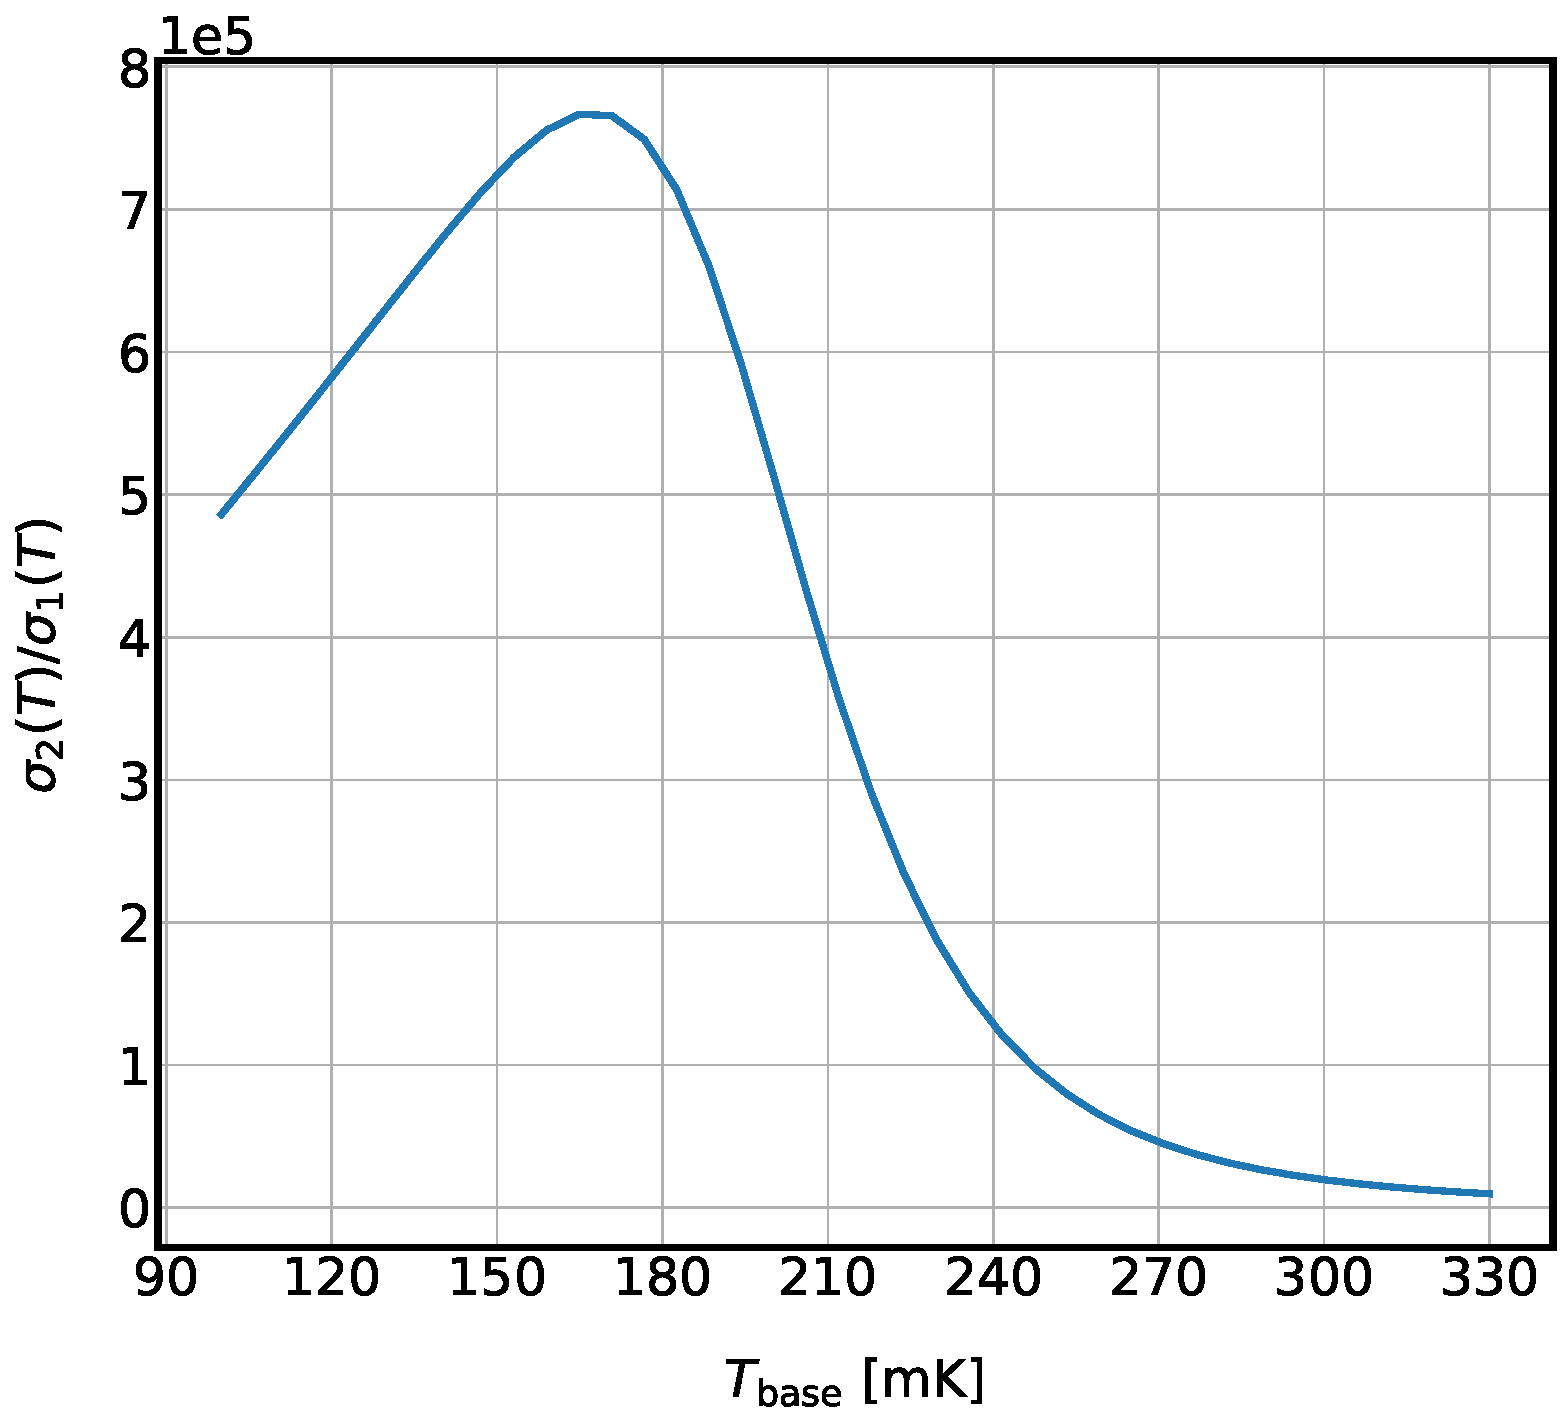
\includegraphics[width=\textwidth]{figures/kid_model/sig_ratio_T}
\caption[~The ratio of \macrocapwrap{\gls{sig1}} to \macrocapwrap{\gls{sig2}} as a function of base temperature.]{The ratio of \gls{sig1} to \gls{sig2} as a function of base temperature.}
\label{fig:sig_ratio_T}
\end{figure}

\begin{figure}[!htbp]
\centering
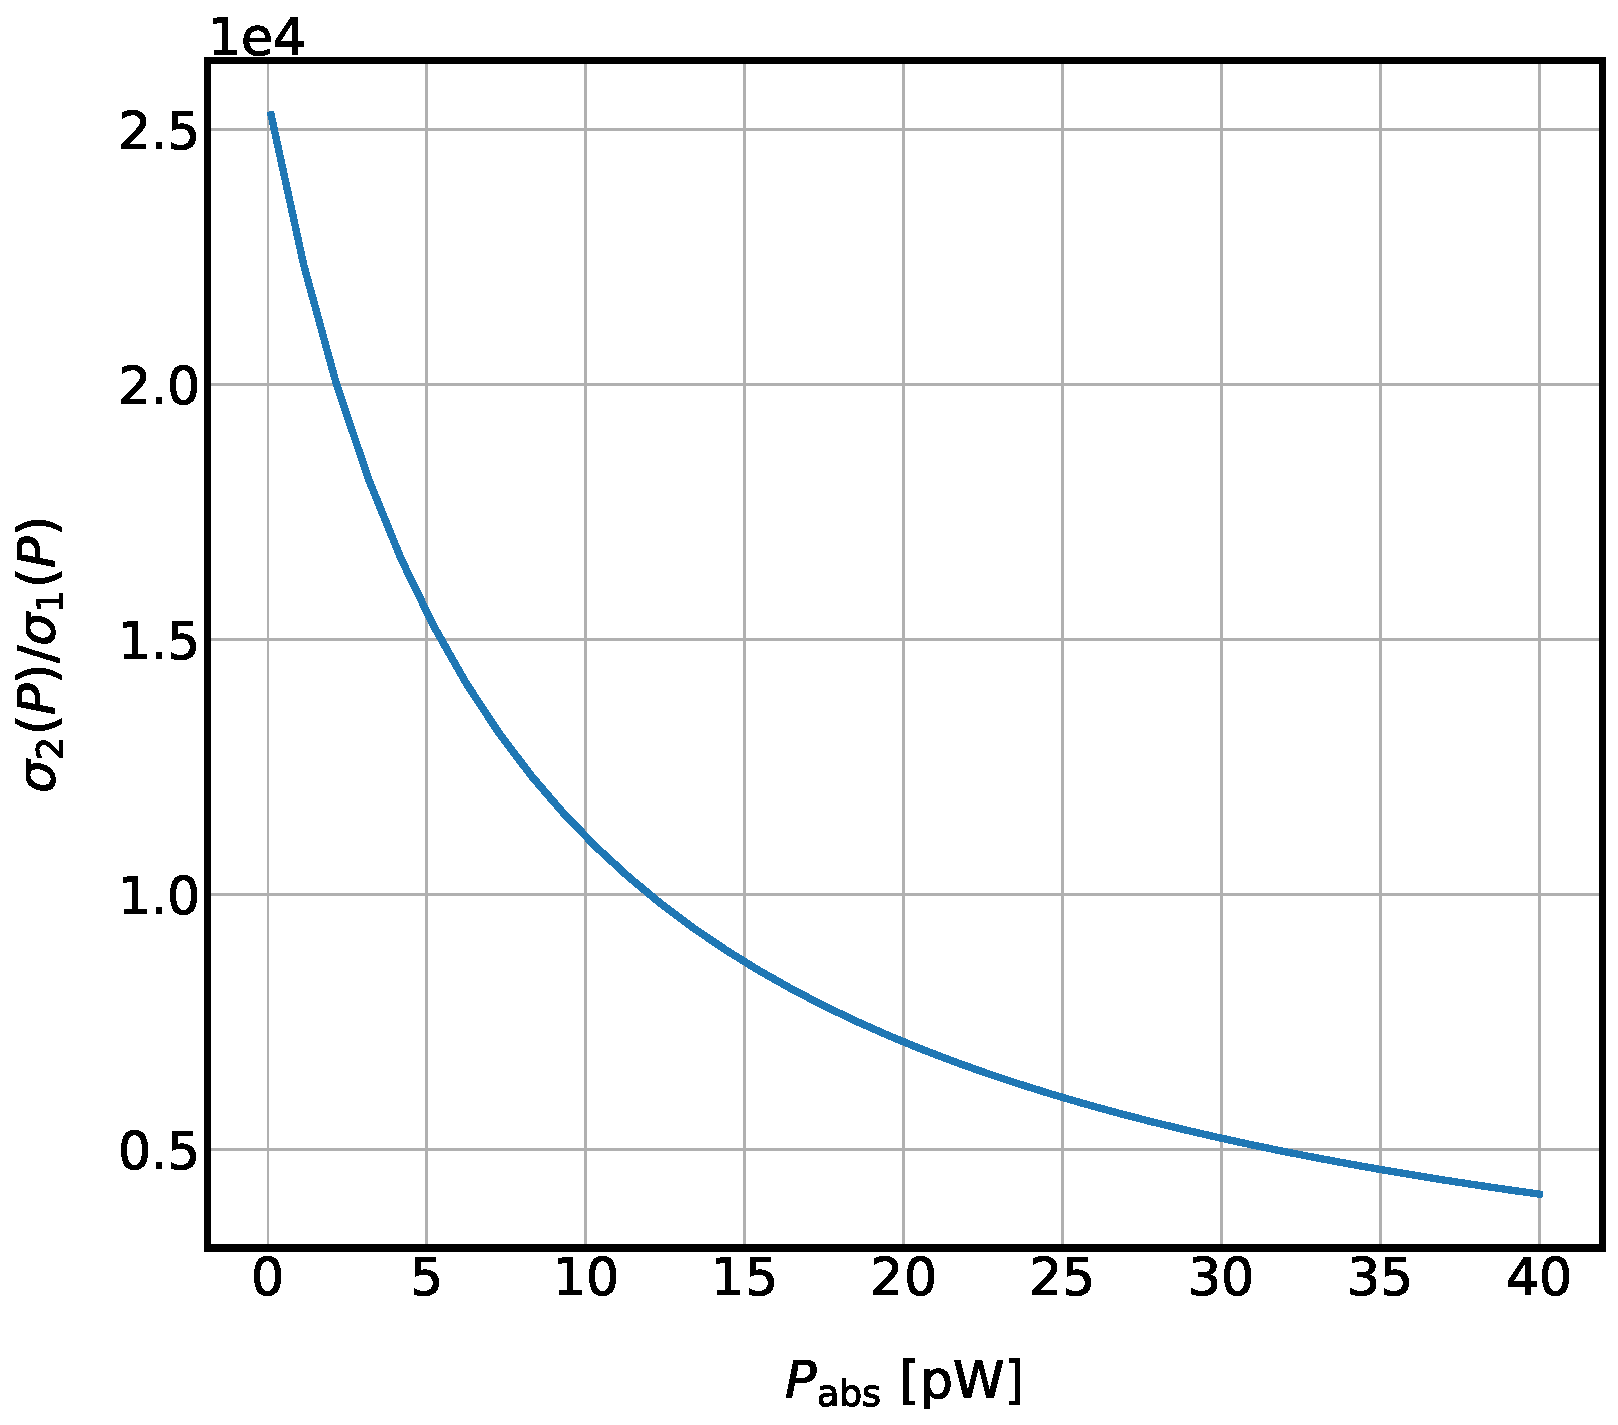
\includegraphics[width=\textwidth]{figures/kid_model/sig_ratio_P}
\caption[~The ratio of \macrocapwrap{\gls{sig1}} to \macrocapwrap{\gls{sig2}} as a function of absorbed optical power at a base temperature of 290~mK.]{The ratio of \macrocapwrap{\gls{sig1}} to \macrocapwrap{\gls{sig2}} as a function of absorbed optical power, at a base temperature of 290~mK.}
\label{fig:sig_ratio_P}
\end{figure}

where $\upmu^{*}$ is an effective chemical potential which is added to the Fermi distribution function to account for QP generation due to pair breaking (for a derivation, see \citet{PhysRevLett.28.1559,gao2008physics}).

% mu thermal
\begin{equation}
  \upmu^{*}_{\mathrm{therm}} = kT\ln\left( \frac{\gls{nqp}}{2\gls{N0}\sqrt 2\pi kT\gls{Delta}} \right) + \gls{Delta}
\end{equation}

% mu optical
\begin{equation}
  \upmu^{*}_{opt} = kT\ln \left( \frac{\gls{Nqp}^{tot}}{2V\gls{N0}\sqrt{2\pi kT\Delta}} \right) + \Delta
\end{equation}

where $\omega$ is the KID resonant frequency, $\gls{sig_n}$ is the normal conductivity of the material, $\xi = \hbar \omega/2kT$, \gls{K0} is the Modified Bessel function of the second kind of order zero, and \gls{I0} is the Modified Bessel function of order zero.

\section{Kinetic Inductance}\label{sec:kinetic_inductance}

When a voltage is applied to a closed circuit, current does not start to flow instantaneously. The reason for this is that some energy from the applied voltage must first be stored in a B-field, via the inductance $L$. Inductance is defined as the ratio of the applied voltage to the rate of change of the current: $L = \frac{V}{dI/dt}$ [$\Omega$/Hz]. The energy stored in the inductance is $E_{L} = \frac{1}{2}LI^{2}$. The magnetic inductance \gls{Lm} of a superconducting film depends solely on its geometric parameters: Length $l$, width $w$, thickness $t$.

In all conductors there is an additional form of inductance, known as the kinetic inductance (KI) $L_{k}$. The total inductance is the sum of the magnetic (or geometric) and kinetic inductances:

% total inductance
\begin{equation}
  L_{\mathrm{tot}} = \gls{Lm} + L_{k}
\end{equation}

It's useful to define a KI fraction, as:

\begin{equation}
  \gls{alphaKI} = \frac{L_{k}}{L_{\mathrm{tot}}}
\end{equation}

The KI arises from the inertia of the CPs. As charge carriers scatter (or break apart, in the case of CPs), the kinetic energy (velocity) of the remaining charge carriers must increase in order to keep the current constant. This increase in velocity cannot happen instantaneously. Therefore, if an AC current is circulated through a superconducting circuit, and the KI is increased, the current undergoes a phase shift. There is a maximum velocity imposed upon the charge carriers, corresponding to the critical, or pair-breaking current of the material, which is described in the Ginzberg-Landau theory (GL) of superconductivity (see Section~\ref{nonlinearKI}) \citep{tinkham2004introduction}.

From an energy standpoint, an expression for the KI can be derived by equating the energy in the KI to the kinetic energy of a CP\@:

\begin{equation}
  \begin{aligned}
  \frac{1}{2}L_{k}I^{2} &= \frac{1}{2}(2m_{e})v_{cp}^{2}N_{cp}\\
                        &= m_{e}^{2}v_{cp}^{2}n_{cp}lA
  \end{aligned}
\end{equation}

where $A = wlt$ is the cross-sectional area of the transmission line (TL), $I_{s}$ is the supercurrent, $v_{cp}$ is the CP velocity and $N_{cp}$ is the total number of CPs. Defining the supercurrent as

\begin{equation}
  \begin{aligned}
  I_{s} = \frac{1}{2}n_{cp}(2e)v_{cp}A
  \end{aligned}
\end{equation}

the KI per unit length is

\begin{equation} \label{eq:KI_per_length}
  \gls{Lk_per_l} = \frac{m_{e}}{n_{cp}e^{2}A}
\end{equation}

The KI can also be understood by considering the impedance. Because CPs are collisionless, their scattering time \gls{tau_s} is infinite. Taking the limit of Equation~\ref{eq:drude} as \gls{tau_s} goes to infinity:

\begin{equation}
    \begin{aligned}
    \lim_{\gls{tau_s} \to \infty} \gls{sig_d}(\omega) &= -j\frac{n_{e}e^{2}}{m_{e}\omega}\\
    &= \gls{sig2}
    \end{aligned}
\end{equation}

Therefore, the KI per unit length is

\begin{equation}
  \gls{Lk_per_l}(\omega) = \frac{1}{\gls{sig2}\omega t}
\end{equation}

and the KI per square is

\begin{equation}
  \gls{Lk_per_sq}(\omega) = \frac{1}{\gls{sig2}\omega t}
\end{equation}

The impedance of the superconducting film can be written as a function of the conductivity:

\begin{equation}\label{eq:Z}
  \begin{aligned}
  Z(\omega) &= \frac{1}{t\sigma(\omega)}\\
            &= \frac{1}{t}\left( \frac{\gls{sig1}}{\gls{sig2}^{2}} - j\gls{sig2}^{-1}\right)\\
            &= \mathcal{R} + j\omega\gls{Lk_per_sq}
  \end{aligned}
\end{equation}

where $\mathcal{R}$ is the resistance per square.

Then,

\begin{equation}
  \gls{Lk_per_sq}(\omega) = \frac{1}{\gls{sig2}\omega t}
\end{equation}

Using the fact that in the low-frequency limit ($\hbar\omega \ll kT$), Mattis-Bardeen (MB) theory allows the complex conductivity to be expressed as (\citet{mauskopf2018transition,annunziata2010tunable}):

\begin{equation}
  \gls{sig2} = \frac{\gls{sig_n}\pi\Delta}{\hbar\omega}\tanh \left(\frac{\gls{Delta}}{2kT}\right)
\end{equation}

and the sheet resistance of the film in the normal state is \gls{Rsq} = 1/\gls{sig_n}t, the KI per square becomes:

\begin{equation} \label{eq:Lk_Rsq}
  \gls{Lk_per_sq}(T,P) = \frac{\hbar\gls{Rsq}}{\pi\Delta(T,P)}
\end{equation}

Equation~\ref{eq:Lk_Rsq} illustrates the fact that materials with higher normal state sheet resistivity, and/or smaller band gaps, have higher intrinsic KI fractions \gls{alphaKI}. Figures~\ref{fig:alpha_T} and~\ref{fig:alpha_P} show \gls{alphaKI} as a function of \gls{Tbase} and \gls{Pabs}. The KI fraction is expontial in \gls{Tbase}, but linear in \gls{Pabs}.

\begin{figure}[!htbp]
\centering
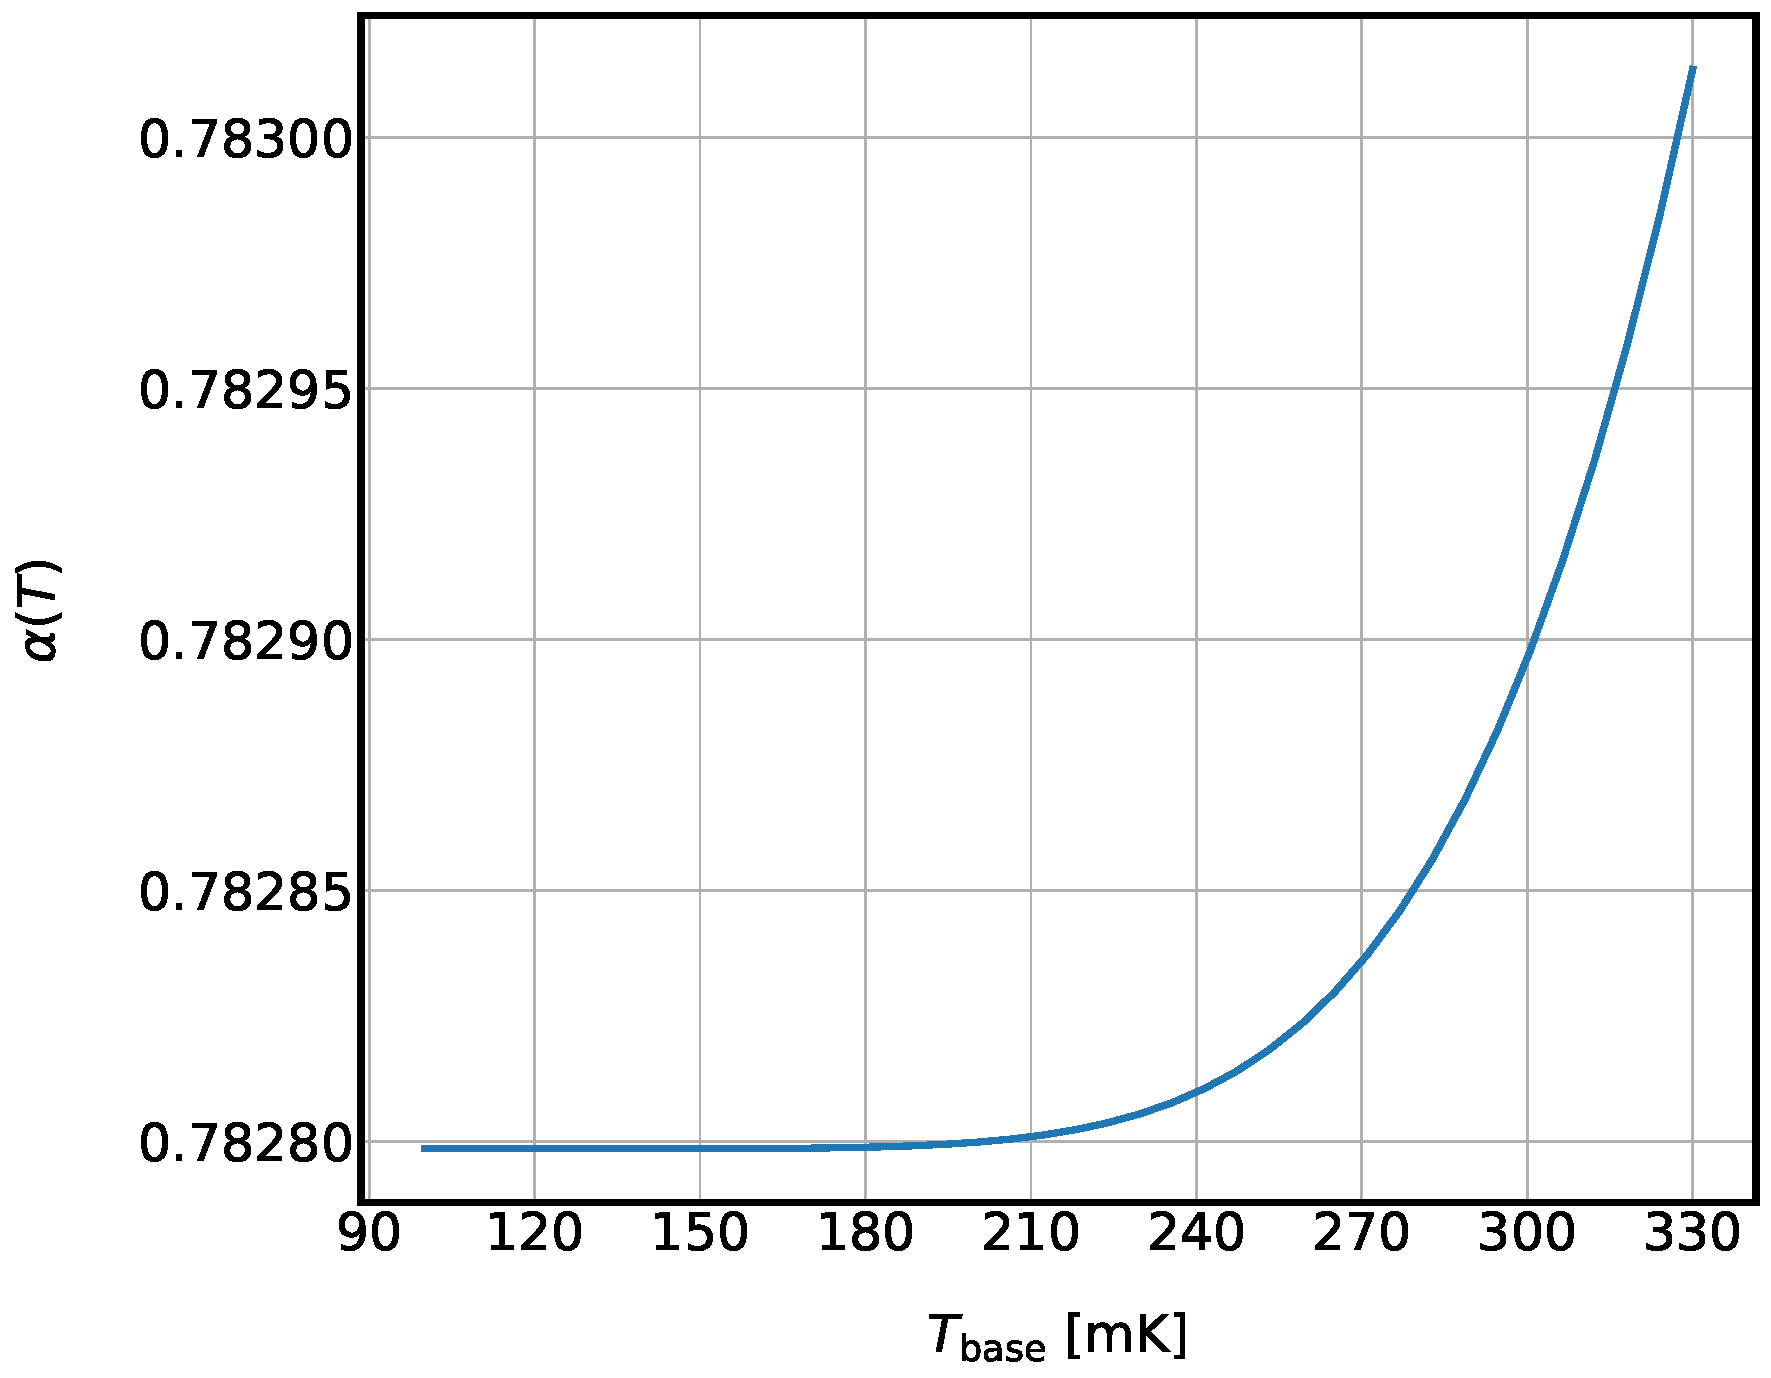
\includegraphics[width=\textwidth]{figures/kid_model/alpha_T}
\caption[~\macrocapwrap{\gls{alphaKI}} as a function of base temperature.]{The kinetic inductance ratio \gls{alphaKI} as a function of base temperature.}
\label{fig:alpha_T}
\end{figure}

\begin{figure}[!htbp]
\centering
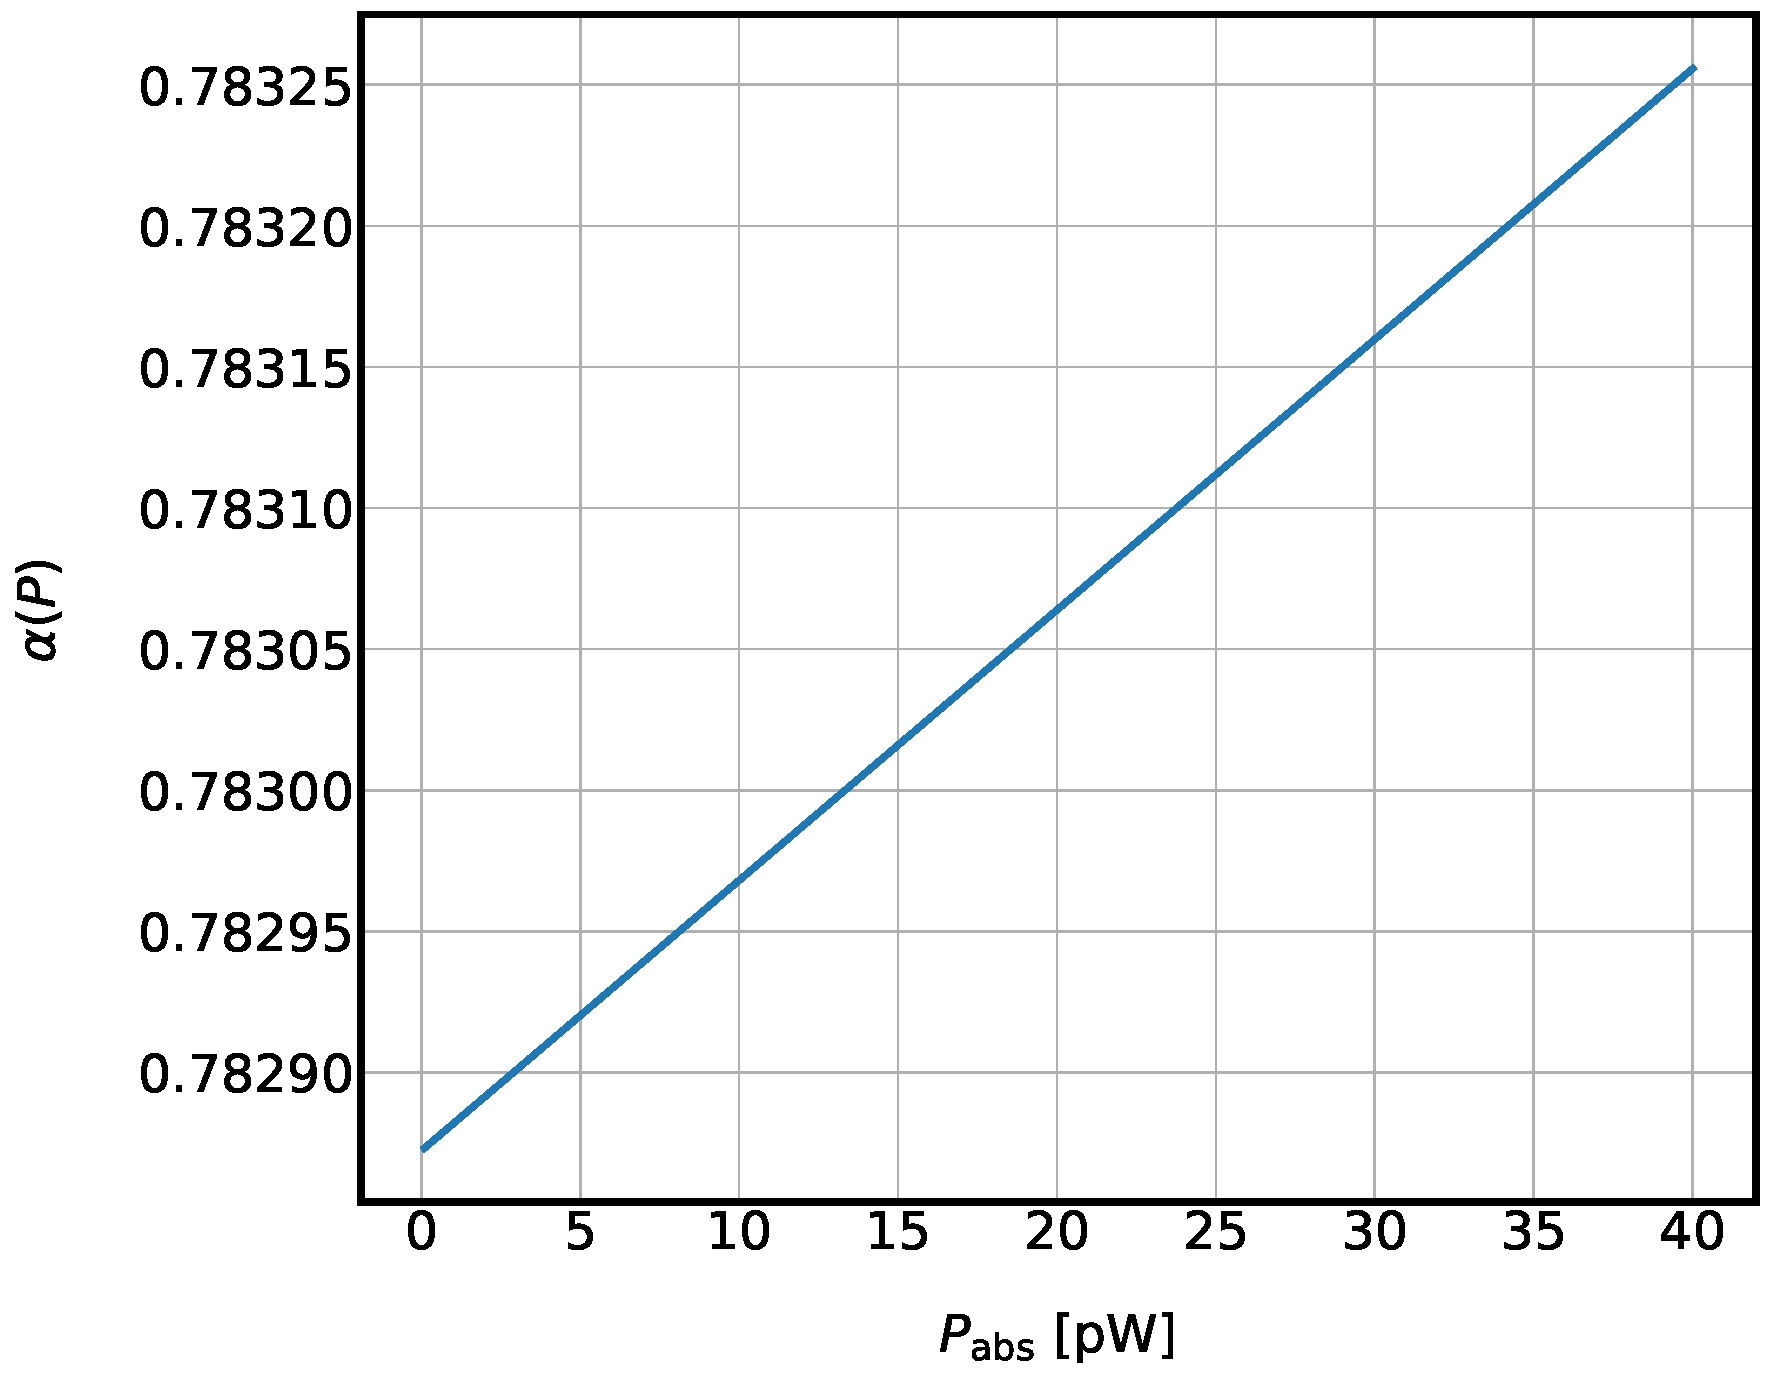
\includegraphics[width=\textwidth]{figures/kid_model/alpha_P}
\caption[~\macrocapwrap{\gls{alphaKI}} as a function of absorbed power.]{The kinetic inductance fraction \gls{alphaKI} as a function of optical power.}
\label{fig:alpha_P}
\end{figure}

\section{Principle LEKID Parameters}\label{sec:kid_params}

In the previous sections, several superconducting device properties were derived as functions of base temperature \gls{Tbase} and absorbed optical power \gls{Pabs}. Now, we introduce a circuit model for a lumped-element KID (LEKID), and derive the temperature and power dependence of several intrinsic and empirical (determined from measurements) parameters.

\subsection{Intrinsic and Empirical Parameters}

A LEKID is a capacitively-coupled lumped-element resonant circuit (tank circuit). It has five intrinsic circuit parameters. These are:

\begin{itemize}[label={},nosep]
  \item $L_{\mathrm{tot}}$ \quad The total resonator inductance
  \item $C_{r}$ \quad The resonator capacitance
  \item $C_{c}$ \quad The coupling capacitance
  \item $R_{\mathrm{eff}}$ \quad An effective resistance, in series with $L_{\mathrm{tot}}$, which accounts for the real part of the resonator impedance
  \item $Z_{0}$ \quad The feedline impedance
\end{itemize}

Figure~\ref{fig:lekid_schematic} shows a schematic which illustrates how a LEKID is constructed from the basic elements listed above.

There are four principle empirical parameters:

\begin{itemize}[label={},nosep]
  \item \gls{Qr} \quad Resonator quality factor
  \item \gls{Qc} \quad Coupling quality factor
  \item $\omega_{0}$ \quad Resonant frequency
  \item \gls{asym} \quad A parameter which accounts for a frequency dependent asymmetry in resonator impedance
\end{itemize}

\begin{figure}[!htbp]
\centering
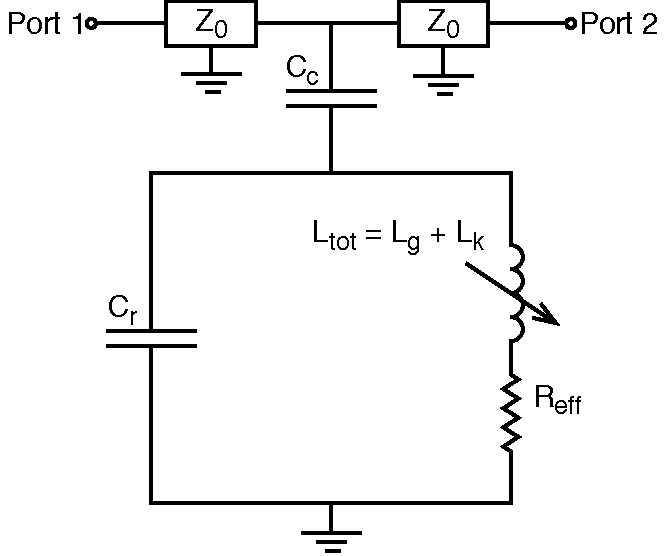
\includegraphics[width=0.5\textwidth]{figures/kid_model/mkid_schematic}
\caption{~A schematic of a single LEKID.}
\label{fig:lekid_schematic}
\end{figure}

The resonant frequency is set by the total inductance and resonator capacitance:

\begin{equation}\label{eq:f0}
  \omega_{0} = \frac{1}{\sqrt{\mathcal{L}_{\mathrm{tot}}\mathcal{C}_{r}}}
\end{equation}

From the perspective of a microwave carrier tone which is input to the feedline at frequency $\omega_{c} = 2\pi f_{c}$, the LEKID acts as a frequency dependent shunt impedance to ground. The resonant frequency of the LEKID is changed by modulating the KI, with a combination of changes in absorbed optical power, base temperature and microwave probe tone power. Taking the derivative of Equation~\ref{eq:f0} with respect to \gls{Lk_per_l}, and defining the resonator capacitance as $C_{r} = \frac{1}{L_{\mathrm{tot}}\omega_{0}^{2}}$,

\begin{equation}
 \frac{df_{0}}{d\gls{Lk_per_l}} = \frac{-\alpha f_{0}}{2\gls{Lk_per_l}}
\end{equation}

The asymmetry parameter is defined as $\gls{asym} = \frac{C_{r}}{C_{c}\gls{Qi}}$
where \gls{Qi} is the internal quality factor \citep{mauskopf2018transition}. The internal quality factor is itself defined as:

% Qi
\begin{equation}\label{eq:Qi}
  \gls{Qi} = \frac{\Im(Z_{r})}{\Re(Z_{r})} = \frac{\omega_{c}L_{\mathrm{tot}}}{R_{\mathrm{eff}}} = \frac{\omega_{c} E_{r}}{P_{\mathrm{diss}}}
\end{equation}

where $E_{r}$ is the stored (internal) energy of the resonator, and $P_{\mathrm{diss}}$ is the dissipated power, or energy dissipated per cycle of the carrier tone at frequency $\omega_{c}$. The couping quality factor is (see \citet{barry2014development}):

\begin{equation} \label{eq:Qc}
  \gls{Qc} = \frac{2(C_{r} + C_{c})}{\omega_{0}C_{c}^{2}Z_{0}}
\end{equation}

The measured resonator quality factor, $Q_{r}$, is related to the internal and coupling quality factors as:
% Qr, measured resonator quality factor
\begin{equation}
  \frac{1}{\gls{Qr}} = \frac{1}{\gls{Qi}} + \frac{1}{\gls{Qc}} + \frac{1}{Q_{\mathrm{loss}}}
\end{equation}

where $Q_{\mathrm{loss}}$ is an external loss factor, typically of $\mathcal{O}(10^{6})$, which accounts for parasitic loss, including parasitic capacitance and inductance.

Figures~\ref{fig:Qr_T} and~\ref{fig:Qr_P} show \gls{Qr} as a function of \gls{Tbase} and \gls{Pabs}. While $\gls{Qr}(P)$ decreases monotonically with increasing absorbed optical power, $\gls{Qr}(T)$ does not. Starting at $\gls{Tbase} = 90$~mK, $\gls{Qr}(T)$ first increases with base temperature, reaching a maximum at $\gls{Tbase} \sim 180$~mK, before decreasing almost linearly.

\begin{figure}[!htbp]
\centering
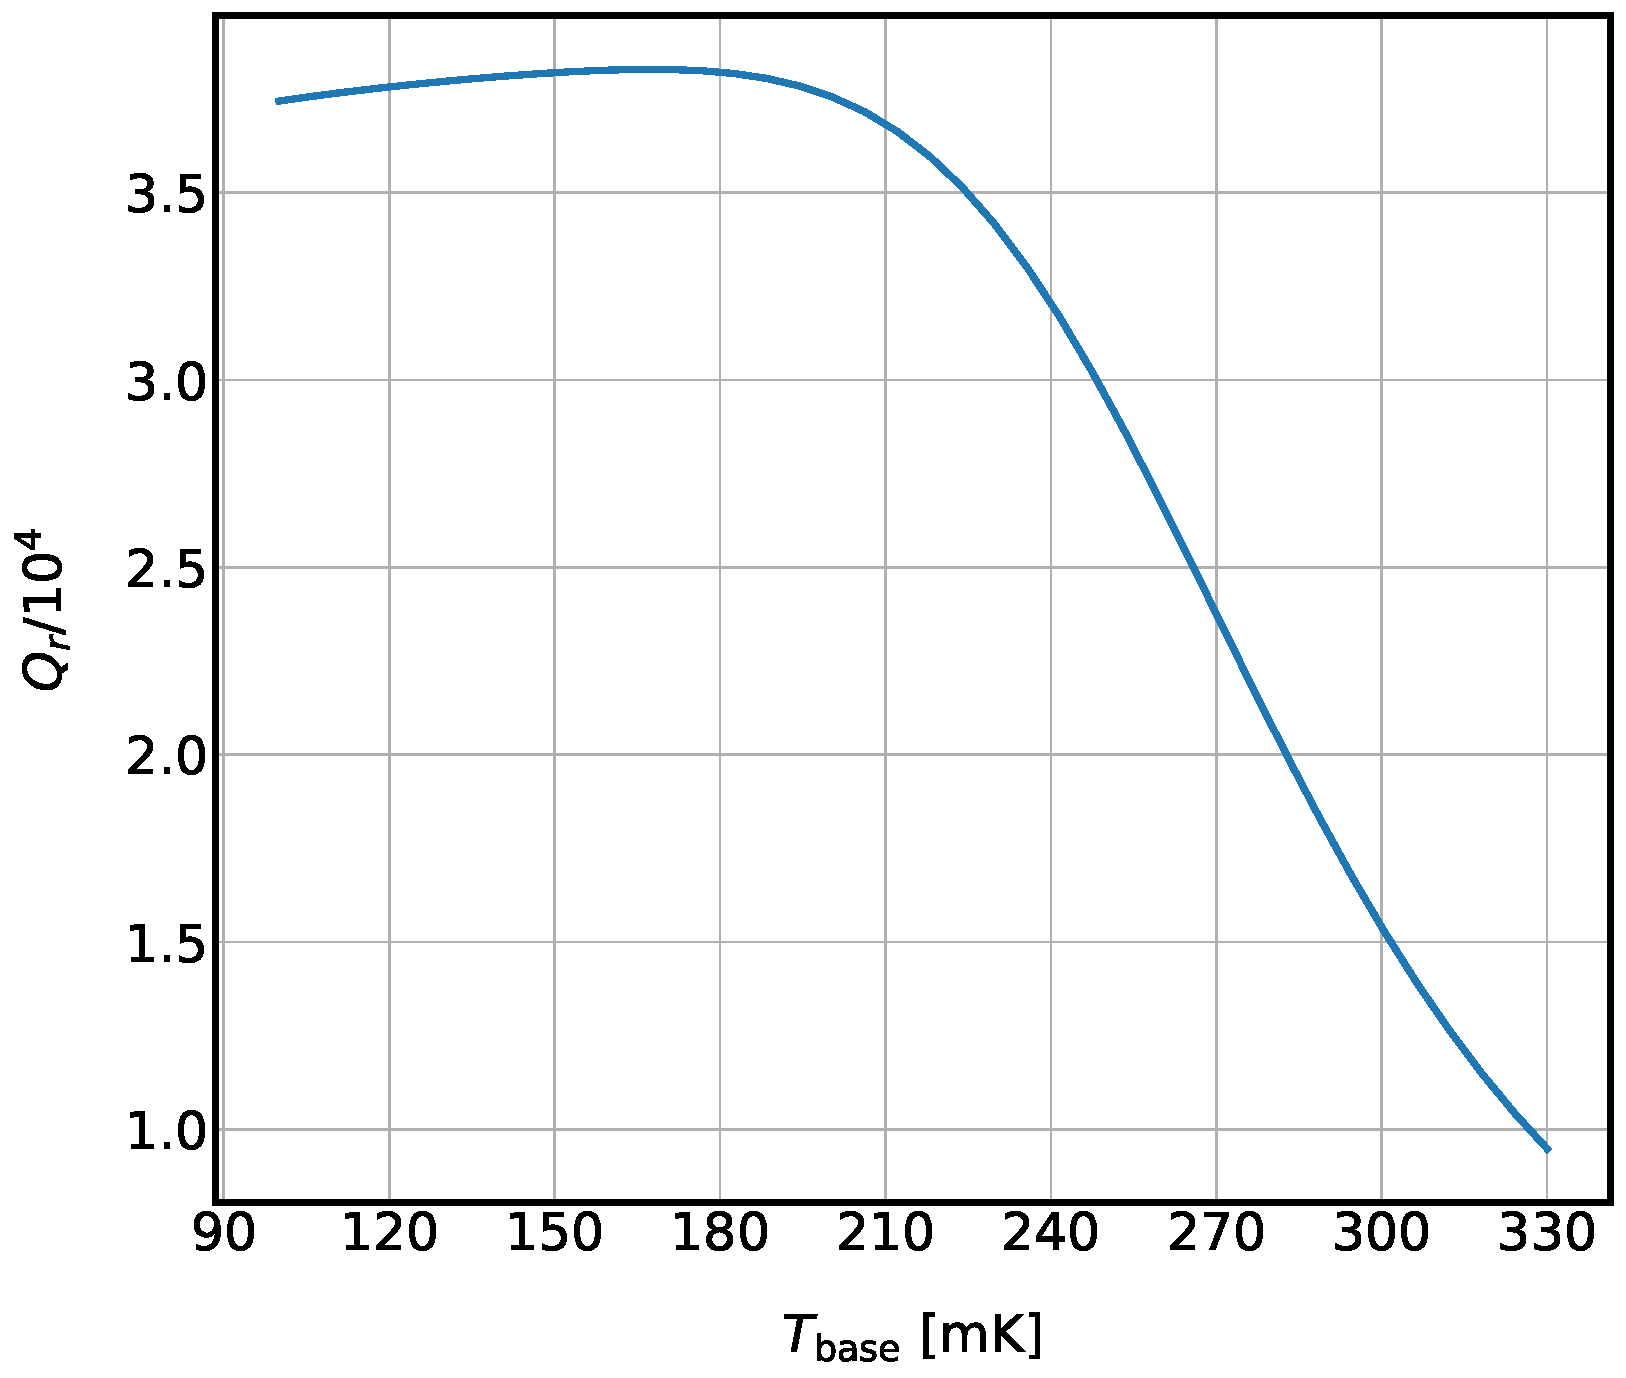
\includegraphics[width=\textwidth]{figures/kid_model/Qr_v_T}
\caption[~Simulated \macrocapwrap{$Q_{r}$} as a function of base temperature.]{Simulated $Q_{r}$ as a function of base temperature.}
\label{fig:Qr_T}
\end{figure}

\begin{figure}[!htbp]
\centering
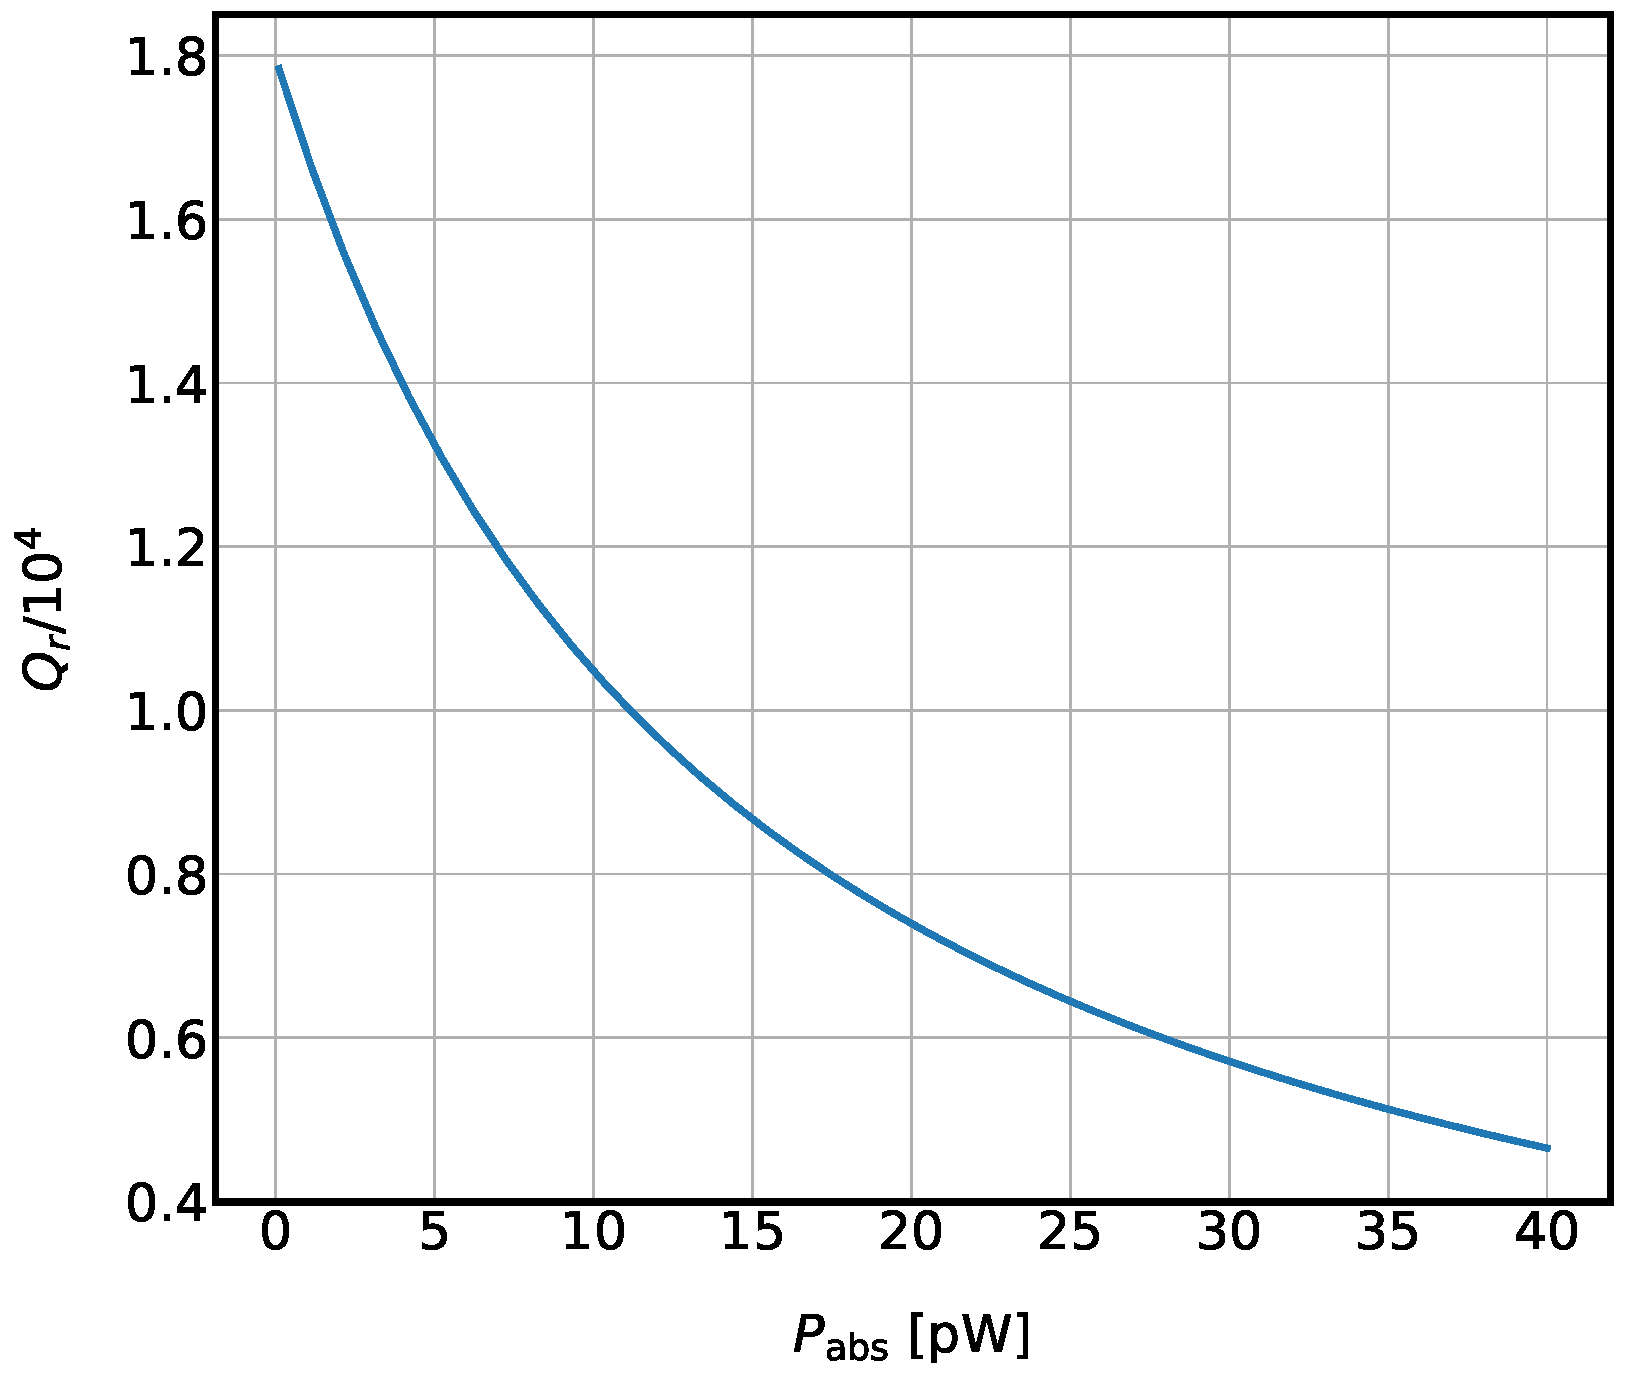
\includegraphics[width=\textwidth]{figures/kid_model/Qr_v_P}
\caption[~Simulated \macrocapwrap{$Q_{r}$} as a function of optical power.]{Simulated $Q_{r}$ as a function of optical power.}
\label{fig:Qr_P}
\end{figure}

\begin{comment}
\begin{figure}[!htbp]
\centering
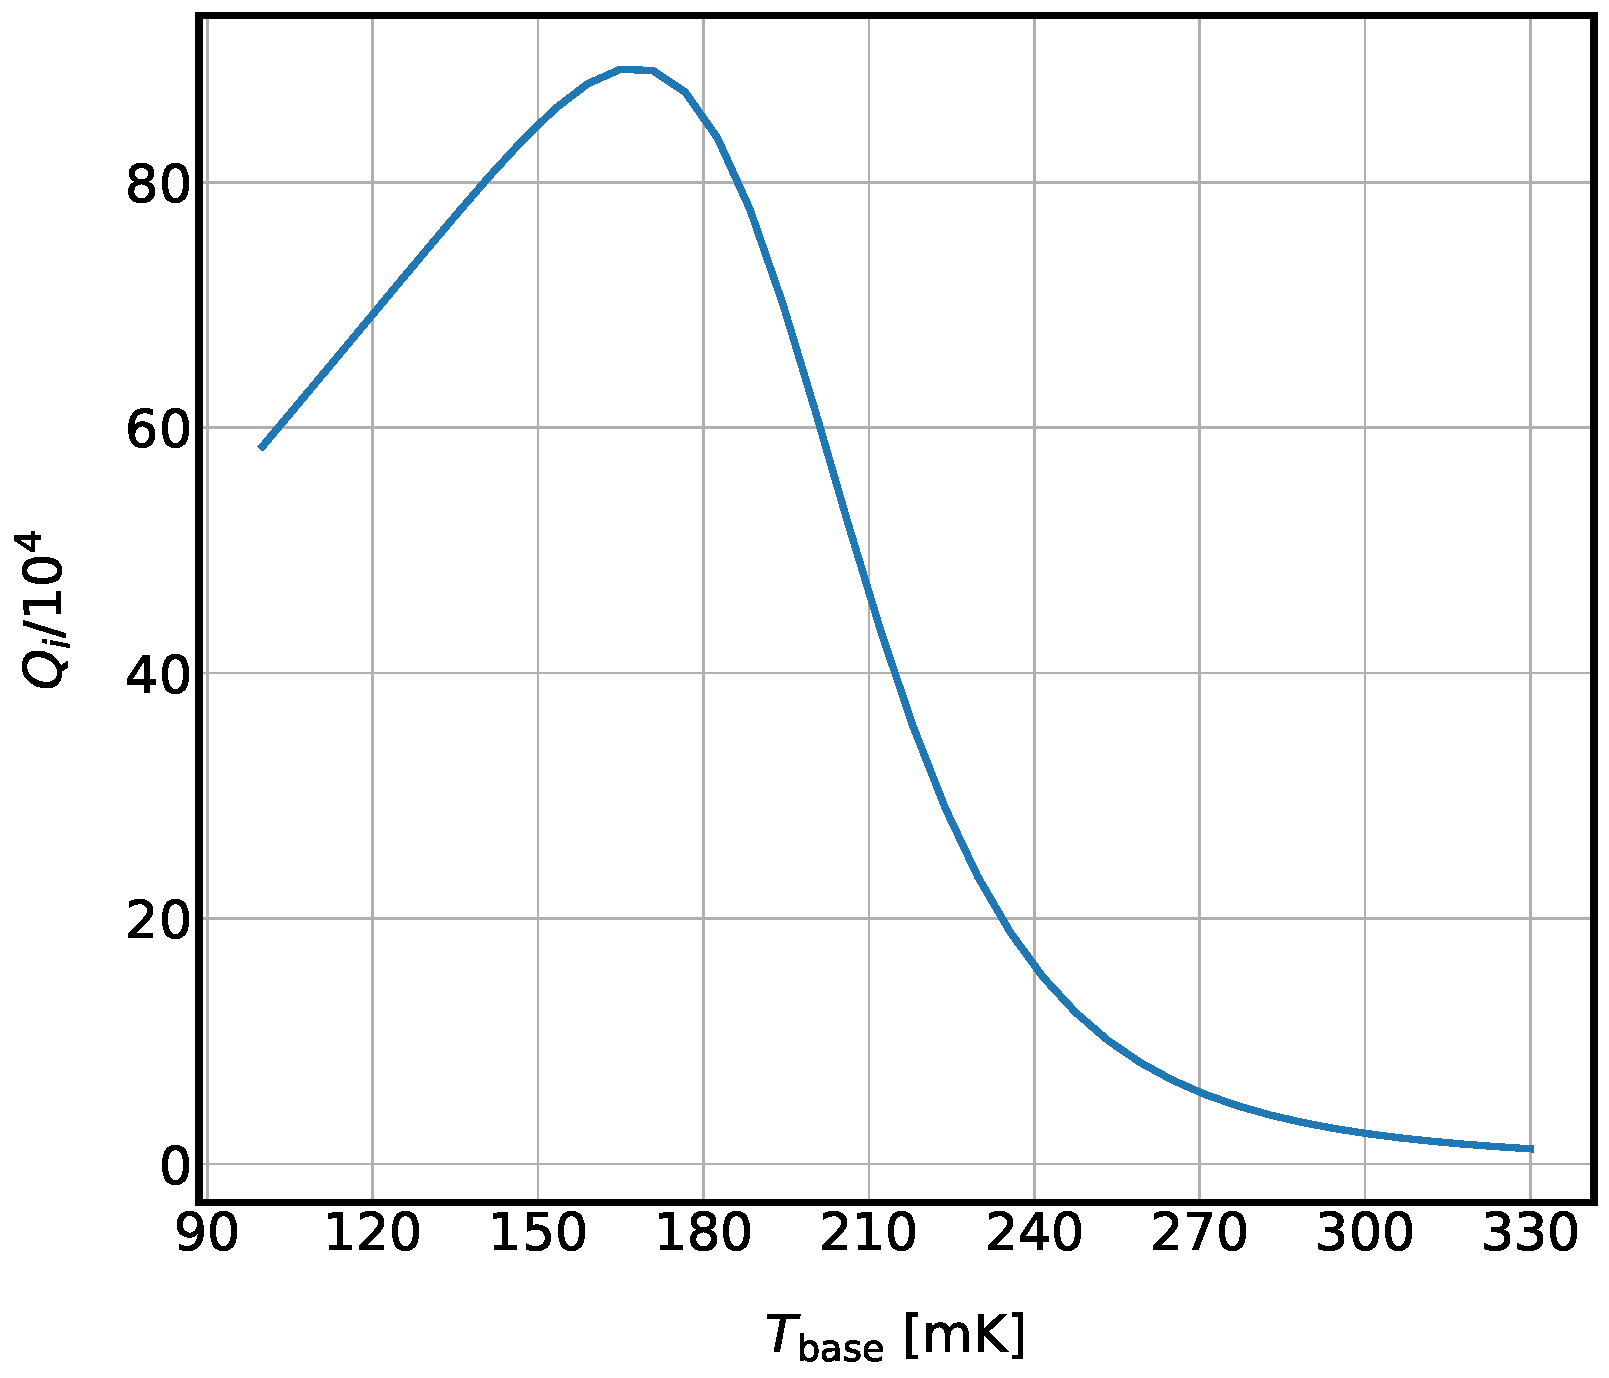
\includegraphics[width=\textwidth]{figures/kid_model/Qi_v_T}
\caption[~Simulated \macrocapwrap{\gls{Qi}} as a function of base temperature.]{Simulated \gls{Qi} as a function of base temperature.}
\label{fig:Qi_T}
\end{figure}

\begin{figure}[!htbp]
\centering
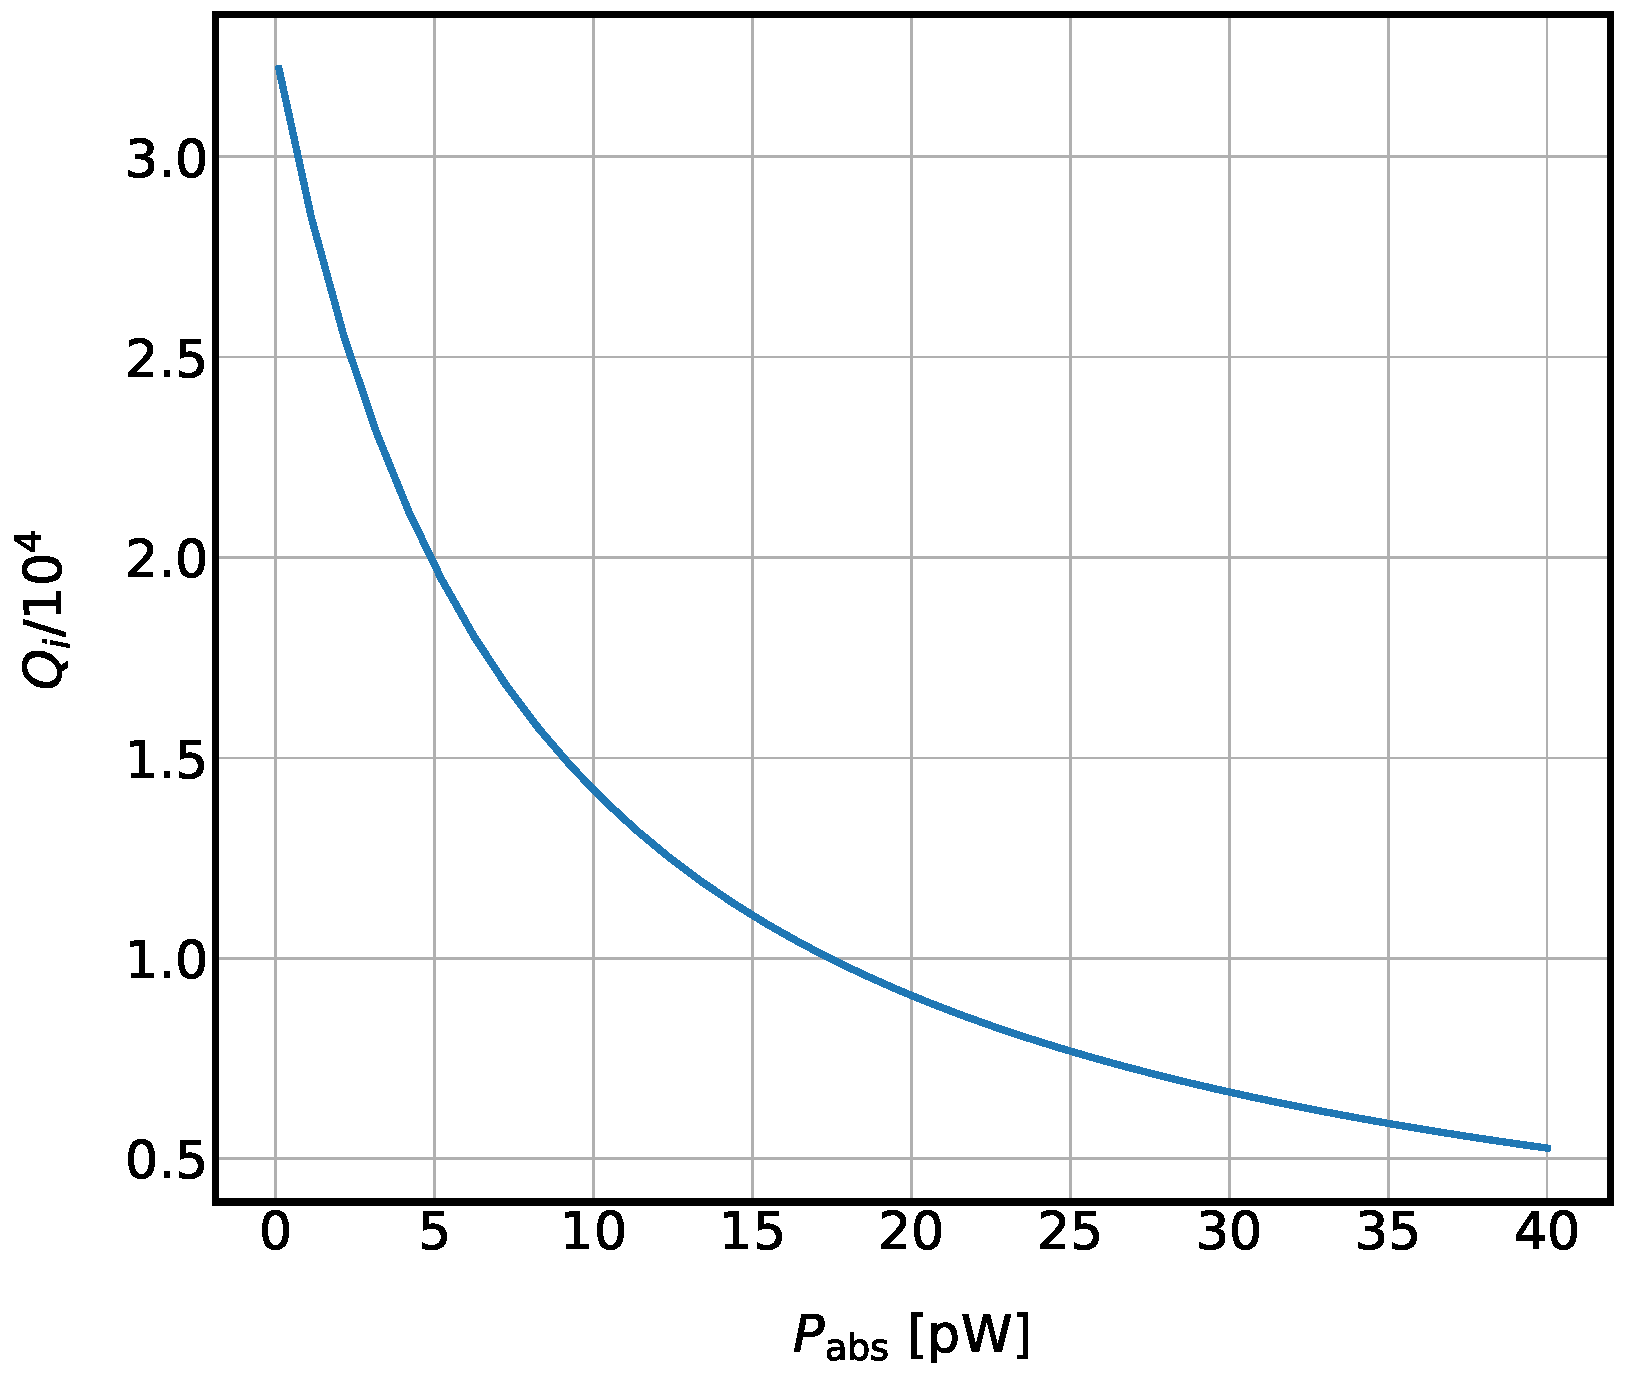
\includegraphics[width=\textwidth]{figures/kid_model/Qi_v_P}
\caption[~Simulated \macrocapwrap{\gls{Qi}} as a function of absorbed optical power.]{Simulated \gls{Qi} as a function of absorbed optical power.}
\label{fig:Qi_P}
\end{figure}
\end{comment}

The empirically determined resonator parameters are determined by measuring the phase and amplitude of the carrier tone after it passes through the LEKID circuit. The resonator impedance  $Z_{r}$ has a frequency dependence which can be expressed as:

\begin{equation}
  Z_{r}(\omega) \simeq Z_{0}\Bigg[ \frac{\gls{Qc}}{2\gls{Qi}} + j\gls{Qc}\delta x \Bigg] \frac{1}{1 + j\gls{asym}}
\end{equation}

where $\delta x = \frac{\omega - \omega_{0}}{\omega_{0}}$. The forward transmission coefficient, $S_{21}$, of the carrier tone expressed as a function of frequency, base temperature and optical power (the dependence of the latter two parameters is implicit) is:

\begin{equation}\label{eq:S21_Z}
  \begin{aligned}
  S_{21}(\omega, T, P) &= 1 - \frac{1}{1 + 2Z_{r}/Z_{0}} \\
                 &= 1 - \frac{1 + j\gls{asym}}{1 + j\gls{asym} \frac{\gls{Qr}}{\gls{Qc}}}\frac{\gls{Qr}}{\gls{Qc}}\Bigg[ \frac{1}{1 + 2j\gls{Qr}\delta x / ( 1 + j\gls{asym}\frac{Qr}{Qc}) }  \Bigg]
  \end{aligned}
\end{equation}

for $\gls{asym} \ll 1$, this reduces to:

\begin{equation}\label{eq:S21}
  S_{21}(\omega, T, P) \simeq 1 - \frac{\gls{Qr}}{\gls{Qc}}\frac{1}{1 + 2j\gls{Qr}\delta x}
\end{equation}

\begin{figure}[!htbp]
  \centering
  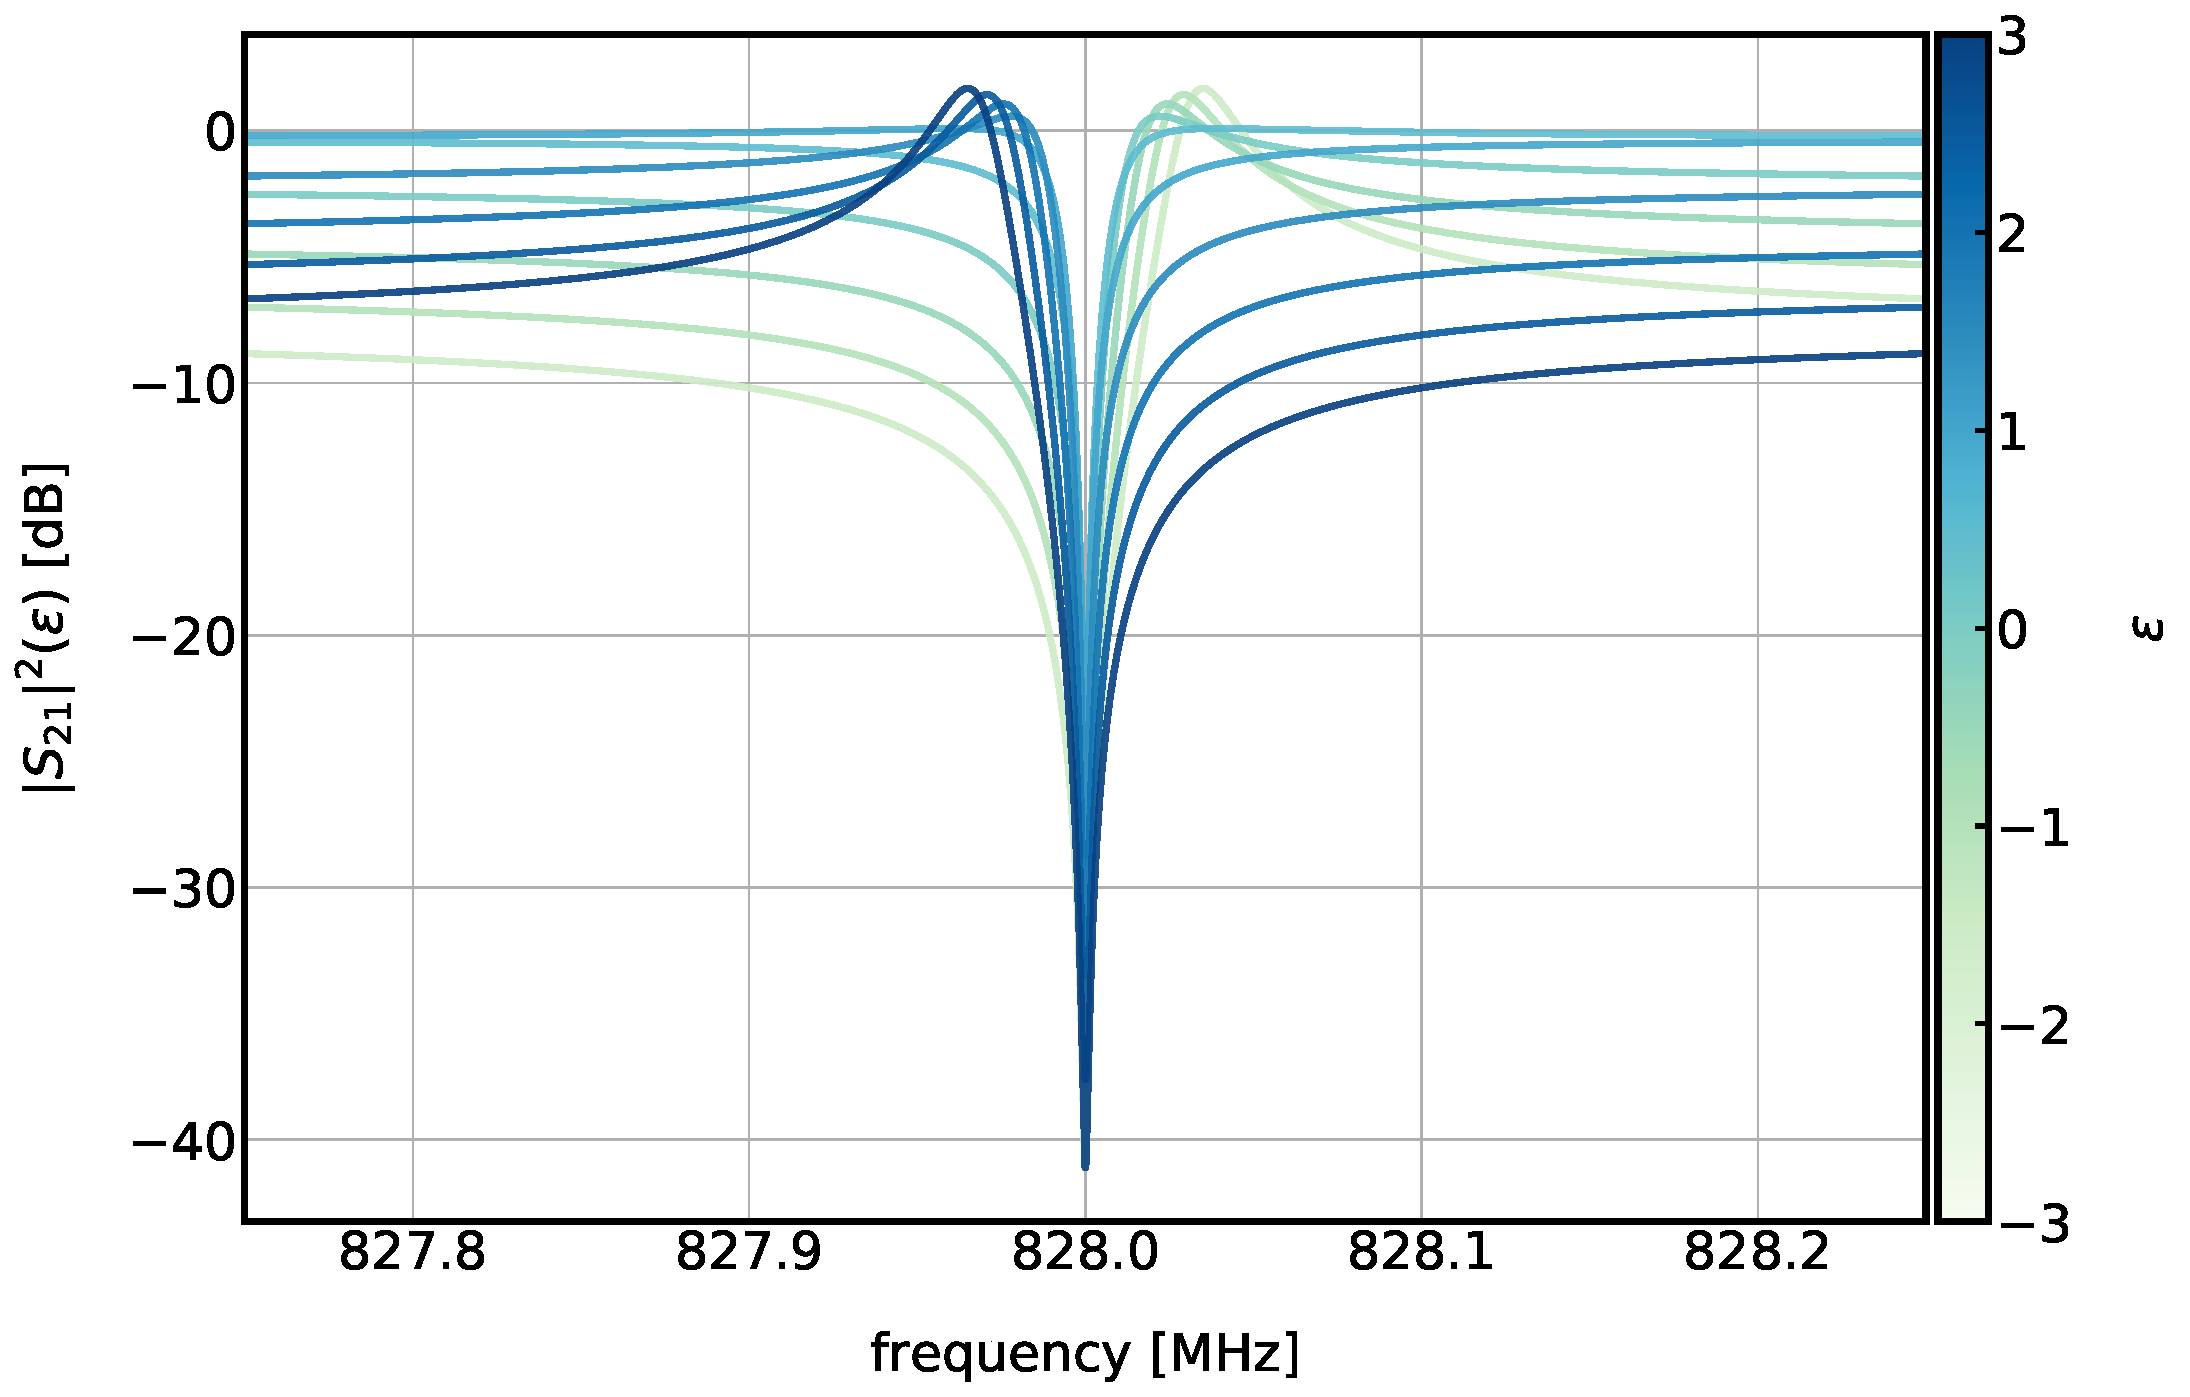
\includegraphics[width=\textwidth]{figures/kid_model/S21_eps}
  \caption[~\macrocapwrap{|\gls{S21}|($\omega$)} for a range of asymmetry parameters.]{$\left| S_{21} \right|(\omega)$ shown for a range of \gls{asym}.}
\label{fig:S21_eps}
\end{figure}

\begin{figure}[!htbp]
  \centering
  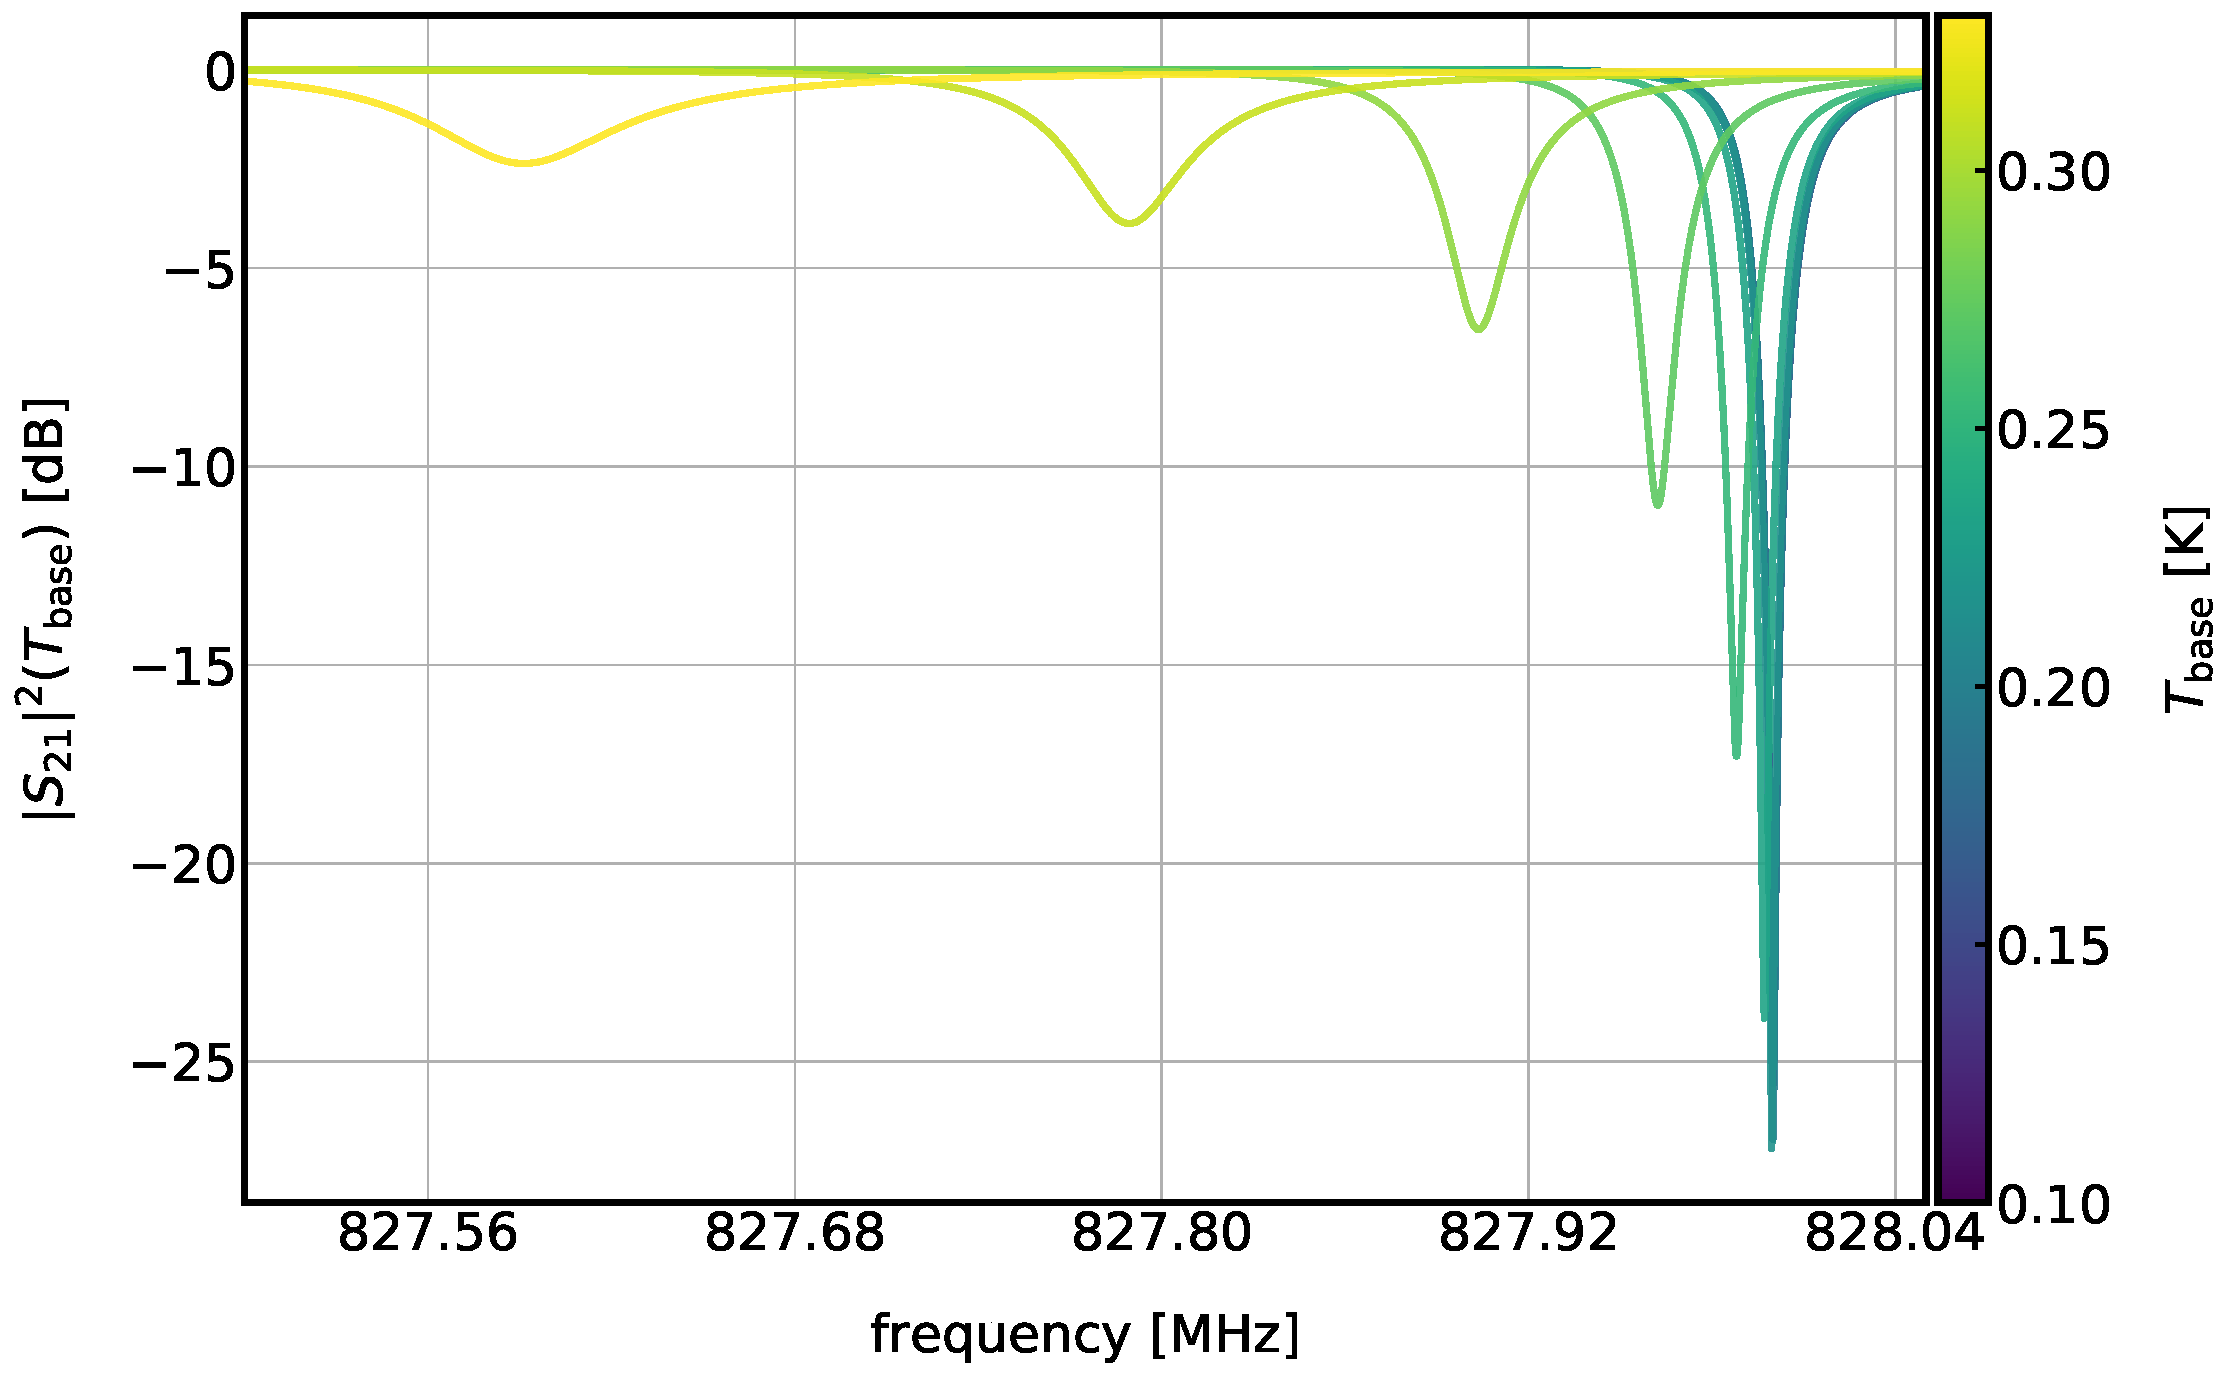
\includegraphics[width=\textwidth]{figures/kid_model/S21_T250}
  \caption[~Simulated \macrocapwrap{|\gls{S21}|($\omega$)} as a function of base temperature.]{Simulated |\gls{S21}|($\omega$) as a function of base temperature.}
\label{fig:S21_T}
\end{figure}

\begin{figure}[!htbp]
  \centering
  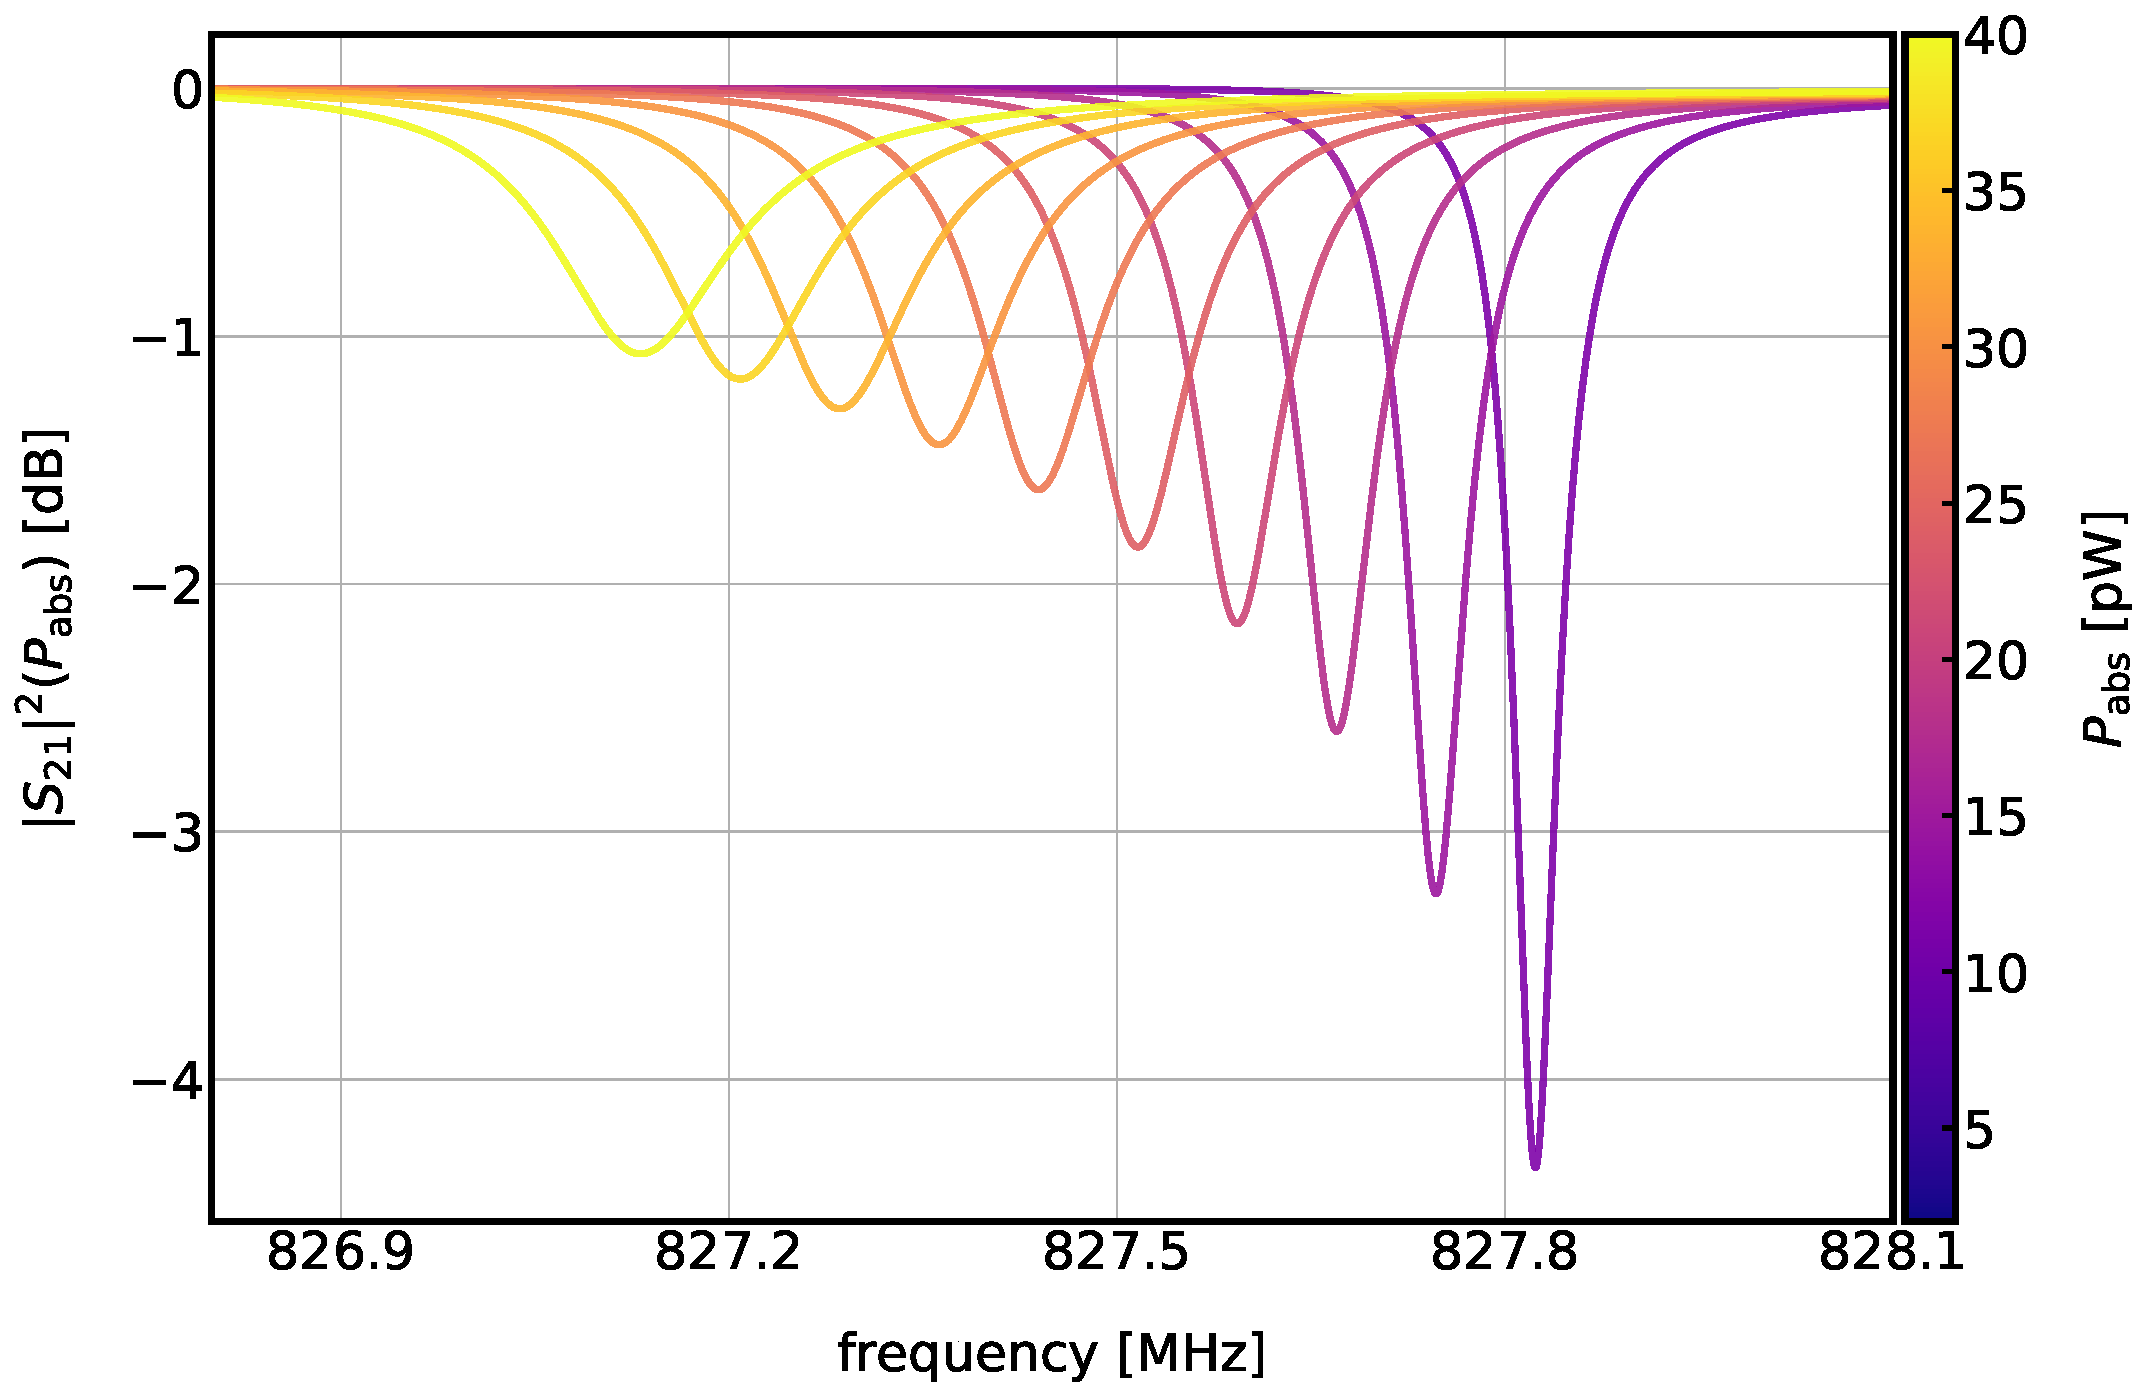
\includegraphics[width=\textwidth]{figures/kid_model/S21_opt250}
  \caption[~Simulated \macrocapwrap{|\gls{S21}|($\omega$)} as a function of optical power.]{Simulated |\gls{S21}|($\omega$) as a function of optical power.}
\label{fig:S21_opt}
\end{figure}

\begin{figure}[!htbp]
  \centering
  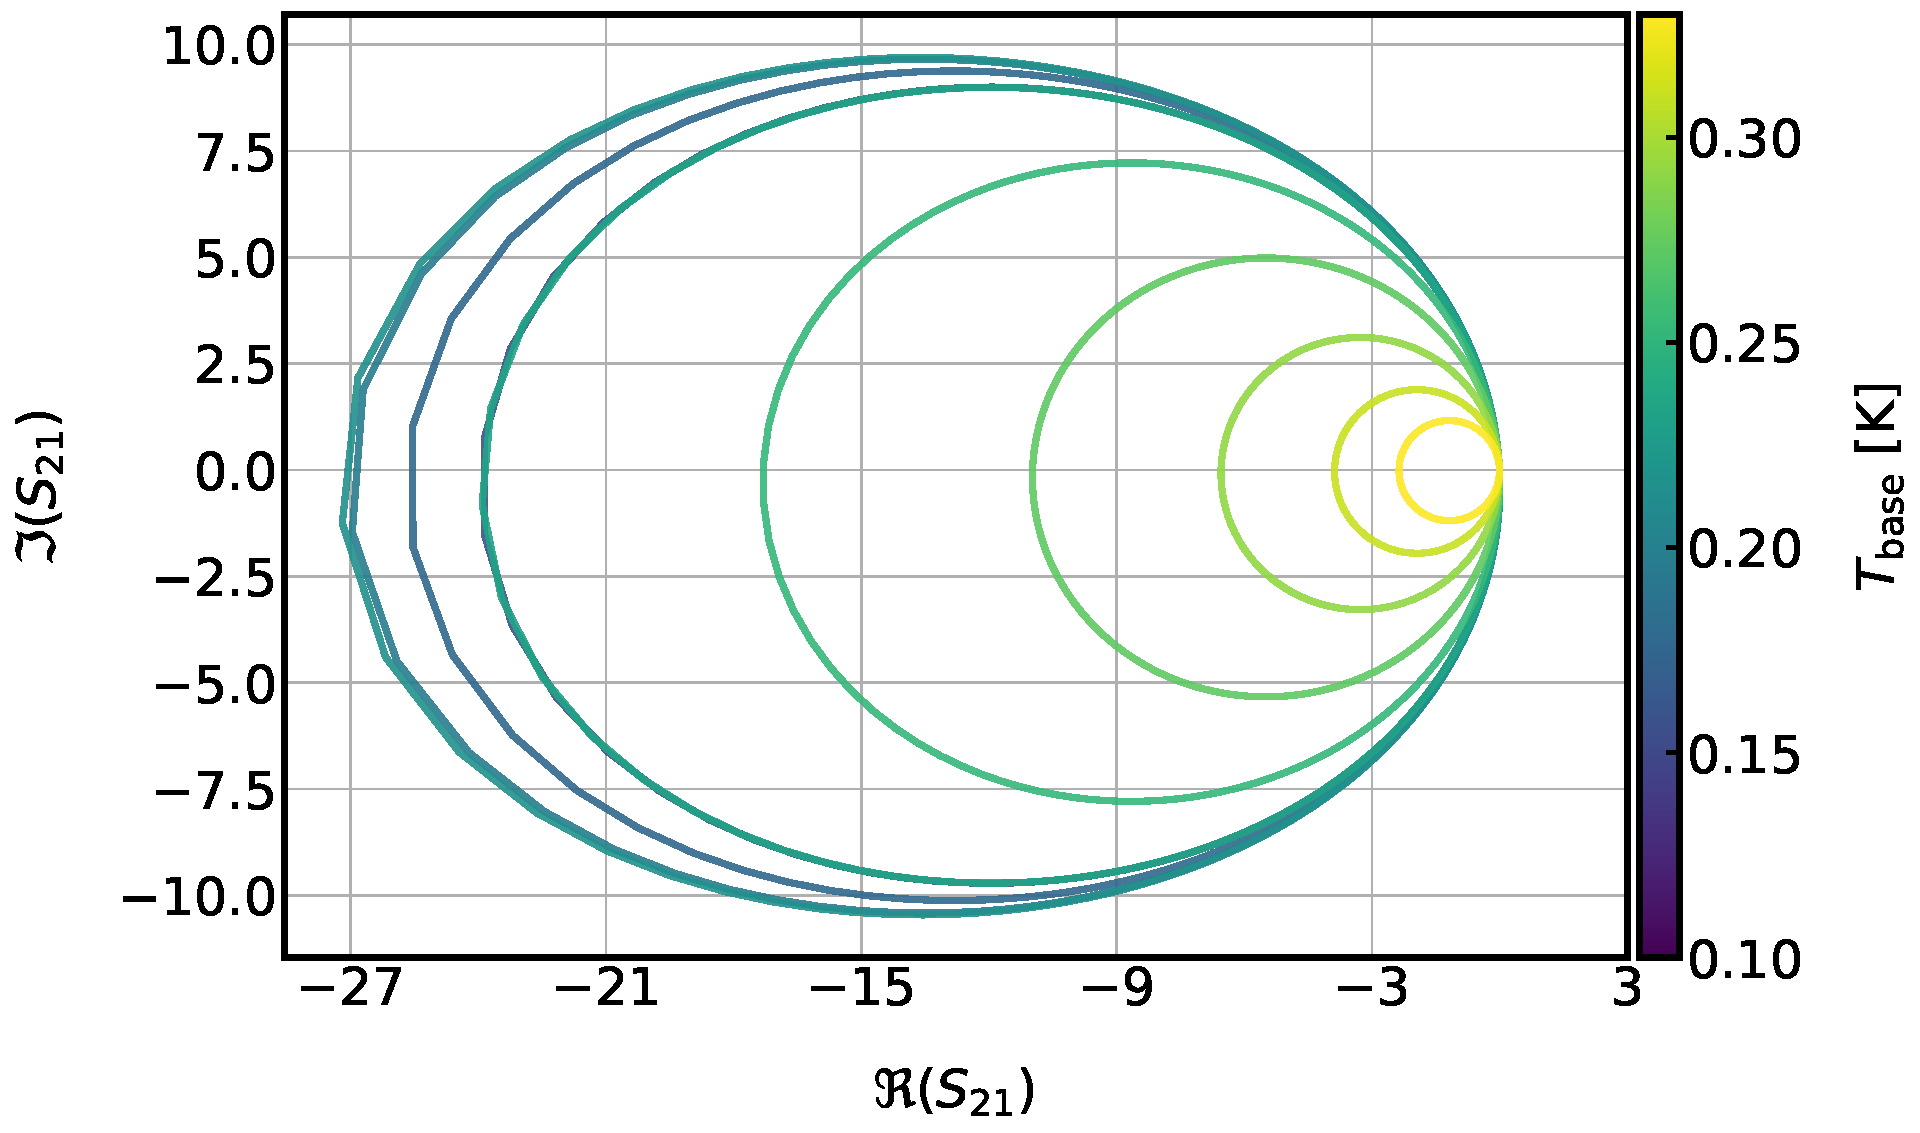
\includegraphics[width=\textwidth]{figures/kid_model/IQloop_T250}
  \caption[~The simulated \macrocapwrap{$I/Q$} loop as a function of base temperature.]{The simulated $I/Q$ loop as a function of base temperature.}
  \label{fig:IQloop_T}
\end{figure}

\begin{figure}[!htbp]
  \centering
  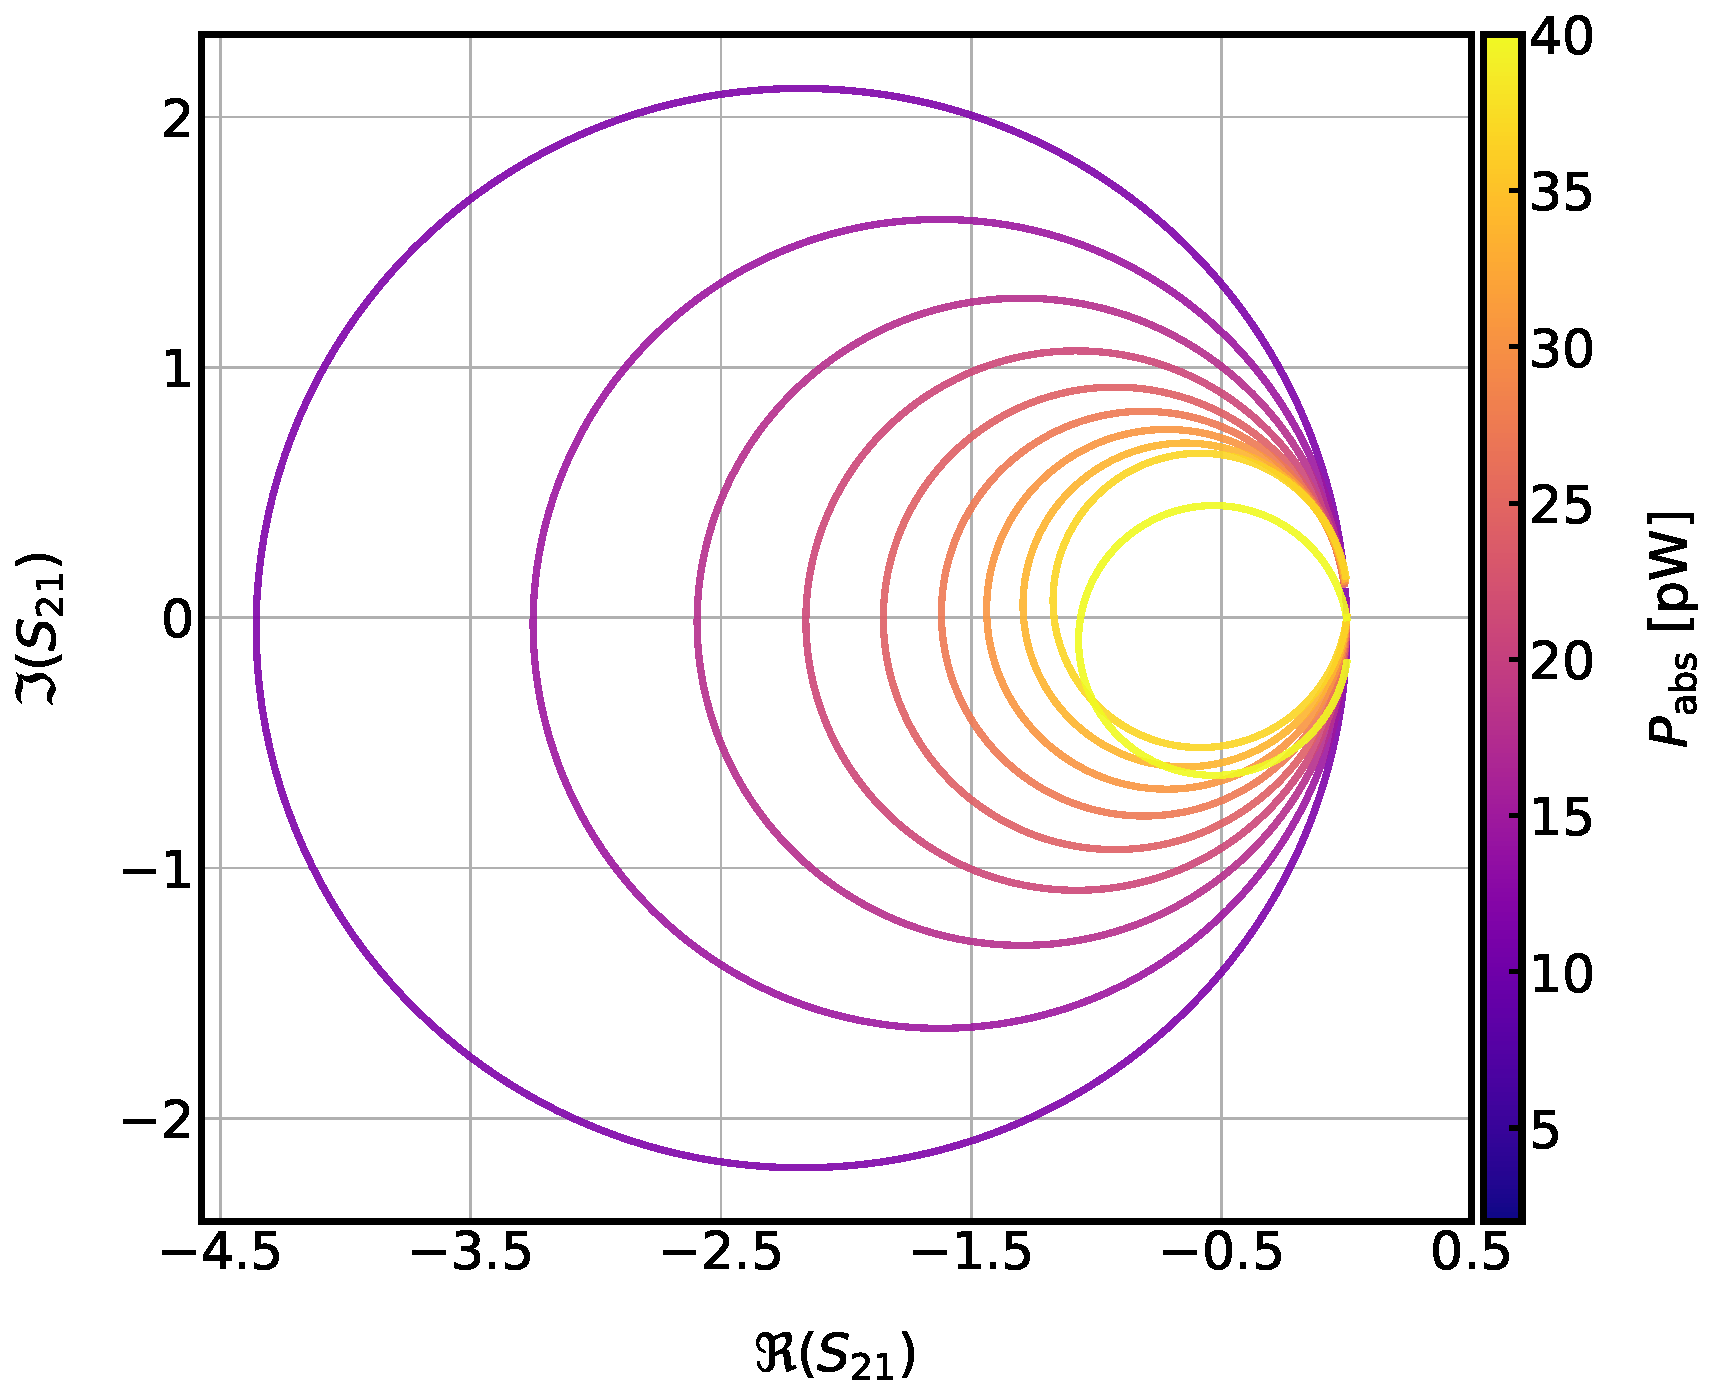
\includegraphics[width=\textwidth]{figures/kid_model/IQloop_opt250}
  \caption[~The simulated \macrocapwrap{$I/Q$} loop as a function of optical power.]{The $I/Q$ loop as a function of optical power.}
\label{fig:IQloop_P}
\end{figure}

Figure~\ref{fig:S21_eps} shows an example $\left| S_{21} \right|(\omega)$ for a wide range (-3--3) of \gls{asym} values. The temperature and power dependence of \gls{S21} are shown in Figures~\ref{fig:S21_T} and~\ref{fig:S21_opt}, for a simulated BLAST-TNG 250~$\upmu$m resonator with $\omega_{0} = 828$~MHz. The `dip-depth' of the \gls{S21} traces is a function of the quality factors:

% dip depth
\begin{equation}\label{eq:dip_depth}
  D = 20\log_{10}\left( 1 - \frac{\gls{Qr}}{\gls{Qc}}\right)
\end{equation}

The `$I/Q$' loops corresponding to Figures~\ref{fig:S21_T} and~\ref{fig:S21_opt} are shown in Figures~\ref{fig:IQloop_T} and~\ref{fig:IQloop_P}, where $I = \Re(\gls{S21})$ and $Q = \Im(\gls{S21})$.

\section{Responsivities}\label{sec:responsivity}

In this section, we derive the LEKID responsivity to fluctuations in base temperature \gls{Tbase} and absorbed optical power \gls{Pabs}.

\subsection{Temperature Responsivity}

The change in the LEKID's resonant frequency in response to a change in base temperature can be written as:

\begin{equation}\label{eq:RT}
  \begin{aligned}
  \gls{Rtemp} &= \frac{df_{0}}{dT} \\
              &= \frac{df_{0}}{d\gls{sig2}} \frac{d\gls{sig2}}{d\gls{nqp}} \frac{d\gls{nqp}}{dT}
  \end{aligned}
\end{equation}

where:

\begin{equation}\label{eq:df0_dsig2}
  \frac{df_{0}}{d\gls{sig2}} = \frac{\alpha f_{0}}{2\gls{sig2}}
\end{equation}

and for $\gls{Tbase} \ll \gls{Tc}$,

\begin{equation}\label{eq:dnqp_dT}
  \frac{d\gls{nqp}}{dT} \simeq \frac{\gls{nqp}}{T} \left(\frac{1}{2} + \frac{\gls{Delta}}{kT} \right)
\end{equation}

Derivations of Equations~\ref{eq:df0_dsig2} and~\ref{eq:dnqp_dT} can be found in \citet{mauskopf2018transition}.

Equation~\ref{eq:RT} is shown graphically in Figure~\ref{fig:dfdT}. It can be seen that \gls{Rtemp} decreases monotonically with increasing \gls{Tbase}.

\begin{figure}[!htbp]
\centering
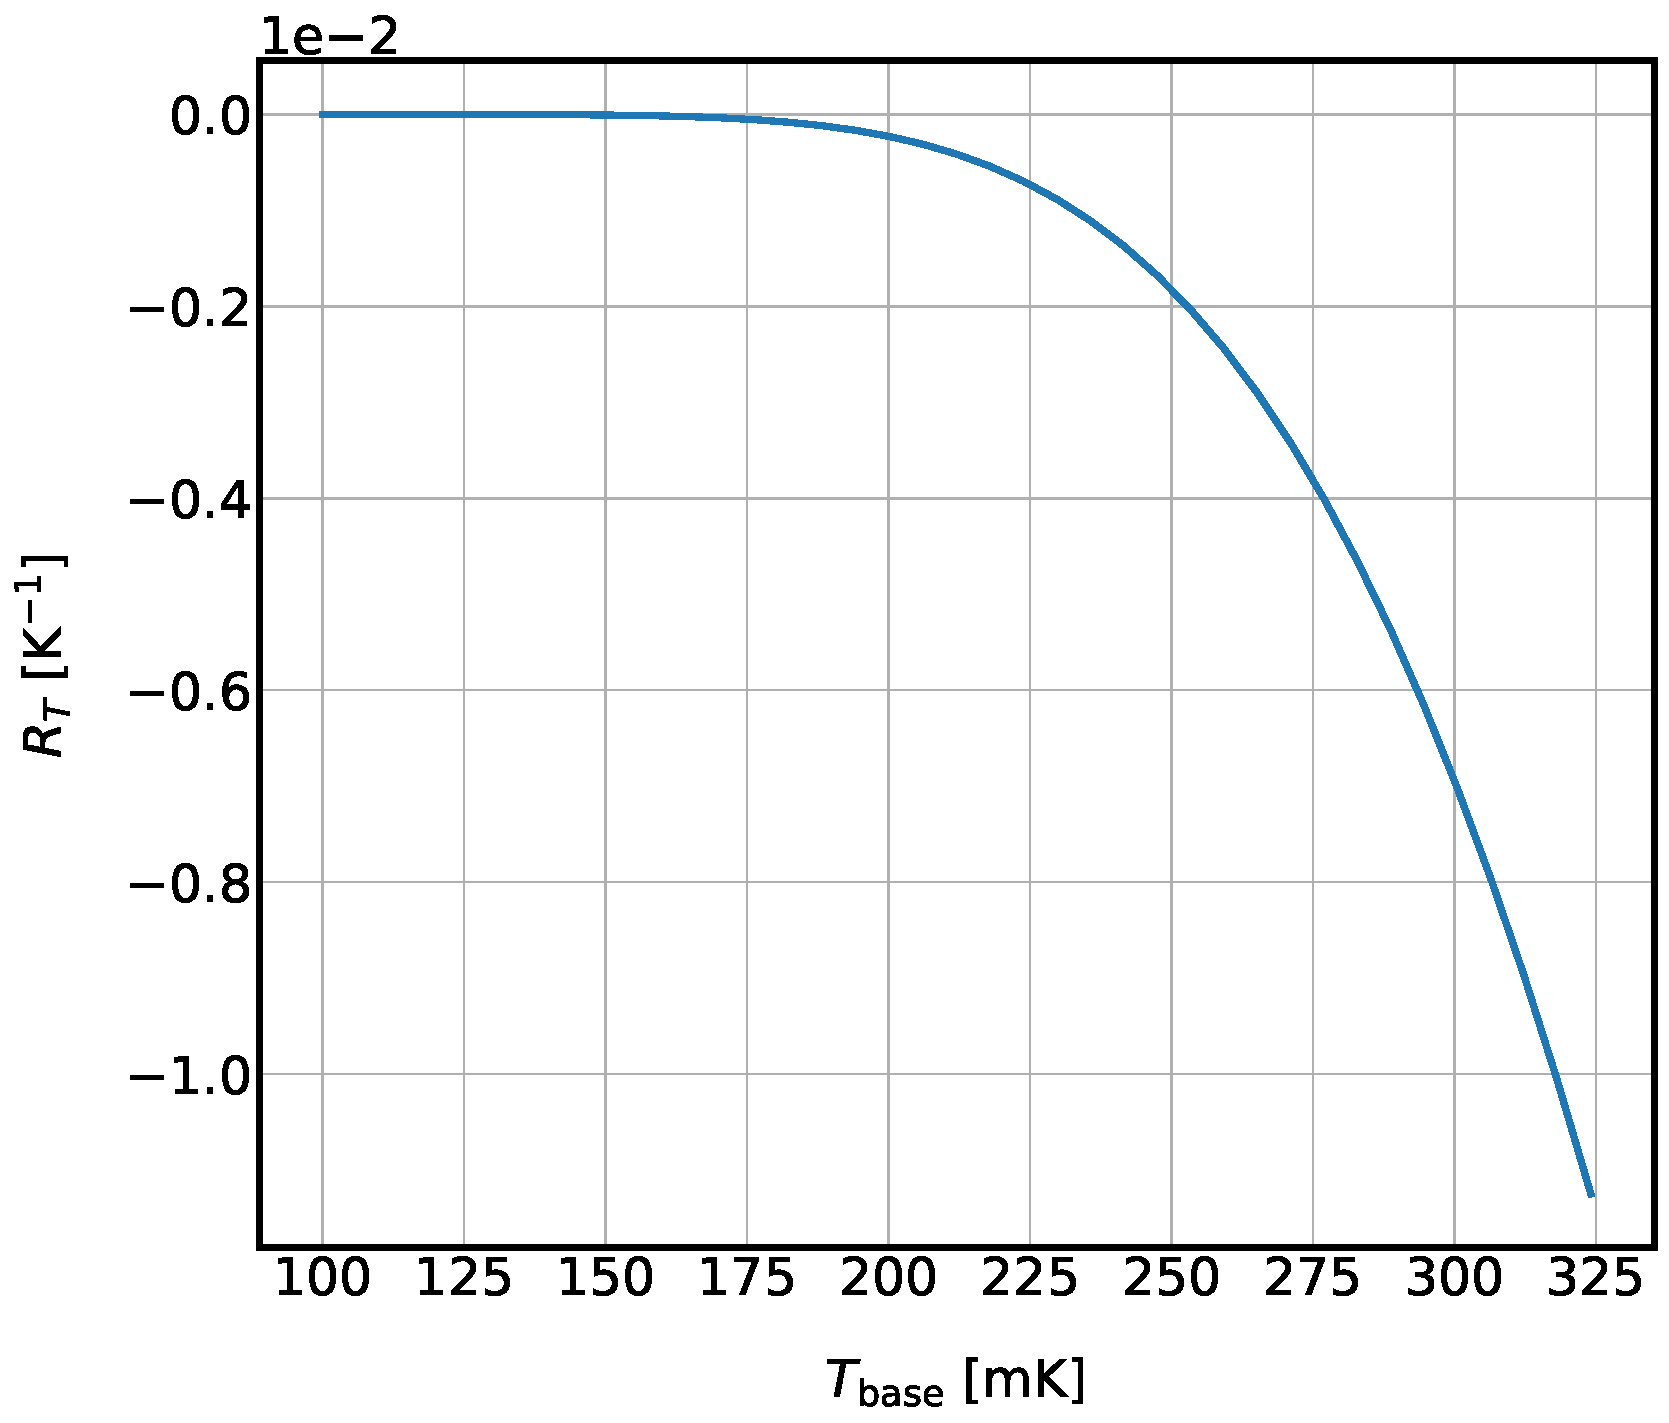
\includegraphics[width=\textwidth]{figures/kid_model/dfdT}
\caption[~Simulated LEKID temperature responsivity.]{Simulated LEKID temperature responsivity \gls{Rtemp}.}
\label{fig:dfdT}
\end{figure}

\subsection{Optical Responsivity}

At a fixed base temperature, the change in the LEKID's resonant frequency in response to a change in absorbed optical power can be written as:

\begin{equation}
    R_{P} = \frac{df_{0}}{d\gls{Pabs}} = \frac{df_{0}}{d\gls{sig2}} \frac{d\gls{sig2}}{d\gls{nqp}} \frac{d\gls{nqp}}{d\gls{Pabs}}
\end{equation}

where:

\begin{equation}
  \frac{df_{0}}{d\gls{sig2}}\frac{d\gls{sig2}}{d\gls{nqp}} \simeq -\frac{\alpha f_{0}} {4\gls{N0}\gls{Delta}} \left( 1 + \sqrt{ \frac{2 \Delta_{0}}{\pi K T}} \right)
\end{equation}

The expression for $\frac{d\gls{nqp}}{d\gls{Pabs}}$ is case dependent. Here, we provide a brief overview of three cases, as found in \citet{mauskopf2018transition}. We first consider the rate of change in the total number density of QP\@:

\begin{equation}\label{eq:dn_dt}
  \begin{aligned}
  \frac{\gls{nqp}}{dt} &= \Gamma_{opt} + \Gamma_{ro} + \Gamma_{therm} + \Gamma_{rec} \\
   &= \frac{\gls{det_eff} \gls{Pabs}}{\Delta \Sigma} + \frac{\epsilon_{ro} P_{ro}}{\Delta \Sigma} + \gamma \gls{N0}^{2} 8\pi k T \Delta e^{-2 \Delta / kT} -\frac{\gls{nqp}}{\gls{tau_qp}}
  \end{aligned}
\end{equation}

where:
\begin{itemize}[label={},nosep]
  \item $\Gamma_{opt}$ is the QP generation rate due to absorbed optical power.
  \item $\Gamma_{ro}$ is the QP generation rate due to microwave readout power.
  \item $\Gamma_{therm}$ is the QP generation rate due to thermal phonons.
  \item $\Gamma_{rec}$ is the QP recombination rate into CPs.
  \item \gls{det_eff} is the efficiency of QP generation from absorbed optical power.
  \item $\epsilon_{ro}$ is the internal QP generation efficiency for absorbed readout power.
  \item $\gamma = 1/(\gls{nqp}\gls{tau_qp})$ is a constant relating the number density of QP to the QP recombination time.
\end{itemize}

In the first case (\textit{Case 1}), we assume that QP generation is dominated by the absorption of photons. Equation~\ref{eq:dn_dt} then becomes

% case 1

\begin{equation}
    \frac{\gls{nqp}}{dt} \simeq \frac{\gls{det_eff} \gls{Pabs}}{\Delta \Sigma} - \gamma\gls{nqp}^{2}
\end{equation}

Then, $\frac{d\gls{nqp}}{dP\gls{Pabs}}$ can be shown to be:

\begin{equation}\label{eq:case1}
  \frac{d\gls{nqp}}{d\gls{Pabs}} = \frac{1}{2}\sqrt\frac{\eta}{\gamma \gls{Pabs}\Delta\Sigma} = \frac{n_{0}}{2\gls{Pabs}} \frac{1}{1 + j\omega\gls{tau_qp}/2}
\end{equation}

Behavior corresponding to \textit{Case 1} has been observed in Al KIDs (e.g., \citet{de2014quasiparticle,flanigan2016photon,mauskopf2014photon}).

The second case to consider \textit{Case 2} is if the QP generation rate is dominated by thermal phonon generation, or has a recombination time that does not depend on \gls{Pabs}. In this case, Equation~\ref{eq:dn_dt} becomes:
% case 2

\begin{equation}
    \frac{\gls{nqp}}{dt} \simeq \frac{\gls{det_eff} \gls{Pabs}}{\Delta \Sigma} + \Gamma_{therm} - \frac{\gls{nqp}}{\tau_{\mathrm{eff}}}
\end{equation}

and

\begin{equation}\label{eq:case2}
\frac{d\gls{nqp}}{d\gls{Pabs}} \simeq \frac{\eta\tau_{\mathrm{eff}}}{\Delta\Sigma}\frac{1}{1 + j\omega\tau_{\mathrm{eff}}}
\end{equation}

Behavior corresponding to \textit{Case 2} has been observed in TiN KIDs (e.g., \citet{catalano2014performance,hubmayr2015photon,hailey2016low}).

% intermediate case
In the intermediate case, there is an effective `dark' power loading on the device, $P_{\mathrm{dark}}$, which generates a constant background of QP whose rate of creation is independent of absorbed optical power. In this case,

\begin{equation}
    \frac{\epsilon_{ro} P_{ro}}{\Delta \Sigma} + \gamma \gls{N0}^{2} 8\pi k T \Delta e^{-2 \Delta / kT} - \gamma\gls{nqp}^{2}
\end{equation}

and

\begin{equation}
  \frac{d\gls{nqp}}{dP_{\mathrm{abs}}} = \sqrt{\frac{\gls{det_eff}}{\Delta \Sigma \gamma}}\frac{1}{\sqrt{P_{\mathrm{dark}} + \gls{Pabs}}}
\end{equation}

\begin{figure}[!htbp]
\centering
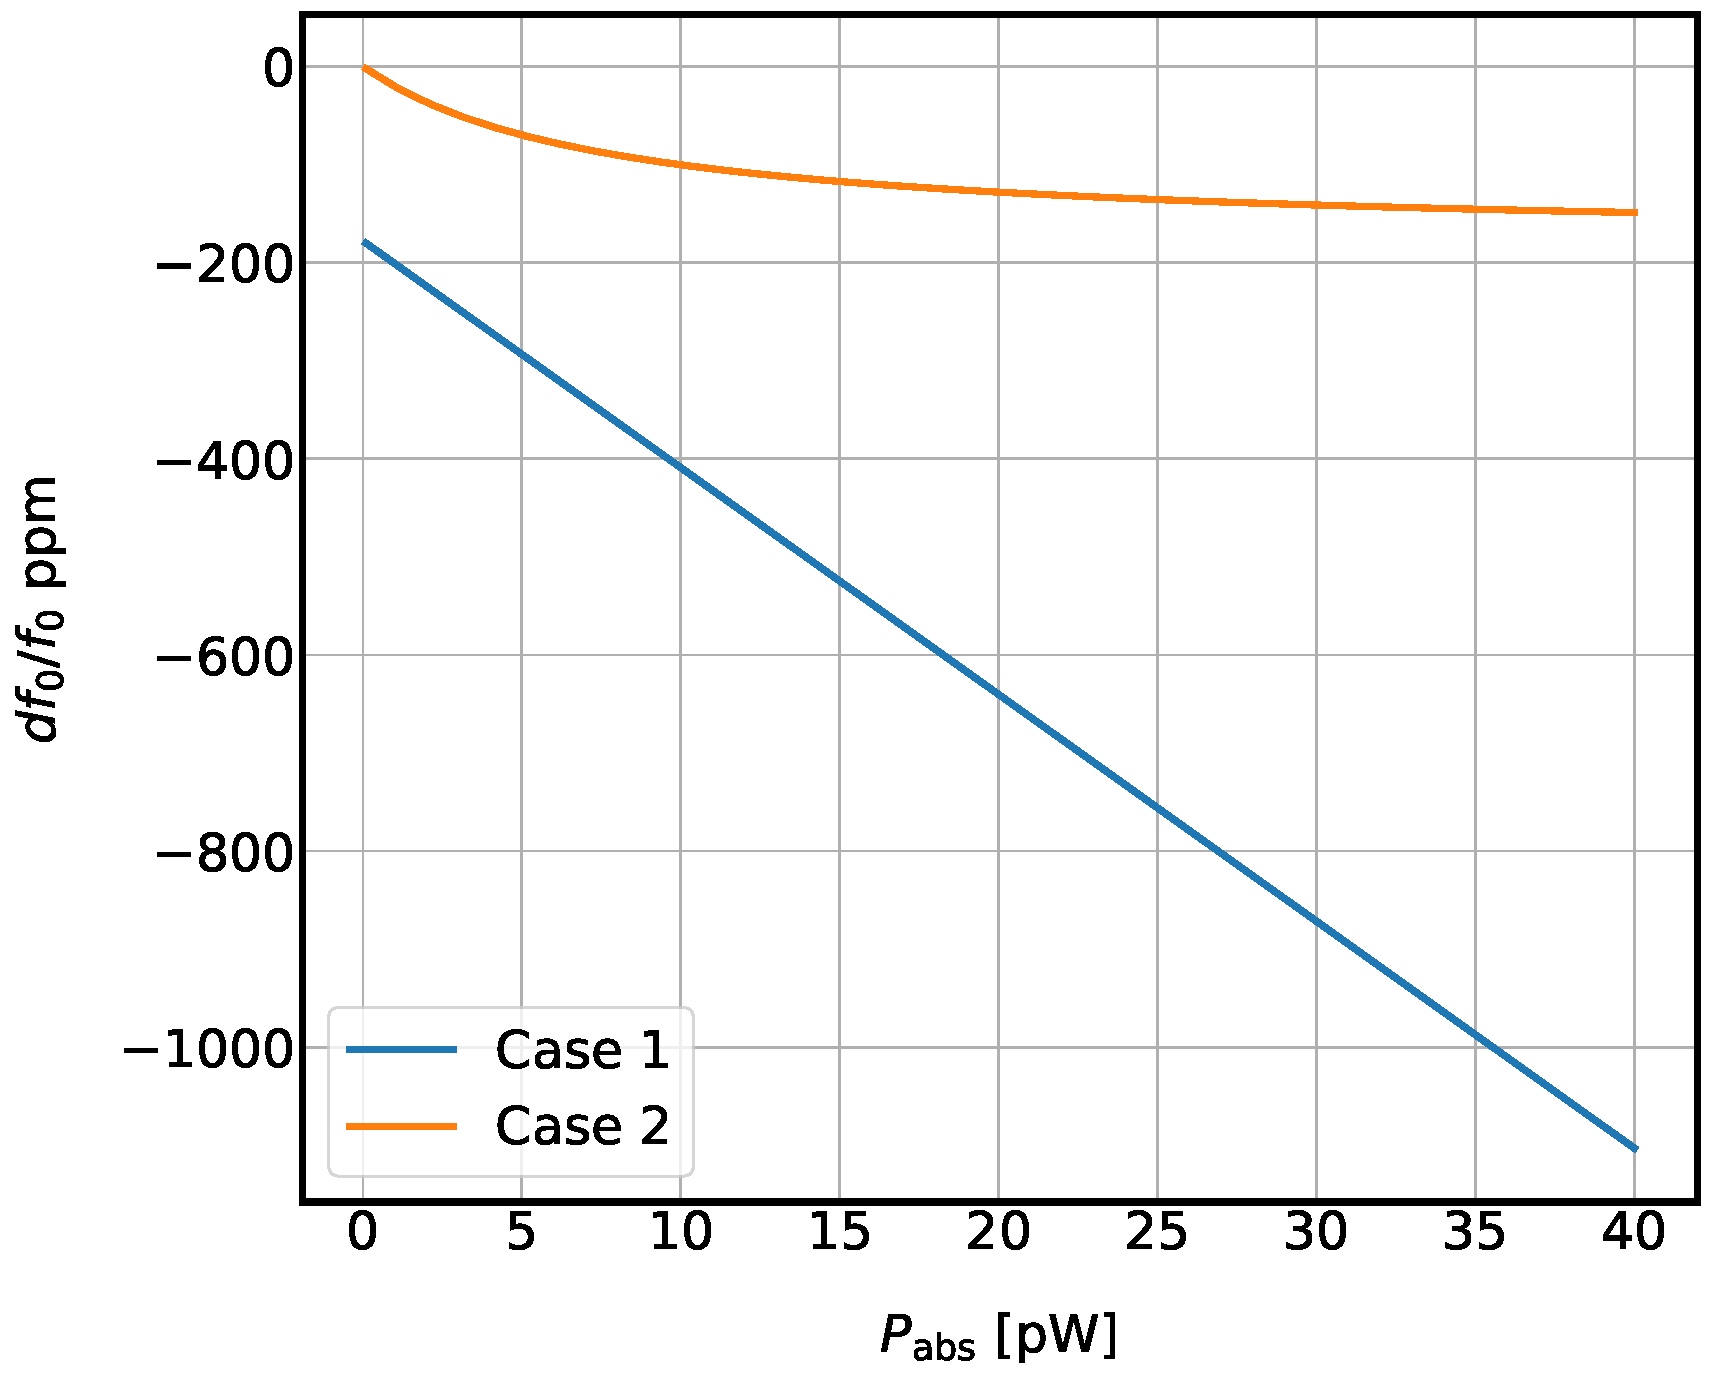
\includegraphics[width=\textwidth]{figures/kid_model/resp_case1_case2}
\caption[~A model of the case~1 and case~2 optical responsivities.]{A model of the \textit{Case 1} and \textit{Case 2} optical responsivities.}
\label{fig:responsivity}
\end{figure}

\begin{figure}[!htbp]
\centering
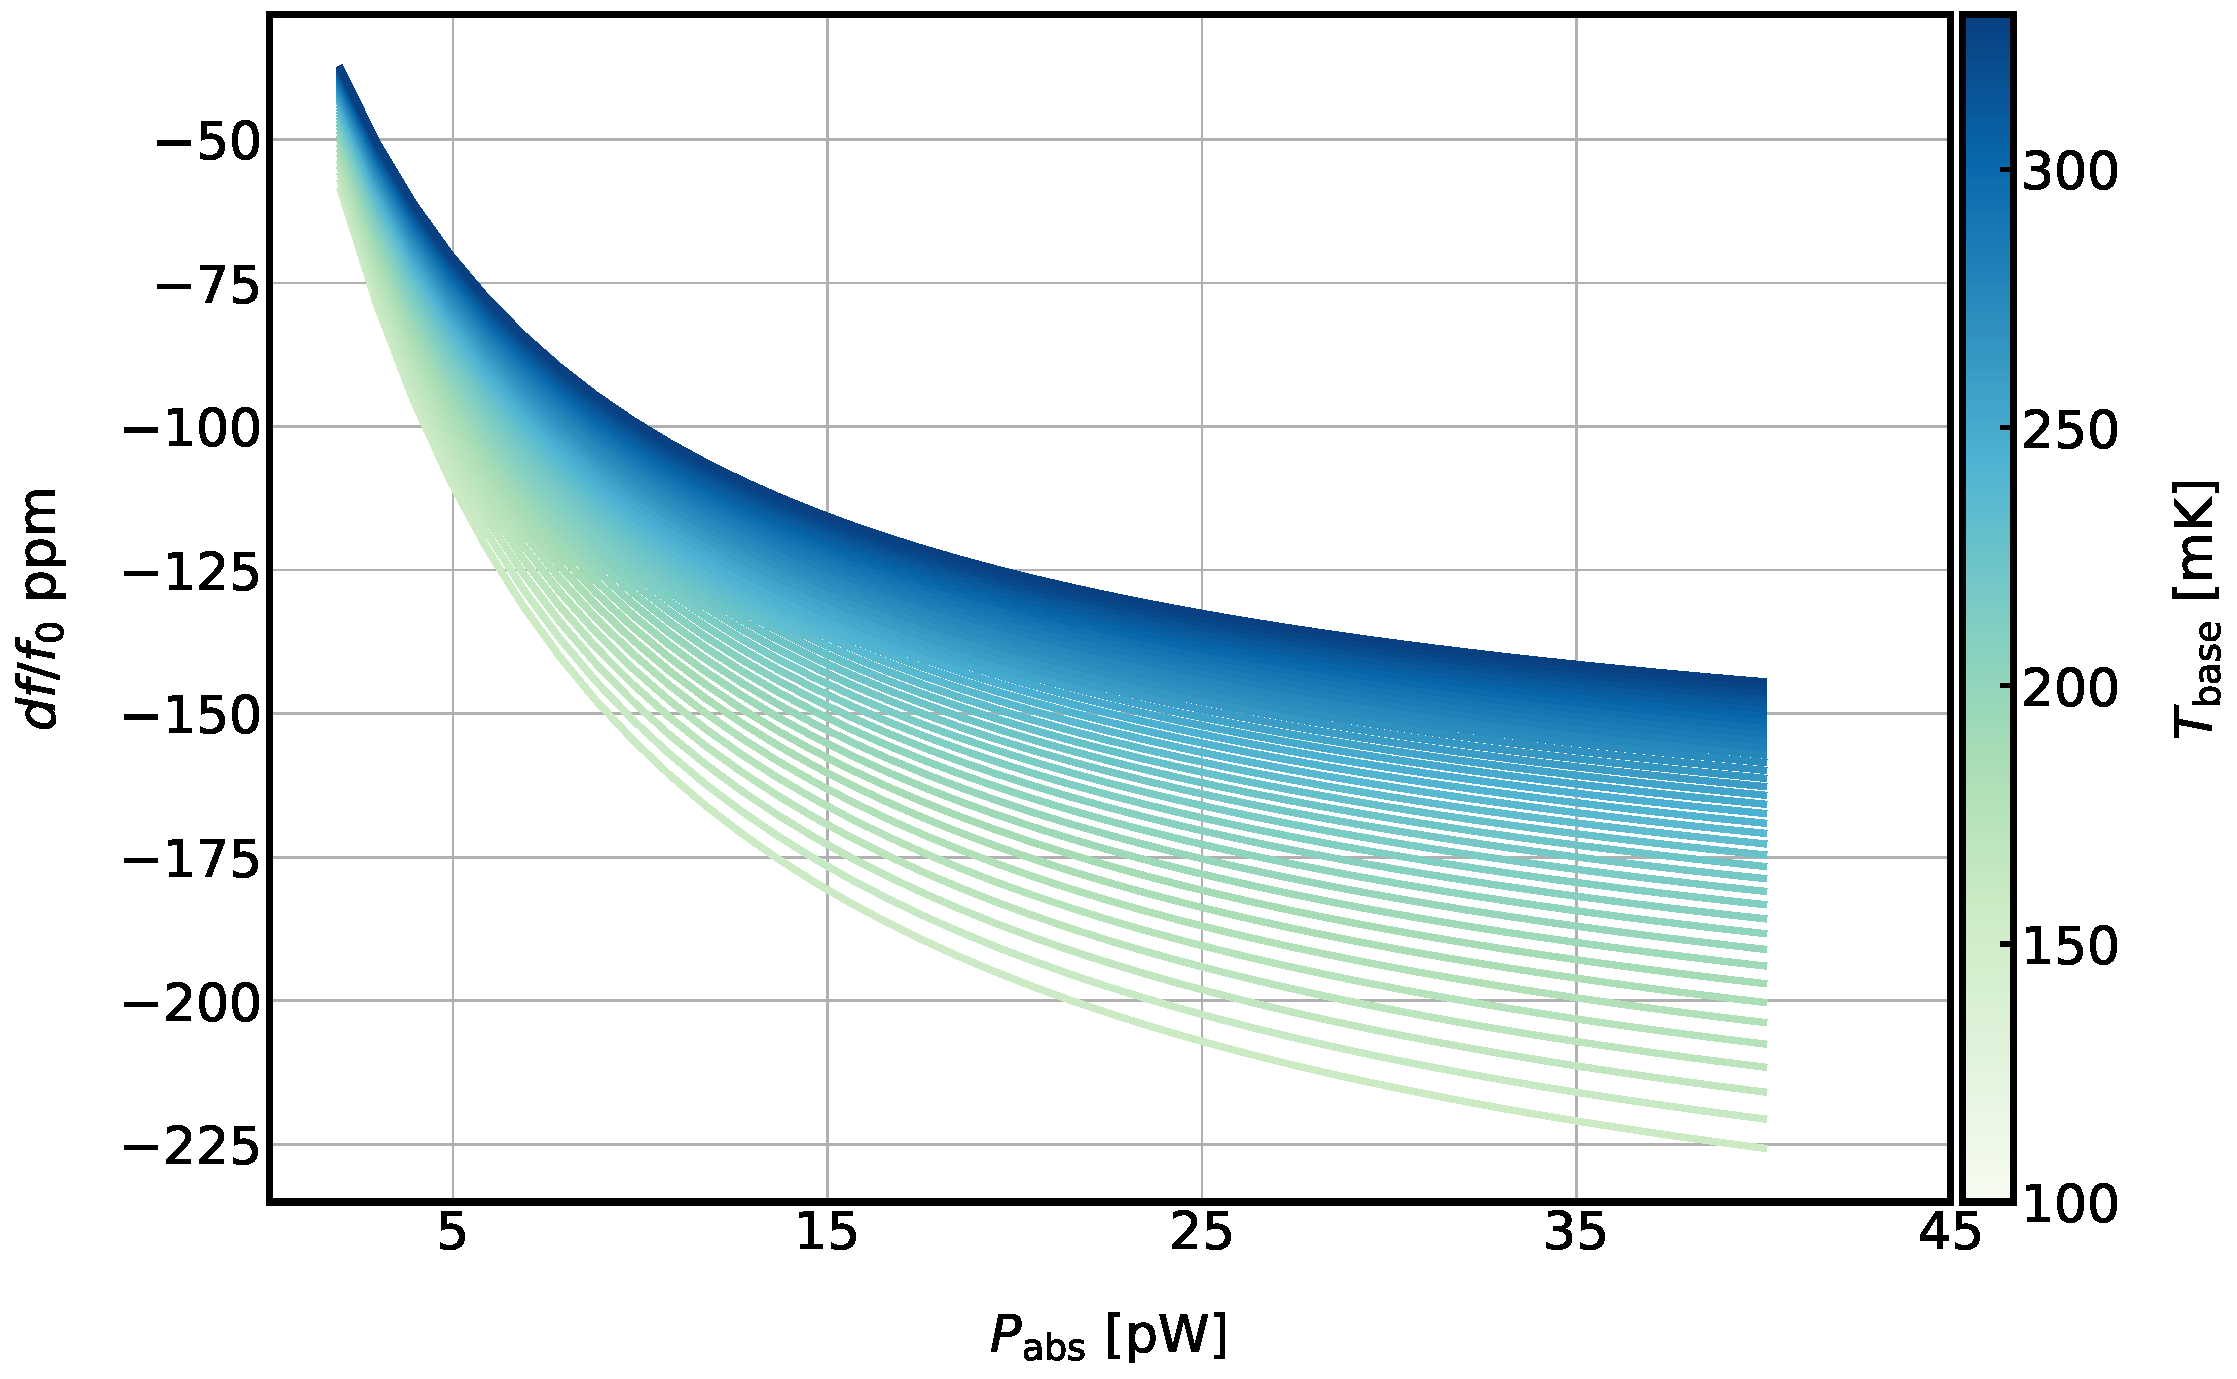
\includegraphics[width=\textwidth]{figures/kid_model/resp_case2_T}
\caption[~The case~2 responsivity shown for a range of base temperatures.]{The \textit{Case 2} responsivity shown for a range of base temperatures.}
\label{fig:case 2 responsivity}
\end{figure}

A model of the \textit{Case 1} and \textit{Case 2} responsivities is shown in Figure~\ref{fig:responsivity}. In \textit{Case 1}, the frequency shift due to absorbed power, in fractional frequency units ($df_{0}/f_{0}$) is linear. In \textit{Case 2}, the frequency shift is approximately linear for low amounts of absorbed power, then asymptotically approaches a constant value at higher powers. Figure~\ref{fig:case 2 responsivity} shows the \textit{Case 2} responsivity for a range of base temperatures. The slope of the low-power, linear part of the curve becomes steeper at lower \gls{Tbase}.

\subsection{The Nonlinear Kinetic Inductance}\label{nonlinearKI}

The KI has a second-order term whose effects on various LEKID parameters must be considered during the biasing stage of detector calibration. The nonlinear KI can be written as a function of internal current, $I_{\mathrm{int}}$:

% Nonlinear KI
\begin{equation} \label{eq:nonlinear KI}
  \gls{Lk_per_l}(I_{\mathrm{int}}) = \gls{Lk_per_l}(0) \left[ 1 + \left( \frac{I_{\mathrm{int}}}{I_{\star}} \right) \right]
\end{equation}

where $I_{\star}$ is the critical current corresponding to the maximum charge-carrier velocity before pair-breaking occurs (\citet{tinkham2004introduction,anlage1989current,annunziata2010tunable}). In a LEKID camera, the source of this internal current is the microwave probe tone generated by the readout system. For LEKIDs, the readout tone power, $P_{ro}$, at the device typically ranges from $\sim$-60 to -120 dBm.
The nonlinearity adds an additional frequency detuning $\delta x$, of $\mathcal{O}(I^{2}/I_{\star}^{2})$:

\begin{equation}
  \delta x = \frac{\delta \omega}{\omega_{0}} = -\frac{1\delta L}{2L} = \frac{\alpha}{2}\left( \frac{I}{I_{\star}} \right)^{2} = -\frac{E_{r}}{E_{\star}}
\end{equation}

where $E_{r}$ is the internal resonator energy, and $E_{\star} = LI_{\star}^{2}/2\alpha = \gls{N0} \Delta^{2} \Sigma/2$ is the condensation energy of the inductor (\citet{mauskopf2018transition,tinkham2004introduction}). As in Section~\ref{sec:kinetic_inductance}, the resonator current is related to the internal resonator energy by the inductance (here assuming that $L_{m} \ll L_{K}$). The resonator energy can be written as a function of tone power \citep{swenson2013operation}, as:

% Resonator energy
\begin{equation}
 \begin{aligned}
  E_{r} &= \frac{1}{2}LI_{\mathrm{int}}^{2}\\
        &= \frac{2\gls{Qr}^{2}}{\gls{Qc}}\frac{1}{1 + 4\gls{Qr}^{2}x^{2}}\frac{P_{ro}}{\omega_{r}}
  \end{aligned}
\end{equation}

where $\omega_{r}$ is the shifted resonant frequency.

The total fractional detuning, $x$, is an implicit equation:

\begin{equation} \label{eq:implicit detuning}
  \begin{aligned}
  x &= x_{0} + \delta x \\
    &= x_{0} -\frac{E_{r}(x)}{E_{\star}}
    \end{aligned}
\end{equation}

Using the relations above, it's possible to estimate the degree of nonlinearity from a frequency sweep of  \gls{S21}. In standard practice, it's preferable to bias each resonator so that the frequency detuning contributed by the readout tone power is less than one resonator line-width (FWHM). This ensures that the resonator doesn't bifurcate. The width of the resonator is $\delta \omega \simeq \omega_{0}/\gls{Qr}$. Therefore, the fractional detuning due to the nonlinearity should be: $\left| \delta x \right| = \frac{E_{r}}{E_{\star}} < \frac{1}{\gls{Qr}}$. Using the equations above, satisfying this condition requires that an upper limit to the internal resonator energy is:

% maxmimum resonator energy before bifurcation
\begin{equation}
  E_{r} < \frac{\gls{N0}\gls{Delta}^{2}\Sigma}{2\gls{Qr}}
\end{equation}

and the maximum readout tone power is:

% maximum readout power before nonlinearity
\begin{equation} \label{eq:Pmax}
  P_{ro} < \frac{\gls{Qc}}{2\gls{Qr}^{3}}\gls{N0}\Delta^{3}\Sigma\omega\left(1 + 4\gls{Qr}^{2}x^{2} \right)
\end{equation}

At a fixed base temperature, larger optical loading permits the use of higher probe tone powers. This behavior is illustratd in Figure~\ref{fig:Pmax}, which shows the maximum probe tone power for a range of optical powers.

\begin{figure}[!htbp]
\centering
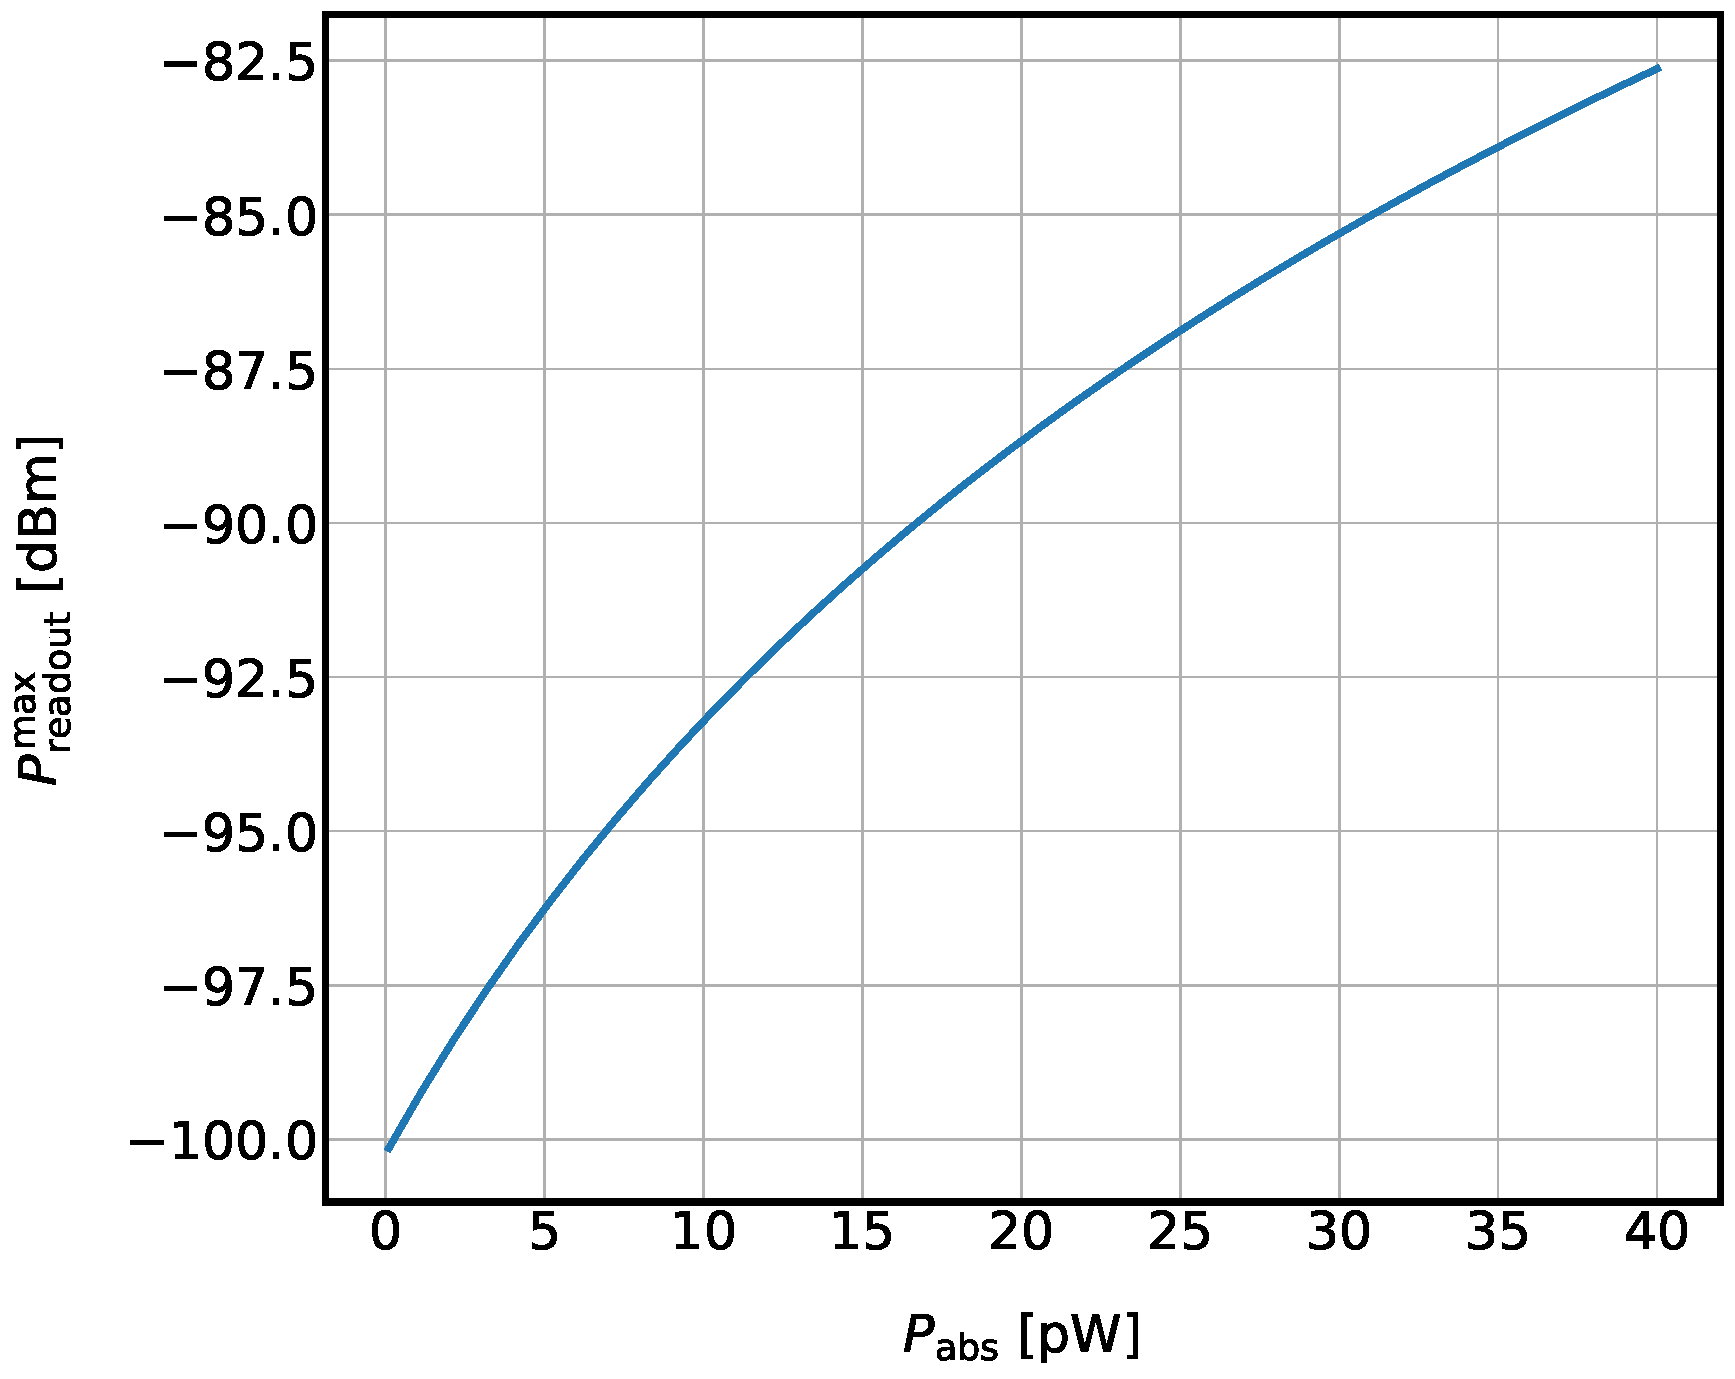
\includegraphics[width=\textwidth]{figures/kid_model/Pmax}
\caption[~The maximum probe tone power shown for a range of optical power loadings.]{The maximum probe tone power shown for a range of optical power loadings.}
\label{fig:Pmax}
\end{figure}

\subsection{Bifurcation}\label{bifurc}

At a particular probe tone power, the resonance enters an unstable equilibrium between two states, which is known as bifurcation. This phenomenon can be understood from the perspective of soft-spring Duffing effects (see, e.g., \citet{swenson2013operation,duffing1918erzwungene}). Bifurcation can be induced during an \gls{S21} frequency sweep, by sweeping the resonance either from below or from above the resonant frequency. These two cases correspond to positive and negative feedback, respectively.

\textit{Upward sweep, positive feedback}:
As the probe tone is swept upward in frequency from below the resonant frequency, the resonant frequency is detuned, and drawn toward the probe tone frequency. This positive feedback increases until the resonator bifurcates between the energized state and its rest state.

\textit{Downward sweep, negative feedback}:
As the probe tone is swept downward in frequency from below the resonant frequency, the resonator is detuned farther below the probe tone frequency. When the probe tone eventually passes the resonant frequency, the resonator bifurcates between its energized and rest states.

The bifurcation power can be estimated using Equation~\ref{eq:Pmax}. If the resonator quality factor is dominated by the coupling quality factor, $\gls{Qr} \approx \gls{Qc}$, and $x \ll 1$,

% bifurcation power
\begin{equation} \label{eq:Pbifurc}
  P_{\mathrm{bifurc}} = \frac{1}{2 \gls{Qc}^{2}}\gls{N0}\Sigma \omega_{0}\Delta^{2}
\end{equation}

\section{Sensitivity}\label{sec:sensitivity}

The sensitivity of a sub-mm detector is typically reported as either a noise-equivalent power (NEP) or noise-equivalent temperature (NET). The NEP (NET) describes the detector's sensitivity to absorbed optical power (temperature). NEP is commonly written in units of $\mathrm{W}/\sqrt{\mathrm{Hz}}$. This represents the noise power inside a measurement bandwidth of 1~Hz. Equivalently, it is the noise power which is measured after a 0.5~second integration (by the Shannon-Nyquist sampling theorem). At the time of writing, typical KID NEPs (under optical loading) are of $\mathcal{O}(10^{-17})$~$\mathrm{W}/\sqrt{\mathrm{Hz}}$. With that NEP, one can measure a signal level of $10^{-17}$~W with a signal-to-noise-ratio (SNR) of 1, over a 0.5~s integration.

KIDs, like most other astronomical detectors, are designed to be photon noise limited. Photon noise follows Poisson, or shot noise statistics. In a measurement dominated by shot noise, the SNR increases as $\sqrt{N}$, where $N$ is the number of measurements. In a typical sub-mm observation, the detector noise is limited by the shot noise of the background of in-band photons emanating from the receiver, optical system, atmosphere and astronomical source. In this scenario, the detectors are said to be operating in the background-limited IR photodetector (BLIP) limit.

During an on-sky KID measurement, it is preferable to view the detector timestreams in units of frequency shift (or fractional frequency) \gls{df}, relative to the resonant frequency of each pixel. If a responsivity (e.g., $df/dT$, $df/dP$) is known, then the NEP (or NET) can be calculated by dividing the square-root of the power spectral density (PSD) of the frequency fluctuations (units of Hz/$\sqrt{\mathrm{Hz}}$) by the corresponding responsivity.

\subsection{Instrumental Noise Hierarchy}

The NEP which is calculated during a measurement is the sum of contributions from several different noise sources. The order in which each noise source should dominant forms the instrumental noise hierarchy. In a LEKID camera, the noise hierarchy (from most to least dominant) is:

\begin{itemize}[nosep]
  \item Photon noise
  \item Amplifier noise (dominated by the first-stage cryogenic low noise amplifier (LNA))
  \item Detector noise (generation-recombination (GR))
  \item Readout noise
\end{itemize}

The readout noise is discussed in Chapter~\ref{readout}. The other three noise sources are treated individually in the following sections.

\subsection{Generation-Recombination Noise}\label{ssec:GR noise}

In the absence of readout and amplifier noise, the intrinsic noise floor of a KID measurement is set by GR noise. GR noise originates from the instantaneous uncertainty in the rate of CPs recombining into QPs (or, equivalently, the rate at which CPs are broken into QP pairs). A simple expression for the GR contribution to the fractional noise spectral density follows from a consideration of the generation and recombination rates (\gls{gen_rate} and \gls{rec_rate}), assuming a steady state ($\gls{gen_rate} = \gls{rec_rate}$). The uncertainty in the number of CPs is:

\begin{equation}\label{eq:dNcp1}
  \begin{aligned}
  \delta N_{cp} &= \gls{gen_rate}\delta t - \gls{rec_rate}\delta t \\
                &= \sqrt{(\gls{gen_rate} + \gls{rec_rate})\delta t} \\
                &= \sqrt{2\gls{rec_rate}\delta t}
  \end{aligned}
\end{equation}

where $\delta t = 1/2 \delta f$ is the measurement integration time (with measurement bandwidth $\delta f$). Using the fact that $\gls{rec_rate} = \frac{\gls{Nqp}}{2\gls{tau_qp}}$, the uncertainty in the recombination rate is:

\begin{equation}
  \begin{aligned}
  \delta \gls{rec_rate} &= \frac{\delta N_{cp}}{\delta t} \\
                        &= \sqrt{ \frac{2\gls{rec_rate}}{\delta t}} \\
                        &= \sqrt{ \frac{2\gls{Nqp}}{2\gls{tau_qp}\delta t} }
  \end{aligned}
\end{equation}

Equation~\ref{eq:dNcp1} becomes:

\begin{equation}\label{eq:dNcp2}
  \begin{aligned}
  \delta N_{cp} &= \delta \gls{rec_rate} \gls{tau_qp} \\
                &= \sqrt{ \frac{\gls{Nqp} \gls{tau_qp}}{\delta t} } \\
                &= \sqrt{2\gls{Nqp}\gls{tau_qp} \delta f}
  \end{aligned}
\end{equation}

Dividing Equation~\ref{eq:dNcp2} by the square-root of the measurement bandwidth, and multiplying by the frequency responsivity to fluctuations in the number of QP yields an expression for the frequency noise PSD\@:

\begin{equation} \label{eq:ef GR}
e_{f,GR} = \sqrt{2 \gls{Nqp}_{\mathrm{,tot}}\gls{tau_qp}}\frac{df_{0}}{d\gls{Nqp}}
\qquad \left[ \frac{\mathrm{Hz}}{\sqrt{\mathrm{Hz}}} \right]
\end{equation}

From Equation~\ref{eq:ef GR}, the NEP contribution from GR can be calculated as:

\begin{equation} \label{eq:NEP GR}
  NEP_{GR} = e_{f,GR} \bigg/ \left( \frac{df_{0}}{d\gls{Nqp}}\frac{d\gls{Nqp}}{d\gls{Popt}} \right) \qquad \left[ \frac{\mathrm{W}}{\sqrt{\mathrm{Hz}}} \right]
\end{equation}

\subsection{Two-Level System Noise}\label{ssec:TLS}

Nonthermal two-level system (TLS) fluctuations occur throughout the amorphous dielectric layer of the superconducting substrate. The TLS systems have electric and magnetic dipoles which can interact with external fields around the device. These interactions manifest as fluctuations in the complex permittivity and/or permeability of the material. In a KID, random fluctuations in $C_{r}$ are indistinguishable from fluctuations in KI, because both introduce jitter to the resonant frequency. The TLS noise is generally modeled as being capacitive in origin (see, e.g., \citet{gao2008physics,zmuidzinas2012superconducting}). It is thought to be the underlying cause of an often observed anomalous increase in resonant frequency with increasing base temperature (a violation of predictions made by MB theory), however other explanations have been offered (see, e.g., the Kondo effect \citep{noguchi2018analysis}).

The TLS loss tangent, $\delta_{TLS}$, can limit the \gls{Qi} of a KID, and has an empirical dependence on the internal power stored in the resonator (proportional to microwave probe tone power), expressed as (\citet{barry2014development,martinis2005decoherence}):

\begin{equation}
  \delta_{TLS} = \gls{Qi}^{-1} = F_{TLS}\delta_{0} \left(\frac{1}{1 + \left| P_{\mathrm{int}}/P_{c} \right|} \right)^{1/2}
\end{equation}

where:
\begin{itemize}[label={},nosep]
  \item $F_{TLS}$ is the ratio of the electric field stored in the TLS systems to the total electric field
  \item $\delta_{0}$ is the intrinsic loss tangent
  \item $\chi = \hbar\omega/2kT$
  \item $P_{\mathrm{int}}$ is the internal resonator microwave power
  \item $P_{\mathrm{sat}}$ is the TLS saturation power
\end{itemize}

where $\delta_{TLS}$ is known to saturate above a characteristic power, $P_{\mathrm{sat}}$. Because the maximum microwave readout power which can be used before nonlinearity sets in (Equation~\ref{eq:Pmax}) is proportional to inductor volume ($P_{ro\mathrm{,max}} \propto \Sigma$). The TLS noise therefore increases as $\Sigma^{1/2}$. The number of TLS systems scales with the volume of the amorphous dielectric, or $\Sigma$, and the way in which the KID responsivity varies with $\Sigma$ depends on the substrate material (see Section~\ref{sec:responsivity}).

For Al KIDs, the responsivity does not depend on $\Sigma$ (Equation~\ref{eq:case1}). The TLS noise therefore increases relative to GR and other noise sources as $\Sigma^{1/2}$, and the inductor volume can be made large. In TiN KIDs, $df_{0}/d\gls{Pabs} \propto \Sigma^{-1}$, and these devices typically use smaller $\Sigma$ \citep{mauskopf2018transition}. TLS noise mitigation techniques which involve the use of crystalline, rather than amorphous dielectrics, are presently an active area of research (see, e.g., \citet{weber2011single}).

A semi-empirical model for the TLS noise spectral density is presented in \citet{gao2008semiempirical}. The noise PSD has a colored spectrum ($\gls{Sxx} \propto f^{-\alpha}$) with spectral index $\alpha \approx 0.5$, and depends on microwave readout power and \gls{Tbase} as:

\begin{equation}\label{eq:Sx_TLS}
  \gls{Sxx}_{,TLS} \propto T^{-t}P_{ro}
\end{equation}

where $t =$ 1.5--2. $NEP_{TLS}$ can be found by dividing Equation~\ref{eq:Sx_TLS} by a responsivity (e.g., \gls{Rtemp} or \gls{Ropt}).

\subsection{Amplifier Noise}\label{ssec:amp noise}

The LNA which is used to amplify the probe tone comb at the output of the KID array adds thermal, or Johnson-Nyquist noise to the signal (\citet{johnson,nyquist1928thermal}). Johnson-Nyquist noise in a resistor originates from thermal motions of the electrons which manifest as voltage fluctuations across its terminals. Following \citet{kittel1998thermal}, an expression for the RMS voltage contribution from Johnson-Nyquist noise is found by considering a simple circuit model. The circuit consists of a white noise generator with resistance $R$ which transfers power to a resistive load with resistance $R_{L}$. The power transferred from the noise generator to the load is:

\begin{equation}
  P = \left<I^{2}\right>R_{L} = \frac{\left<V^{2}\right>R}{(R + R_{L})^{2}}
\end{equation}

The maximum power transfer occurs when the source and load are perfectly matched ($R = R_{L}$). In this case,

\begin{equation}
 P = \frac{\left<V^{2}\right>R}{4R}
\end{equation}

and the RMS voltage is:

\begin{equation}
  \left<V^{2}\right> = 4PR = 4kT\int_{f_{0}}^{f_{1}} R df = 4kTRB
\end{equation}

where $T$ is the temperature of the Thevenin equivalent of the circuit, and $B$ is the bandwidth over which the voltage is being measured. The resistance is assumed to be constant with frequency. Returning to the case of the LNA, the one-sided PSD of the voltage fluctuations is:

\begin{equation} \label{eq: johnson noise}
   e_{V,\mathrm{amp}} = 4kT_{\mathrm{amp}}Z \qquad  \left[ \frac{\mathrm{V}^{2}}{\mathrm{Hz}} \right]
\end{equation}

where $Z = R$ is the input impedance of the amplifier. The PSD is converted to frequency units by dividing by the voltage responsivity:

\begin{equation} \label{eq:ef amp}
  \begin{aligned}
  e_{f,\mathrm{amp}}^{2} &= \frac{e_{v,\mathrm{amp}}^{2}}{\left| dV/df_{0} \right|^{2}} \\
  \end{aligned}
\end{equation}

The voltage responsivity can be approximated using Equation~\ref{eq:S21}:

\begin{equation}
  \begin{aligned}
  \frac{dV_{\mathrm{out}}}{df_{0}} &= V_{\mathrm{in}}\frac{d\gls{S21}}{df_{\mathrm{out}}} \\
                         &\simeq -2jV_{\mathrm{in}}\frac{\gls{Qr}^{2}f_{\mathrm{probe}}}{\gls{Qc}f_{0}^{2}}\frac{1}{(1 + 2j\gls{Qr}x)^{2}}
  \end{aligned}
 \end{equation}

Near resonance, $x \ll 1$, and

\begin{equation}
  \frac{dV_{\mathrm{out}}}{df_{0}} \simeq 2jV_{\mathrm{in}}\frac{\gls{Qr}^{2}}{\gls{Qc}f_{0}}
\end{equation}

Equation~\ref{eq:ef amp} can then be written as:

\begin{equation}
  \begin{aligned}
  e_{f,\mathrm{amp}}^{2} &= 4kT_{\mathrm{amp}}Z_{0}\left( \frac{\gls{Qc}^{2}f_{0}^{2}}{4\gls{Qr}^{4}} \right) \\
               &= kT_{\mathrm{amp}}\left( \frac{\gls{Qc}^{2}f_{0}^{2}}{\gls{Qr}^{4}P_{ro}}\right) \\
               &= kT_{\mathrm{amp}}\left( \frac{f_{0}^{2}}{\gls{Qr}^{2}P_{ro}}\right)
  \end{aligned}
\end{equation}

where the probe tone power $P_{ro} = V_{\mathrm{in}}^{2}/Z_{0}$. For a resonator limited by the coupling quality factor ($\gls{Qr} \approx \gls{Qc}$),

\begin{equation}
  e_{f,\mathrm{amp}}^{2} = kT_{\mathrm{amp}}\left( \frac{f_{0}^{2}}{\gls{Qr}^{2}P_{ro}}\right) \qquad \left[ \frac{\mathrm{Hz}^{2}}{\mathrm{Hz}} \right]
\end{equation}

Therefore, for a probe tone near the resonant frequency, the frequency noise decreases with increasing readout power. As the tone power approaches the bifurcation power (Equation~\ref{eq:Pbifurc}), the frequency noise becomes independent of tone power. The LNA contribution to the NEP can therefore be written as:

\begin{equation}\label{eq:NEP amp}
  NEP_{\mathrm{amp}} = e_{f,\mathrm{amp}} \bigg/ \left( \frac{df_{0}}{d\gls{Nqp}}\frac{d\gls{Nqp}}{d\gls{Popt}} \right) \qquad \left[ \frac{\mathrm{W}}{\sqrt{\mathrm{Hz}}} \right]
\end{equation}

The $NEP_{\mathrm{amp}} \propto 1/\sqrt{P_{ro}} $ dependence makes it possible to suppress the amplifer noise contribution by using higher microwave readout powers.

\subsection{Photon Noise}\label{photon noise}

The optical power input into the system is assumed to be incoherent emission from a thermal blackbody source. To write an expression for the total optical power \gls{Popt}, we first consider the number of modes contained in the incident light beam, which has a central frequency $\nu$ and optical bandwidth $\Delta \nu$. The total number of modes is the product of the number of spatial, temporal and polarization modes:

\begin{equation}
 \begin{aligned}
  N_{\mathrm{modes}} &= \left( N_{\mathrm{spatial}} \right) \left( N_{\mathrm{temporal}} \right) \left( N_{\mathrm{pol}} \right) \\
            &= \left( \frac{A\Omega\nu^{2}}{c^{2}} \right) \left(\tau_{\mathrm{int}}\Delta \nu \right) \left(m\right)
  \end{aligned}
\end{equation}

where:
\begin{itemize}[label={},nosep]
  \item $A\Omega$ is the $\acute{e}$ntendue
  \item $\nu^{2}/c^{2} = \lambda^{2}$ is the $\acute{e}$ntendue of coherence
  \item $\tau_{\mathrm{int}}$ is the integration time
  \item $m$ is the number of polarization modes [1,2]
\end{itemize}

The photon arrival times follow Bose-Einstein statistics, with an occupation number, or mean number of photons per mode, of:

\begin{equation}
  \gls{n_occ} = \frac{\left< N_{\mathrm{photons}} \right> }{\mathrm{mode}} = \frac{1}{e^{h\nu/kT} - 1}
\end{equation}

where $T$ is the blackbody temperature of the source. With $m = 2$, the total optical power can be expressed as:

\begin{equation}\label{eq:P_opt}
 \begin{aligned}
  \gls{Popt} &= \left( N_{\mathrm{modes}} \times  \frac{\left< N_{\mathrm{phot}} \right>}{\mathrm{mode}} \times  \textrm{Energy per photon} \right) \bigg/ \tau_{\mathrm{int}} \\
          &= \left( \frac{m A\Omega\nu^{2}}{c^{2}} \right) \left(\tau_{\mathrm{int}}\Delta \nu \right)  \gls{n_occ} \frac{h\nu}{\tau_{\mathrm{int}}} \\
          &= A\Omega\Delta\nu \left( \frac{2h\nu^{3}}{c^{2}}\frac{1}{e^{h\nu/kT} - 1} \right) \\
          &= A\Omega\Delta\nu B_{\nu}(\nu, T) \qquad \left[ \mathrm{W} \right]
  \end{aligned}
\end{equation}

where $B_{\nu}(\nu, T)$ $\left[ \mathrm{W}\mathrm{m}^{-2}\mathrm{ str }^{-1}\mathrm{Hz}^{-1} \right]$ is the Planck function for spectral radiance. The incident power which is absorbed by the detectors is the total optical power multiplied by the optical efficiency \gls{opt_eff} and quantum efficiency of the detectors \gls{det_eff}:

\begin{equation}\label{eq:P_abs}
  \begin{aligned}
  \gls{Pabs} &= \gls{opt_eff}\gls{det_eff}\gls{Popt} \\
          &= \gls{opt_eff}\gls{det_eff} A\Omega\Delta\nu B_{\nu}(\nu, T) \qquad \left[ \mathrm{W} \right]
  \end{aligned}
\end{equation}

The mean-squared noise power measured by the detectors originates from fluctuations in \gls{n_occ}. Because its probability distribution function is the Bose-Einstein distribution, its variance is:

\begin{equation}
  \sigma^{2}_{n_{occ}} = \gls{n_occ} + \frac{ \gls{n_occ}^{2} }{N_{\mathrm{modes}}}
\end{equation}

where a factor corresponding to the case of $N_{\mathrm{modes}} \ll 1$ has been omitted (see, e.g., \citet{fox2006quantum,rowe2015passive}). The mean-squared noise power input to the optical system is therefore

\begin{equation}\label{eq:sigma_P}
  \begin{aligned}
  \sigma^{2}_{P} &= \sigma^{2}_{n_{occ}}N_{\mathrm{modes}}\left( \frac{h\nu}{\tau_{\mathrm{int}}} \right)^{2} \\
                 &= \frac{h\nu \gls{Popt}}{\tau_{\mathrm{int}}} + \frac{\gls{Popt}^{2}}{N_{\mathrm{modes}}} \qquad \left[ \mathrm{W}^{2} \right]
  \end{aligned}
\end{equation}

The noise spectral density (square-root of the NEP) is found by dividing Equation~\ref{eq:sigma_P} by the measurement bandwidth, $B = f_{s}/2 = \tau_{\mathrm{int}}$:

\begin{equation}\label{eq:Sxx_Popt}
  S_{xx} =  NEP_{\mathrm{phot}}^{2} = h\nu \gls{Popt} + \frac{\gls{Popt}^{2}}{N_{\mathrm{modes}}B} \qquad \left[ \frac{\mathrm{W}^{2}}{\mathrm{Hz}} \right]
\end{equation}

When the NEP is expressed in terms of \gls{Popt}, it is referred to as the \textit{electrical} NEP\@. When the NEP is expressed in terms of \gls{Pabs}, it is referred to as the \textit{optical} NEP\@. The first term in Equation~\ref{eq:Sxx_Popt} dominates for low \gls{n_occ} (shot noise limit, $h\nu / kT \gg 1$), and the second term dominates for high occupation number (wave noise limit, $h\nu / kT \ll 1$):

\begin{equation}\label{eq:NEP phot}
NEP_{\mathrm{phot}}^{2} = NEP_{\mathrm{shot}}^{2} + NEP_{\mathrm{wave}}^{2} \\
\end{equation}

In each of BLAST-TNG's three observation bands (250, 350 and 500~$\upmu$m) the shot noise term dominates the NEP\@. In frequency units, the NEP can be calculated as:

\begin{equation} \label{eq:ef phot}
  e_{f,\mathrm{phot}} = NEP_{\mathrm{phot}}\frac{df_{0}}{dN_{qp}}\frac{dN_{qp}}{d\gls{Popt}} \qquad \left[ \frac{\mathrm{Hz}}{\sqrt{\mathrm{Hz}}} \right]
\end{equation}

\subsection{Total NEP}

In frequency units, the total noise spectral density measured by the detectors is the quadrature sum of the noise contributions from each of the sources discussed in the above sections:

\begin{equation} \label{eq:ef tot}
  e_{f} = \left( e_{f,\mathrm{phot}}^{2}  + e_{f,\mathrm{amp}}^{2} + e_{f,TLS}^{2} \right)^{1/2} \qquad \left[ \frac{\mathrm{Hz}}{\sqrt{\mathrm{Hz}}} \right]
\end{equation}

Figure~\ref{fig:Sxx_fracfreq} shows Equation~\ref{eq:ef tot} as a function of absorbed optical power (omitting the contribution from TLS). Photon noise is dominant for absorbed power between $\sim$1--18~pW, above which amplifier noise dominates due to the decrease in resonator quality factor $\gls{Qr}$. The physical parameters in this example simulation (which are representative of the BLAST-TNG 250~$\upmu$m array) predict white noise levels, in fractional frequency units, of a few $\times$  10$^{-17}$ [Hz$^{-1}$]. The ratio of the photon noise to the amplifier and GR noise is illustrated in Figure~\ref{fig:noise_ratios}. The photon noise dominates over the GR noise at absorbed powers of a few picowatts.

\begin{figure}[!htbp]
\centering
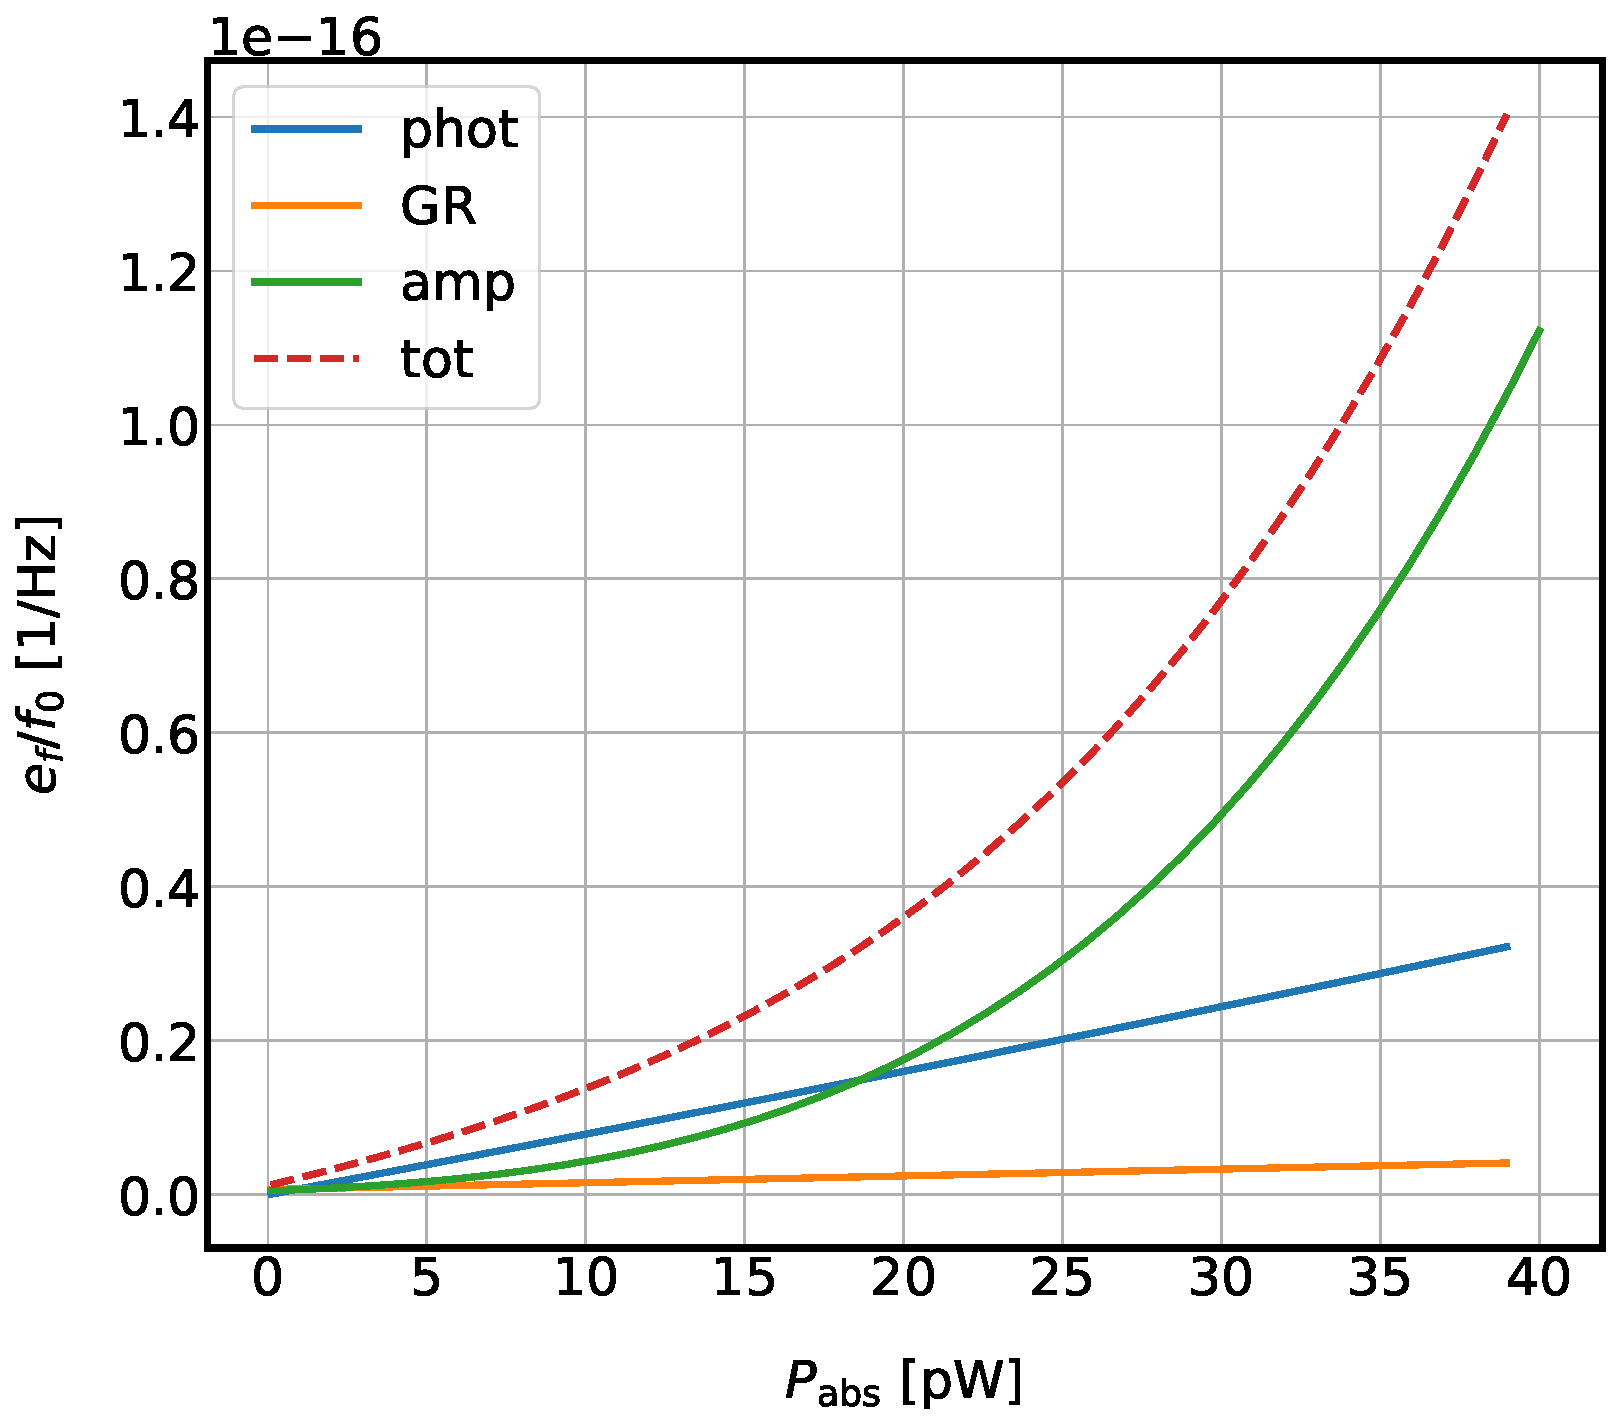
\includegraphics[width=\textwidth]{figures/kid_model/Sxx_fracfreq}
\caption[~The spectral density, in fractional frequency units, as a function of optical power, for the major contributors of instrumental noise.]{The spectral density, in fractional frequency units, as a function of optical power, for the major contributors of instrumental noise.}
\label{fig:Sxx_fracfreq}
\end{figure}

\begin{figure}[!htbp]
\centering
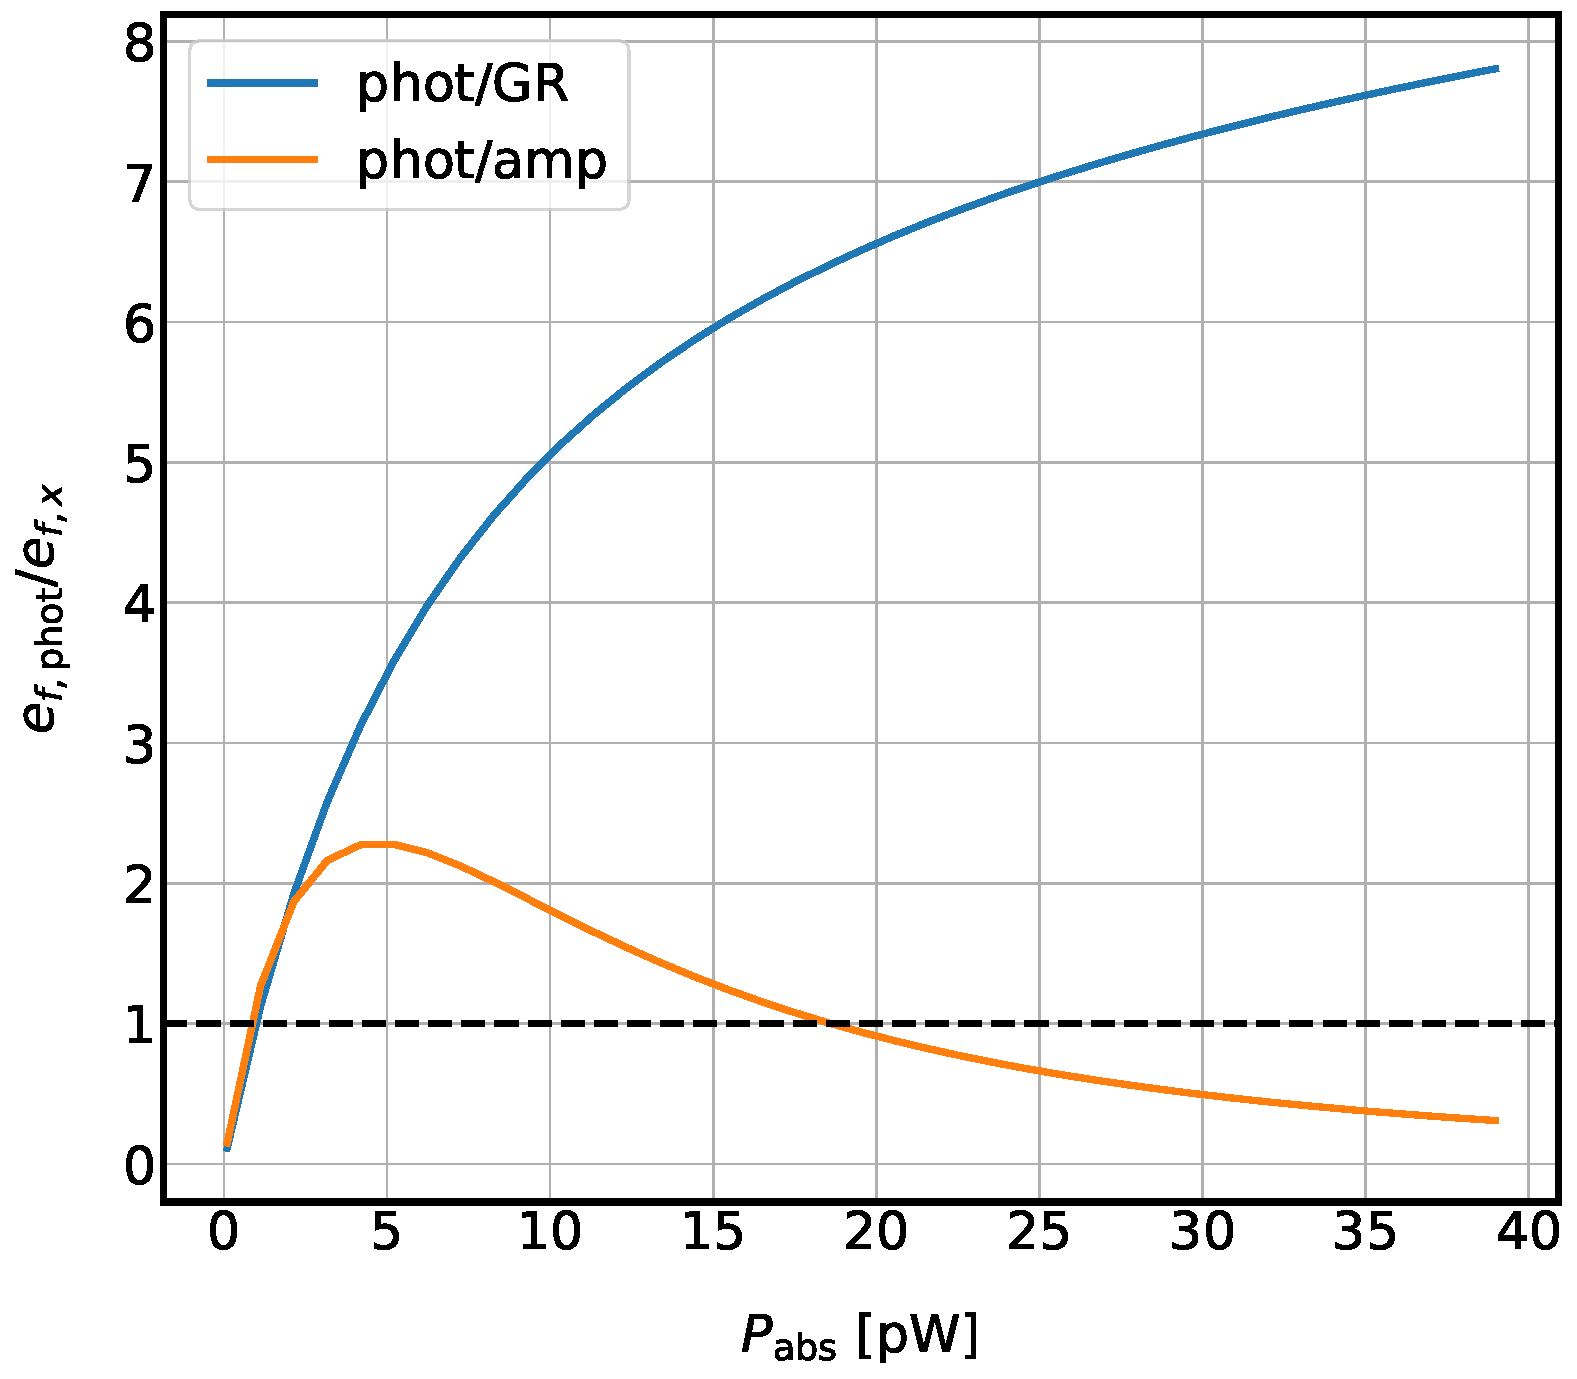
\includegraphics[width=\textwidth]{figures/kid_model/noise_ratios}
\caption[~The simulated ratios of photon to GR and photon to amplifier noise.]{The ratio of $e_{f,phot}$ to $e_{f,GR}$ and $e_{f,\mathrm{amp}}$.}
\label{fig:noise_ratios}
\end{figure}

The total optical NEP is:

\begin{equation} \label{eq:NEP tot}
  NEP_{\mathrm{tot}} = \left( NEP_{\mathrm{amp}}^{2} + NEP_{GR}^{2} + NEP_{TLS}^{2} + NEP_{\mathrm{phot}}^{2} \right)^{1/2} \qquad \left[ \frac{\mathrm{W}}{\sqrt{\mathrm{Hz}}} \right]
\end{equation}

The NEP for each noise source (except for TLS) is shown in Figure~\ref{fig:NEP_tot}. At absorbed powers above a few picowatts, the simulated NEP is $\propto \sqrt{\gls{Popt}}$.

\begin{figure}[!htbp]
\centering
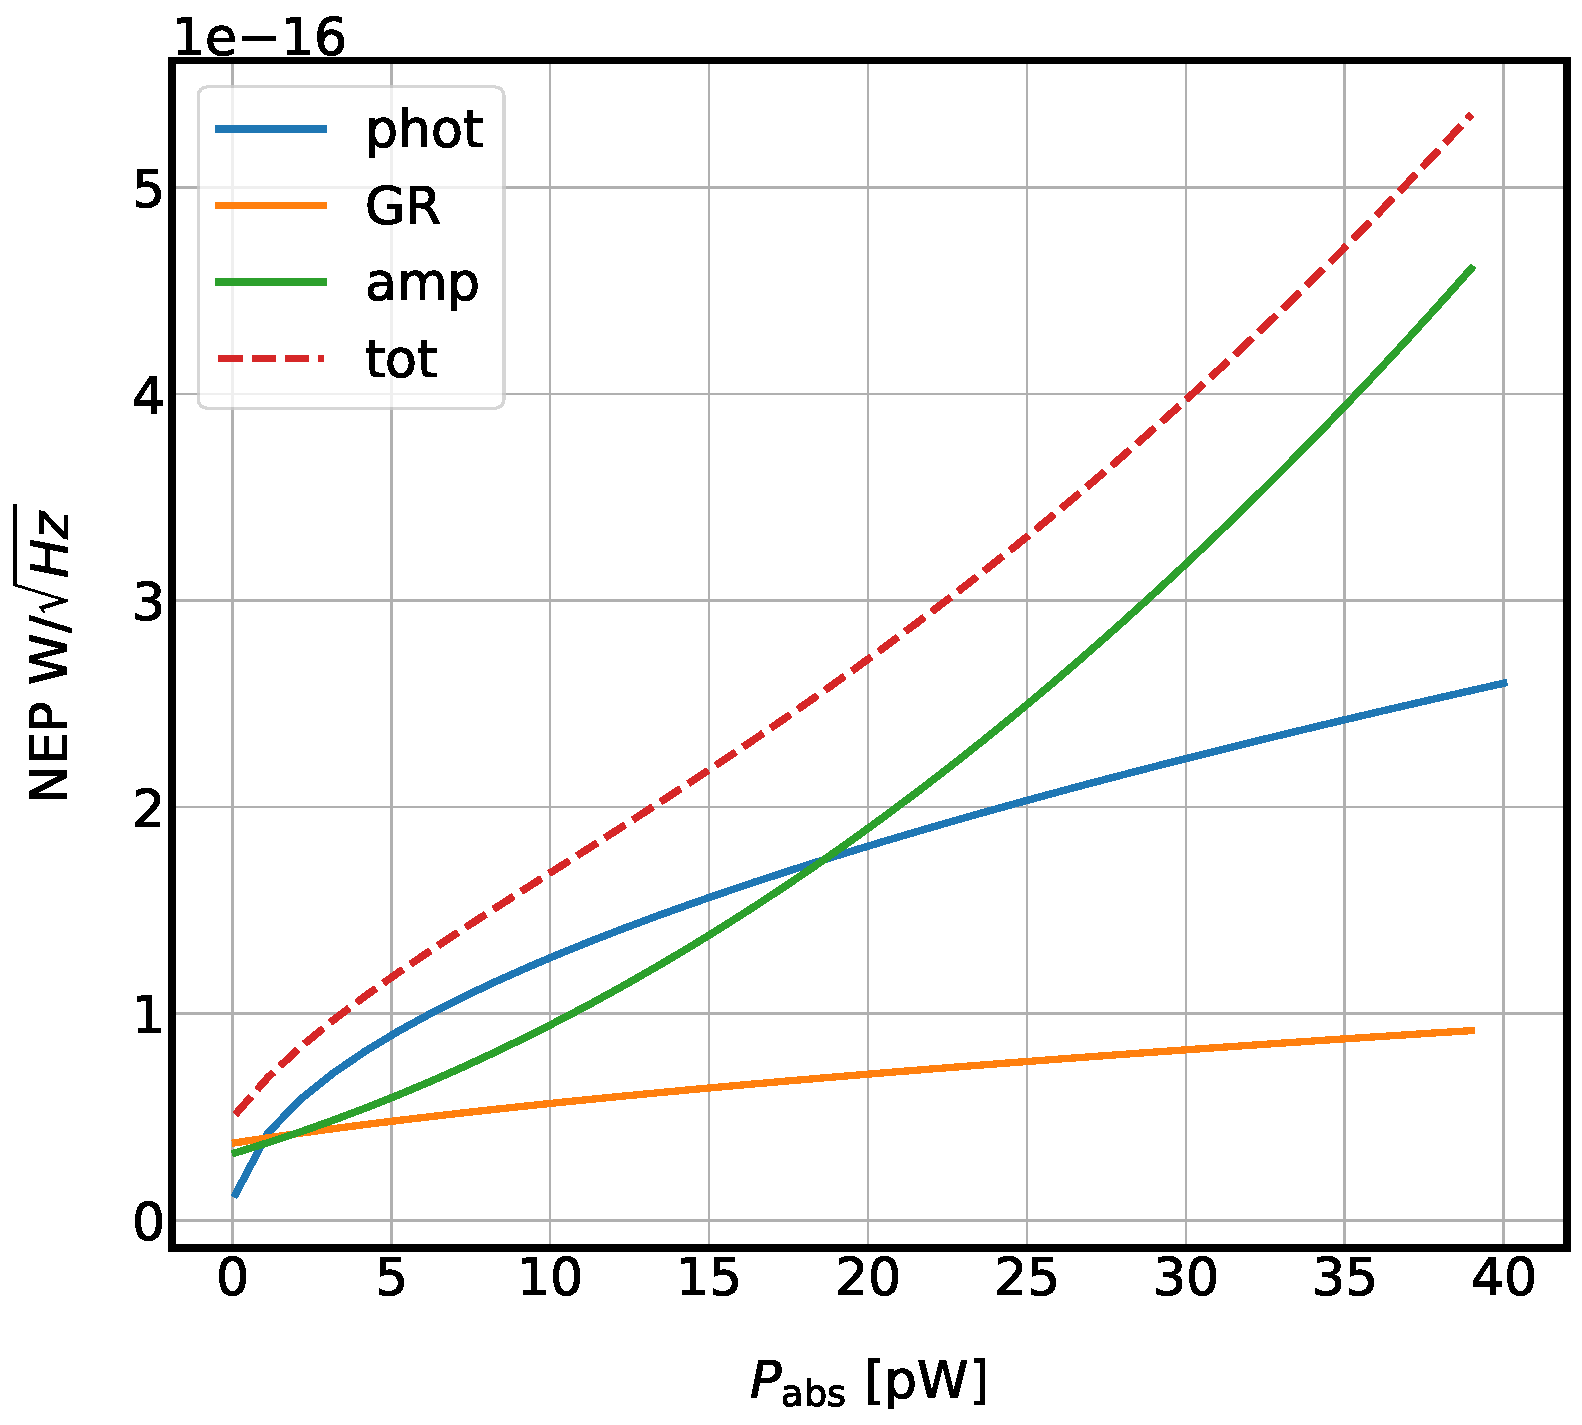
\includegraphics[width=\textwidth]{figures/kid_model/NEP}
\caption[~The optical NEP as a function of optical power, for the major contributors of instrumental noise.]{The optical NEP as a function of optical power, for the major contributors of instrumental noise.}
\label{fig:NEP_tot}
\end{figure}

and the total NET can be calculated as:

\begin{equation} \label{eq:NET tot}
  NET_{\mathrm{tot}} = \frac{NEP_{\mathrm{tot}}}{k\gls{opt_eff}\Delta\nu} \qquad \left[ \frac{\mathrm{K}}{\sqrt{\mathrm{Hz}}} \right]
\end{equation}


\begin{comment}
\begin{equation}
  I = \Re(\gls{S21}) = 1 - \frac{\gls{Qr}}{\gls{Qc}}\frac{1}{1 + 4\gls{Qr}^{2}x^{2}}
\end{equation}

\begin{equation}
  Q = \Im(\gls{S21}) = \frac{\gls{Qr}}{\gls{Qc}} \frac{2\gls{Qr}x}{1 + 4\gls{Qr}^{2}x^{2}}
\end{equation}

\section{Detector Biasing} \label{biasing}
% nonlinearity parameter
\begin{equation}
  \alpha = \frac{2\gls{Qr}^{2}}{\gls{Qc}}\frac{P_{r}}{\omega_{\mathrm{shift}}E_{\star}(x)}
\end{equation}

% y, generator detuning (number of linewidths relative to power shifted, or low-power resonance)
\begin{equation}
  y = \gls{Qr}x = \left(\omega_{probe} - \omega_{shift}\right)/\Delta\omega
\end{equation}
where $\Delta \omega$ is the full-width-half-max (FWHM) width of the resonance.
\end{comment}
